%%
%% memoria.tex
%%
\documentclass[a4paper,12pt]{scrbook}
\pagestyle{headings}

% Paquete para dibujos
\usepackage{tikz}

% Referencias externas
\usepackage{xr-hyper}

% Paquete para generar enlaces clickables
\usepackage[pdftex, breaklinks=false, colorlinks=true, linkcolor=black, anchorcolor=black, urlcolor=blue, citecolor=red]{hyperref}

% Encoding y tratamiento de fuentes
\usepackage[T1]{fontenc}
\usepackage[spanish]{babel}
\usepackage[utf8]{inputenc}

% Paquete con el entorno tabularx, que define un tipo de celda X que hace word-wrapping
\usepackage{tabularx}

\usepackage{float}

% Paquete que provee el comando \FloatBarrier para poner una barrera para floats
\usepackage{placeins}

% Paquete para controlar el interlineado a nivel de entorno
\usepackage{setspace}

% Paquete para la fuente charter
\usepackage{charter}

% Paquete para la fuente helvética
\usepackage[scaled=0.92]{helvet}

% Paquete para GNUPlot
\usepackage{gnuplottex}

% Guiones de hyphenado
\usepackage{hyphenat}

% Extra ToC listings
\usepackage{tocbibind}

% Gráficos
\usepackage{graphicx}

% Para poner figuras una al lado de otra
\usepackage[lofdepth,lotdepth]{subfig}

% Paquete para figuras giradas
\usepackage{rotating}

%%%%%%%%%%%%%%%%%%%%%%%%%%%%%%%%%%%%%%%%%%%%%%%%%%%%%%%%%%%%%%%%%%%%%%%%%%%%%%%%%%%%%%%%%%%%%%%%%%%%%%%%%%%%%%
% Paquetes en local (directorio 'paquetes')

% Fuente para códigos
\usepackage{paquetes/inconsolata}

% Automatiza el resaltado de sintaxis usando pygments
\usepackage{paquetes/minted}

% Soporte de acrónimos
\usepackage[printonlyused]{paquetes/acronym-custom}

% Cambia el nombre del apéndice de bibliografía
\addto\captionsspanish{
\renewcommand\bibname{Bibliografía y referencias}
}

%%%%%%%%%%%%%%%%%%%%%%%%%%%%%%%%%%%%%%%%%%%%%%%%%%%%%%%%%%%%%%%%%%%%%%%%%%%%%%%%%%%%%%%%%%%%%%%%%%%%%%%%%%%%%%

\begin{document}

% Órdenes LaTeX variadas
% http://www.tex.ac.uk/cgi-bin/texfaq2html?label=chngmargonfly

\newenvironment{changemargin}[2]{%
  \begin{list}{}{%
    \setlength{\topsep}{0pt}%
    \setlength{\leftmargin}{#1}%
    \setlength{\rightmargin}{#2}%
    \setlength{\listparindent}{\parindent}%
    \setlength{\itemindent}{\parindent}%
    \setlength{\parsep}{\parskip}%
  }%
  \item[]}{\end{list}}

\newenvironment{nota}{
  \begin{changemargin}{2em}{2em}
    \textbf{\textsc{Nota: }}
}{
  \end{changemargin}
}

\newcommand{\nombreProyecto}{SiteUp: plataforma para la vigilancia de la disponibilidad de servicios de internet}
\newcommand{\jugador}{\textit{Jugador}}
\newcommand{\sistema}{\textit{Sistema}}


% %% PRODUCTOS
% \newcommand{\nombrepostprocesador}{ACL2:\colonhyp{}Procesador}
% \newcommand{\nombrevisor}{XMLEye}
% \newcommand{\nombreyaxml}{YAXML:\colonhyp{}Reverse}
% \newcommand{\postprocesador}{\texttt{\nombrepostprocesador}\xspace}
% \newcommand{\visor}{\nombrevisor\xspace}
% \newcommand{\yaxml}{\texttt{\nombreyaxml}\xspace}

% \newcommand{\biblioteca}[1]{\index{#1}\texttt{#1}}

% % YAML/YAXML
% \newcommand{\etiqueta}[1]{{\bfseries \ttfamily #1}}

% % ACL2

% \newcommand{\orden}[1]{\texttt{#1}}   % Nombre de orden ACL2
% \newcommand{\fichero}[1]{\texttt{#1}} % Nombre de fichero
% \newcommand{\evento}[1]{\texttt{#1}}  % Nombre de un evento
% \newcommand{\libro}[1]{\textsc{#1}}   % Libro ACL2

% % PERL

% \newcommand{\modulo}[1]{\index{módulo Perl!#1}\index{#1|see{módulo Perl!#1}}\texttt{#1}}
% \newcommand{\funcion}[1]{\textit{#1}}

% % JAVA

% \newcommand{\clase}[1]{\textit{#1}}   % Clase Java
% \newcommand{\metodo}[1]{\texttt{#1}}  % Método (también Perl)
% \newcommand{\paquete}[1]{\texttt{#1}}

% %% MANUALES

% \newcommand{\accesoteclado}[1]{\textsc{#1}} % Acceso de teclado

% %% OTROS

% \newcommand{\patron}[1]{\emph{#1}}

% \newcolumntype{,}{>{$}r<{$}}
% \newcommand{\Index}[1]{#1\emph{\index{#1}}}

% \newcounter{pasoacept}

% \newenvironment{pruebaaceptacion}{
%   \setcounter{pasoacept}{0}
%   \begin{center}
%   \begin{tabular}{| >{\stepcounter{pasoacept}\arabic{pasoacept}. }p{.4\linewidth} | p{.5\linewidth}|}
%     \hline
%     \multicolumn{1}{| c |}{\textbf{Paso seguido}} & \multicolumn{1}{c|}{\textbf{Resultado esperado}} \\
%     \hline
%     \hline
% }{
%   \hline
%   \end{tabular}
%   \end{center}
% }

% \renewcommand{\lstlistlistingname}{Listados}
% \renewcommand{\lstlistingname}{Listado}

% \newcommand{\CPP}
% {\mbox{C\hspace{-.1em}\raise.2ex\hbox{+\hspace{-.1em}+}}\xspace}

% \setlength{\extrarowheight}{4pt}

% \lstset{
%   extendedchars,
%   flexiblecolumns,
%   stringstyle=\ttfamily,
%   showstringspaces=false,
%   frame=tb
% }

% %% PARTE DE DOCBOOK

% \newcommand{\application}[1]{\index{#1}\emph{#1}}
% \newcommand{\cmdsynopsis}[1]{\nohyphens{\texttt{#1}}}
% \newcommand*{\command}[1]{\nohyphens{\textbf{\texttt{#1}}}}
% \newcommand{\constant}[1]{\texttt{#1}}
% \newcommand{\computeroutput}[1]{#1}
% \newcommand*{\email}[1]{\nohyphens{\texttt{#1}}}
% \newcommand*{\envar}[1]{\nohyphens{\texttt{#1}}}
% \newcommand*{\filename}[1]{\texttt{#1}}
% \newcommand*{\guibutton}[2][]{\emph{#2}}
% \newcommand*{\guilabel}[2][]{\emph{#2}}
% \newcommand*{\guimenuitem}[2][]{\emph{#2}}
% \newcommand*{\guimenu}[2][]{\emph{#2}}
% \newcommand*{\keycombo}[1]{\textsc{#1}}
% \newcommand*{\keysym}[1]{\textsc{#1}}
% \newcommand*{\option}[1]{\nohyphens{\texttt{#1}}}
% \newcommand{\prompt}[1]{#1}
% \newcommand{\varname}[1]{\nohyphens{\texttt{#1}}}

% \newcommand{\note}[1]{\vskip 1em
%     \fbox{\parbox{\textwidth}{\textsc{Nota}
%     \vskip 1em #1}} \vskip 1em}


%%% Local Variables:
%%% mode: latex
%%% TeX-master: "memoria"
%%% End:


% Portada
\begin{titlepage}
  \centering
  
\includegraphics[width=.3\textwidth]{0_misc/logo_uca}

  \bigskip
  \bigskip
  \bigskip

  \begin{changemargin}{2em}{2em}
    \centering

    {\Huge \textsc{\nohyphens{Escuela Superior de Ingeniería}}}

    \bigskip
    \bigskip
    \bigskip

    {\huge \nohyphens{Ingeniería Informática}}

    \bigskip
    \bigskip
    \bigskip
    \bigskip
    \bigskip
    \bigskip

    \begin{doublespace}
      {\LARGE \nohyphens{\nombreProyecto}}
    \end{doublespace}


    \bigskip
    \bigskip
    \bigskip
    \bigskip

    \bigskip
    \bigskip
    \bigskip
    \bigskip
    \bigskip
    \bigskip
    \bigskip

  \end{changemargin}

  {\Large José Tomás Tocino García \\}

  \bigskip

  {\large Cádiz, \today}

\end{titlepage}


%%% Local Variables: 
%%% mode: latex
%%% TeX-master: "../memoria"
%%% End: 

\cleardoublepage

% Segunda portada
{
  \thispagestyle{empty}
  \centering
  
\includegraphics[width=.2\textwidth]{0_misc/logo_uca}

  \bigskip
  \bigskip
  \bigskip
  
  \begin{changemargin}{3em}{3em}

    \begin{center}
      {\Huge \textsc{\nohyphens{Escuela Superior de Ingeniería}}}
      
      \bigskip
      \bigskip
      
      {\huge \nohyphens{Ingeniería Técnica en Informática de Sistemas}}
      
      \bigskip
      \bigskip
      \bigskip
      \bigskip
      
      \begin{doublespace}
        {\LARGE \nohyphens{\nombreProyecto}}
      \end{doublespace}


      \bigskip
      \bigskip
      \bigskip
      \bigskip
      
    \end{center}
  \end{changemargin}
  \begin{changemargin}{3em}{1em}
  \begin{flushleft}
    \Large

    \textsc{Departamento}: \nohyphens{Lenguajes y Sistemas Informáticos.} \\
    \textsc{Director del proyecto}: \nohyphens{Antonio García Domínguez y Manuel Palomo Duarte.} \\
    \textsc{Autor del Proyecto}: \nohyphens{José Tomás Tocino García}. \\
  \end{flushleft}

  \end{changemargin}  

  \bigskip
  \bigskip
  \bigskip
  
  \begin{flushright}
    \large
    Cádiz, \today

    \bigskip
    \bigskip
    \bigskip
    \bigskip    
    \bigskip
    \bigskip

    Fdo.: José Tomás Tocino García
    
  \end{flushright}

}

%%% Local Variables: 
%%% mode: latex
%%% TeX-master: "./memoria"
%%% End: 

\cleardoublepage

% Texto de licencia (pequeño)
\bigskip
\bigskip

Este documento se halla bajo la licencia \ac{FDL}. Según estipula la
licencia, se muestra aquí el aviso de copyright. Se ha usado la
versión inglesa de la licencia, al ser la única reconocida
oficialmente por la \ac{FSF}.

\begin{quote}
  Copyright \copyright~\the\year~José Tomás Tocino García.

  Permission is granted to copy, distribute and/or modify this document
  under the terms of the GNU Free Documentation License, Version 1.2
  or any later version published by the Free Software Foundation;
  with no Invariant Sections, no Front-Cover Texts, and no Back-Cover Texts.
  A copy of the license is included in the section entitled "GNU
  Free Documentation License".
\end{quote}

%%% Local Variables: 
%%% mode: latex
%%% TeX-master: "../memoria"
%%% End: 

\cleardoublepage

% Agradecimientos
\section*{Agradecimientos}
Quiero agradecer y dedicar la presente memoria y, por extensión, el proyecto
SiteUp al completo:

\begin{itemize}
\item A mi familia y mi pareja, que igualmente como ocurrió durante el
  desarrollo del PFC de la Ingeniería Técnica allá en 2011, han tenido que
  \textit{soportar} el desarrollo de este PFC durante bastante tiempo.

\item A Manuel Palomo, Rafael R. Galván, Juan M. Dodero e Iván Ruiz. Gracias a
  ellos he formado parte de la UCA como becario, como alumno colaborador y como
  personal investigador desde 2009 hasta 2013, un periodo en el que he aprendido
  más de lo imaginable.
 
\item A mis compañeros más cercanos de la carrera, que me han apoyado y de los
  que me he nutrido para desarrollar este proyecto.

\item A Guido Van Rossum por crear Python, un lenguaje precioso que hace fácil
  hasta las tareas más complejas y pone de manifiesto las obvias limitaciones de
  otros lenguajes más populares como PHP. Sin Python, este proyecto no sería nada.
\item A los creadores de Django, por desarrollar una pieza de software tan
  lógica y a la vez tan potente y útil. 

\item A los que apuestan por el software libre y el conocimiento abierto. Sus
  herramientas, bibliotecas y documentos han hecho posible que SiteUp llegase a
  buen puerto.
\end{itemize}


\cleardoublepage

% Índices varios
\tableofcontents
\listoffigures
%\listoftables

\setlength{\parskip}{1.2ex plus 0.4ex minus 0.1ex}

\chapter{Introducción}
\label{chap:introduccion}
\section{Contexto y motivación}
Las tecnologías de la información en general e Internet en particular son ya
parte integral de la sociedad. Casi todos los ámbitos de la vida diaria de las
personas, desde las interacciones sociales hasta la búsqueda de empleo, cuentan
ya con su reflejo en las tecnologías de la información, a menudo mediante el uso
de servicios web a través de Internet. 

No solo los aspectos tradicionales de la sociedad tienen su presencia en las
redes, también han surgido nuevos modelos empresariales propios de Internet que
han crecido de manera importante y se han situado a niveles comparables a los de
las empresas tradicionales. Empresas puramente digitales como Facebook o Twitter
ya cotizan en bolsa y realizan operaciones bursátiles del orden de miles de
millones de dólares.

Se pone pues de manifiesto la importancia de la fiablidad de los servicios e
infraestructuras de los que dependen estos nuevos modelos de negocio. El
\textit{uptime} -- un término inglés que describe el porcentaje de tiempo que un
servicio se mantiene disponible -- debe ser siempre cercano al 100\%, dado que
en caso contrario los potenciales usuarios del servicio se encontrarán con que
no pueden acceder a él, dando lugar incluso a pérdidas económicas. Es el caso de
Amazon, que llegó a perder 4.8 millones de dólares al sufrir un fallo que dejó
inaccesible su web durante 40 minutos~\cite{amazon}.

De todo lo expuesto se extrae la necesidad de contar con sistemas para
monitorizar la disponibilidad de estos servicios y, en caso necesario, actuar de
manera que puedan subsanarse las causas de los problemas.

\section{Objetivos}
\label{sec:objetivos}

A la hora de definir los objetivos de un sistema, podemos agruparlos
en dos tipos diferentes: \textbf{funcionales} y
\textbf{transversales}. Los primeros se refieren a \textit{qué} debe
hacer la aplicación que vamos a desarrollar, e inciden
directamente en la experiencia del usuario y de potenciales
desarrolladores.

Por otro lado, los objetivos transversales son aquellos invisibles al
usuario final, pero que de forma inherente actúan sobre el resultado
final de la aplicación y sobre la experiencia de desarrollo de la misma.

\subsection{Funcionales}
\begin{itemize}
\item Crear un conjunto de herramientas para la monitorización y el chequeo de
  diversos aspectos del estado de un servicio de Internet.
\item Crear una aplicación online, de acceso público, que permita la creación y
  gestión de chequeos de manera sencilla, basada internamente en las
  herramientas mencionadas en el punto anterior.
\item Habilitar esta aplicación de un sistema de notificaciones mediante correo
  electrónico que alerte a los usuarios de posibles cambios en la disponibilidad
  de los servicios monitorizados.
\item Crear una aplicación móvil para el sistema operativo Android para la
  recepción instantánea de avisos provenientes de la aplicación web.
\end{itemize}

\subsection{Transversales}
\begin{itemize}
\item Investigar y conocer los vectores de vigilancia usados habitualmente para
  monitorizar servicios de Internet.
\item Ampliar mis conocimientos sobre desarrollo web en general y las
  tecnologías de back-end en particular.
\item Adquirir soltura en el uso del lenguaje de programación Python en entornos
  web.
\item Obtener una base de conocimientos mínima sobre el desarrollo de
  aplicaciones sobre la plataforma móvil Android.
\item Utilizar un enfoque de análisis, diseño y codificación orientado
  a objetos, de una forma lo más clara y modular posible, para
  permitir ampliaciones y modificaciones sobre la aplicación por
  terceras personas.
\item Hacer uso de herramientas básicas en el desarrollo de software,
  como son los \textbf{Sistemas de Control de Versiones} para llevar
  un control realista del desarrollo del software, así como hacer de
  las veces de sistema de copias de seguridad.
\end{itemize}


\section{Alcance}
\textbf{SiteUp} se modela como una herramienta de monitorización de servicios de
internet accesible a través de la web. Los usuarios tendrán la posibilidad de
crear y gestionar una serie de \textit{chequeos} de diversos tipos sobre los
servicios web que elijan. La aplicación irá recopilando información relativa a
esos chequeos, e informará al usuario en caso de que las verificaciones que se
hayan dado de alta no coincidan con los resultados obtenidos.

Además, el usuario tendrá la posibilidad de recibir notificaciones de manera
instantánea a través del correo electrónico y de una aplicación para la
plataforma móvil Android. El servicio web estará totalmente adaptado para su uso
en dispositivos móviles.

\subsection{Limitaciones del proyecto}
Aunque cubre una gran parte de los puntos de vigilancia habituales, la
aplicación se limita a ofrecer chequeo de respuesta de ping, chequeo de puertos,
chequeo de registros DNS y chequeo de cabeceras y contenidos HTTP. 

La aplicación de Android no cuenta con ninguna funcionalidad para gestionar los
chequeos de un usuario, sino que sirve para recibir notificaciones instantáneas
provenientes de la aplicación web. Ésta, por otro lado, está completamente
adaptada para su uso a través de dispositivos móviles gracias al uso del
\textit{responsive web design}.

Idealmente los chequeos deberían hacerse simultáneamente desde diferentes
máquinas colocadas en diversos puntos geográficos, para así tener unos
resultados más fiables. La falta de infraestructuras y la finalidad didáctica
del proyecto han limitado la aplicación a una estructura monolítica en la que
los chequeos se hacen desde una sola máquina, la misma que sirve el servicio
web.

\subsection{Licencia}
El proyecto está publicado como software libre bajo la licencia
\ac{GPL} versión 3. El conjunto de bibliotecas y módulos utilizados
tienen las siguientes licencias:

\begin{itemize}

\item El framework de desarrollo web en el que se basa la aplicación es
  \textbf{Django}~\cite{django}, que utiliza la licencia
  \textit{\ac{BSD}}~\footnote{\url{https://github.com/django/django/blob/master/LICENSE}}.

\item El servidor web \textbf{nginx}~\cite{nginx} también utiliza la licencia \textit{BSD}.

\item Los siguientes paquetes de Python utilizan también la licencia \textit{BSD}:
  \begin{itemize}
  \item Celery
  \item Sqlparse
  \item iPython
  \item dnspython
  \item coverage
  \item django-rest-framework
  \item billiard
  \item anyjson
  \item Fabric
  \end{itemize}

\item Los siguientes paquetes de Python utilizan la licencia \textit{\ac{MIT}}:
  \begin{itemize}
  \item PyDot
  \item Gunicorn
  \item Requests
  \item django-extensions
  \item six
  \item sh
  \item pip
  \item virtualenvwrapper
  \item factory-boy
  \end{itemize}

\end{itemize}

\section{Estructura del documento}
El presente documento se rige según la siguiente estructura:

\begin{itemize}
\item \textbf{\nameref{chap:introduccion}}. Se exponen las motivaciones y
  objetivos detrás del proyecto \textbf{SiteUp}, así como información sobre las
  licencias de sus componentes, glosario y estructura del documento.
\item \textbf{\nameref{chap:calendario}}, donde se explica la planificación del
  proyecto, la división de sus etapas, la extensión de las etapas a lo largo del
  tiempo y los porcentajes de esfuerzo.
\item \textbf{\nameref{chap:fundamentos}}, que explica las labores de
  documentación y experimentación previas al desarrollo, que han servido para
  labrar una base de conocimientos que nos diera las suficientes garantías para
  afrontar el proyecto.
\item \textbf{\nameref{chap:analisis}}. Se detalla la fase de análisis del
  sistema, explicando los requisitos funcionales del sistema, los diferentes
  casos de uso, así como las principales operaciones con sus diagramas de
  secuencia y contratos.
\item \textbf{\nameref{chap:diseno}}. Seguido del análisis, se expone en detalle
  la etapa de diseño del sistema, con los diagramas de clases.
\item \textbf{\nameref{chap:implementacion}}. Una vez analizado el sistema y
  definido su diseño, en esta parte se detallan las decisiones de implementación
  más relevantes que tuvieron lugar durante el desarrollo del proyecto.
\item \textbf{\nameref{chap:pruebas}}. Listamos y describimos las pruebas que se
  han llevado a cabo sobre el proyecto para garantizar su fiabilidad y
  consistencia.
\item \textbf{\nameref{chap:conclusiones}}. Comentamos las conclusiones a las
  que se han llegado durante el transcurso y al término del proyecto.
\end{itemize}

Y los siguientes apéndices:
\begin{itemize}
\item \textbf{\nameref{chap:herramientas}}, donde detallamos qué hemos usado para la
  elaboración del proyecto.
\item \textbf{\nameref{chap:manual_instalacion}} del proyecto en sistemas nuevos.
\item \textbf{\nameref{chap:manual_usuario}}, donde se explica cómo usar la aplicación.
\end{itemize}

\subsection{Acrónimos}

\begin{acronym}
  \acro{IANA}{Internet Assigned Numbers Authority}
  \acro{IETF}{Internet Engineering Task Force}
  \acro{Sass}{Syntactically Awesome Style Sheets}
  \acro{AJAX}{Asynchronous JavaScript and XML}
  \acro{SQL}{Structured Query Language}
  \acro{ORM}{Object-relational mapping}
  \acro{AMQP}{Advanced Message Queuing Protocol}
  \acro{LOPD}{Ley Orgánica de Protección de Datos}
  \acro{WSGI}{Web Server Gateway Interface}
  \acro{PSFL}{Python Software Foundation License}
  \acro{ABI}{Application Binary Interface}
  \acro{ACL2s}{ACL2 Sedan}
  \acro{ACL2}{A Computational Logic for Applicative Common Lisp}
  \acro{ALSA}{Advanced Linux Sound Architecture}
  \acro{AMD}{Advanced Micro Devices}
  \acro{API}{Application Programming Interface}
  \acro{APL}{Apache Public License}
  \acro{ASCII}{American Standard Code for Information Interchange}
  \acro{BNF}{Backus-Naur Form}
  \acro{BOM}{Byte Order Mark}
  \acro{BSD}{Berkeley Software Distribution}
  \acro{C3}{Chrysler Comprehensive Compensation System}
  \acro{CAP}{Complex Arithmetic Processor}
  \acro{CASE}{Computer Assisted Software Engineering}
  \acro{CRUD}{Create-Read-Update-Delete}
  \acro{CD}{Compact Disc}
  \acro{CPAN}{Comprehensive Perl Archive Network}
  \acro{CPU}{Central Processing Unit}
  \acro{CSS}{Cascading Style Sheet(s)}
  \acro{CVS}{Concurrent Versions System}
  \acro{DDR}{Dance Dance Revolution}
  \acro{DNS}{Domain Name Server}
  \acro{DOM}{Document Object Model}
  \acro{DFT}{Discrete Fourier Transform}
  \acro{DSP}{Digital Signal Processing}
  \acro{DTD}{Do\-cu\-ment Type De\-fi\-ni\-tion}
  \acro{EAFP}{Easier to Ask for Forgiveness than Permission}
  \acro{FDL}{Free Documentation License}
  \acro{FFT}{Fast Fourier Transform}
  \acro{FSF}{Free Software Foundation}
  \acro{GCC}{GNU Compiler Collection}
  \acro{GCJ}{GNU Compiler for Java}
  \acro{GCL}{GNU Common Lisp}
  \acro{GIMP}{\acs{GNU} Image Manipulation Program}
  \acro{GML}{Generalized Markup Language}
  \acro{GNU}{GNU is Not Unix}
  \acro{GPL}{General Public License}
  \acro{GTK+}{\acs{GIMP} Toolkit}
  \acro{GUI}{Graphical User Interface}
  \acro{HTML}{Hyper Text Markup Language}
  \acro{HTTP}{Hyper Text Transfer Protocol}
  \acro{IBM}{International Business Machines}
  \acro{ICMP}{Internet Control Message Protocol}
  \acro{IDE}{Integrated Development Environment}
  \acro{IEEE}{Institute of Electrical and Electronics Engineers}
  \acro{IIS}{Internet Information Server}
  \acro{ISP}{Internet Service Provider}
  \acro{IP}{Internet Protocol}
  \acro{J2SE}{Java 2 Standard Edition}
  \acro{JACK}{JACK Audio Connection Kit}
  \acro{JAXP}{Java API for XML Parsing}
  \acro{JDBC}{Java DataBase Connectivity}
  \acro{JDK}{Java Development Kit}
  \acro{JIT}{Just In Time}
  \acro{JRE}{Java Runtime Environment}
  \acro{JSON}{JavaScript Object Notation}
  \acro{JSR}{Java Specification Request}
  \acro{JVM}{Java Virtual Machine}
  \acro{LGPL}{Lesser General Public License}
  \acro{LTS}{Long Time Support}
  \acro{MDI}{Multiple Document Interface}
  \acro{MIDI}{Musical Instrument Digital Interface}
  \acro{MIT}{Massachusetts Institute of Technology}
  \acro{MP3}{MPEG-2 Audio Layer III}
  \acro{MVC}{Model View Controller}
  \acro{MVP}{Model View Presenter}
  \acro{ODF}{Open Document Format}
  \acro{OSS}{Open Sound System}
  \acro{PAR}{Perl ARchive Toolkit}
  \acro{PCM}{Pulse-Code Modulation}
  \acro{PDF}{Portable Document Format}
  \acro{POD}{Plain Old Do\-cu\-men\-ta\-tion}
  \acro{POSIX}{Portable Operating System Interface, UniX based}
  \acro{Perl}{Practical Extraction and Report Language}
  \acro{RPM}{RPM Package Manager}
  \acro{RUP}{Rational Unified Process}
  \acro{RTP}{Real-time Transport Protocol}
  \acro{SAX}{Simple API for XML}
  \acro{SDI}{Single Document Interface}
  \acro{SDL}{Simple DirectMedia Layer}
  \acro{SGML}{Standard Generalized Markup Language}
  \acro{SSL}{Secure Sockets Layer}
  \acro{SVG}{Structured Vector Graphics}
  \acro{SWT}{Standard Widget Toolkit}
  \acro{TCK}{Technology Compatibility Kit}
  \acro{TDI}{Tabbed Document Interface}
  \acro{UML}{Unified Modelling Language}
  \acro{URI}{Uniform Resource Identifier}
  \acro{URL}{Uniform Resource Locator}
  \acro{UTF}{Universal Transformation Format}
  \acro{VPS}{Virtual Private Server}
  \acro{W3C}{World Wide Web Consortium}
  \acro{WWW}{World Wide Web}
  \acro{XHTML}{eXtensible Hyper Text Markup Language}
  \acro{XML}{eXtensible Markup Language}
  \acro{XP}{eXtreme Programming}
  \acro{XSL-FO}{eXtensible Stylesheet Language Formatting Objects}
  \acro{XSLT}{eXtensible Stylesheet Language Transformations}
  \acro{XSL}{eXtensible Stylesheet Language}
  \acro{YAML}{YAML Ain't a Markup Language}
  \acro{YAXML}{YAML XML binding}
\end{acronym}



%%% Local Variables:
%%% mode: latex
%%% TeX-master: "../memoria"
%%% End:


\chapter{Planificación}
\label{chap:calendario}
El proyecto no se ha desarrollado siguiendo un calendario estricto,
dado que era imposible cuantificar el tiempo que tomaría el adquirir
las bases teóricas necesarias para poder afrontarlo con garantías. Su
desarrollo se ha compaginado con los estudios del último curso de
Ingeniería Técnica en Informática de Sistemas y las labores como
becario en la Oficina de Software Libre y Conocimiento Abierto de la
Universidad de Cádiz~\cite{osluca}.

\section{Iteraciones}
Para la realización del proyecto se ha utilizado un modelo de desarrollo
iterativo incremental. En la redacción del presente documento se presentarán la
fase de investigación preliminar y las etapas de análisis, diseño,
implementación y pruebas del proyecto en su estado final. A continuación se
detallan cada una de las iteraciones por las que ha ido pasando el proyecto.

\subsection{Primera iteración: conocimientos preliminares}
Antes de poder comenzar con el análisis y diseño del propio proyecto,
era esencial adquirir una serie de conocimientos para poder afrontar
su desarrollo con todas las garantías. Durante esta iteración, se
llevaron a cabo labores de documentación y aprendizaje autodidacta con
las que se asentaron los conocimientos necesarios.

Además, durante este periodo también se barajaron las diferentes
posibilidades de implementación del sistema, así como las posibles
herramientas y bibliotecas de terceros que pudieran ser de ayuda.

\subsection{Segunda iteración: analizador básico}
Una vez adquiridos los conocimientos teóricos necesarios, y decididas
las técnicas y herramientas para llevar aquellos a la práctica, fue
obvia la necesidad de empezar por diseñar un analizador de notas
básico, que sería el corazón del programa. Del éxito del desarrollo
temprano del módulo que se encargaría del análisis de sonidos
dependería la viabilidad completa del proyecto.

\subsection{Tercera iteración: interfaz gráfica de usuario}
Con el módulo de análisis desarrollado, \textit{sólo} restaba
desarrollar el resto de la aplicación alrededor del mismo. En esta
tercera iteración se propusieron numerosos diseños para la interfaz
gráfica de usuario y, una vez decantados por uno de ellos, comenzó el
desarrollo de los elementos de la interfaz, haciendo énfasis en
conseguir un aspecto dinámico y jovial.

\subsection{Cuarta iteración: motor de lecciones}
Uno de los subproductos de la aplicación es el motor de lecciones, que
presenta una serie de unidades didácticas en formato multimedia,
compuestas de imágenes y textos, con conceptos sobre música. En esta
iteración se hizo un análisis de las posibilidades de este motor,
concluyendo con el diseño y desarrollo de un mecanismo muy sencillo de
ampliar y utilizar.

\subsection{Quinta iteración: motor de canciones}
La parte de mayor interactividad de la aplicación es el motor de
canciones, en el que el usuario tiene la posibilidad de tocar una
canción que aparece en pantalla, usando la flauta, mientras la
aplicación valora en tiempo real su interpretación. Durante la quinta
iteración se elaboró este sistema, encargado de listar y cargar las
diferentes canciones, y puntuar al usuario según cómo lo haga.

\section{Diagrama de Gantt}
Se ha diseñado un diagrama de Gantt para reflejar la distribución de las tareas
a lo largo del tiempo (figura~\ref{fig:gantt} en la página~\pageref{fig:gantt}).

\begin{figure}
  \centering
  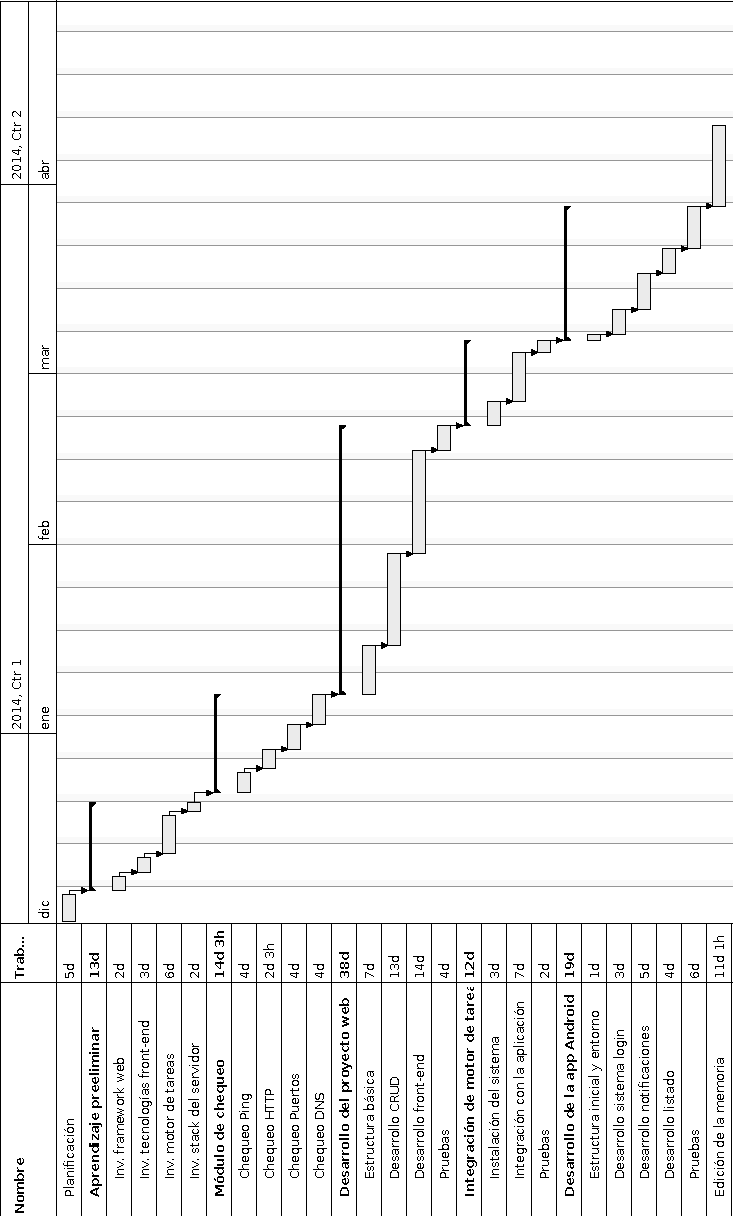
\includegraphics[width=0.95\textwidth]{2_calendario/imagen_diagrama_gantt}
  \caption{Diagrama Gantt de iteraciones}
  \label{fig:gantt}
\end{figure}

%%% Local Variables: 
%%% mode: latex
%%% TeX-master: "../memoria"
%%% End: 


\chapter{Requisitos del sistema}
\label{chap:fundamentos}
En este capítulo se presentan los detalles de diseño del proyecto, basándonos en
el análisis mostrado en los anteriores apartados. Se detallan la arquitectura
general y el diseño físico de datos entre otros aspectos.

\section{Arquitectura del sistema}

\subsection{Arquitectura física}
\label{sec:arquitectura-fisica}

En este apartado, describimos los principales componentes hardware que forman la
arquitectura física de nuestro sistema, recogiendo por un lado los componentes
del servidor de producción y, por otro lado, los componentes del cliente de acceso.

\subsubsection{Servidor de producción}
\label{subsec:entorno-produccion}

\paragraph{Hardware}

El hardware mínimo indispensable para la correcta ejecución del motor del
proyecto se detalla en la siguiente lista:

\begin{itemize}
\item 512MiB de memoria RAM como mínimo.
\item 10GiB de disco duro como mínimo.
\item Acceso a Internet con un canal de subida de al menos 1Mbit/s.
\end{itemize}

\paragraph{Software}

En cuanto al software necesario para la ejecución del proyecto, se detallan los
siguientes elementos, que es necesario instalar para desplegar el sistema:

\begin{itemize}
\item Sistema operativo \textbf{GNU/Linux}, preferiblemente basado en paquetería Debian.
\item Código fuente del proyecto \textbf{SiteUp}.
\item Servidor de shell remota \textbf{SSH}, accesible desde el exterior.
\item \textbf{Nginx}, servidor web trabajando en modo de proxy inverso.
\item \textbf{Supervisord}, sistema para el control de procesos que trabajen en modo demonio..
\item \textbf{RabbitMQ}, cola de tareas sencilla que cumple el estandar \ac{AMQP}.
\item Intérprete de \textbf{Python}, versión mínima 2.7.
\item Soporte de entornos virtuales \textbf{VirtualEnv} para la encapsulación de
  dependencias.
\end{itemize}

% Una vez satisfechos los anteriores requisitos, el proyecto SiteUp instalará una
% serie de dependencias propias, de forma encapsulada dentro de un entorno
% virtual. Algunas de las dependencias más importantes son:

% \begin{itemize}
% \item \textbf{Django}, framework web en el que se basa el proyecto.
% \item \textbf{Celery}, cola de tareas asíncronas.
% \item \textbf{Fabric}, servicio para la creación de scripts de despligue en servidores remotos.
% \item \textbf{Gunicorn}, servidor para aplicaciones web desarrolladas en Python
%   basadas en el estándar WSGI.
% \item Bibliotecas auxiliares para el lanzamiento de diversos tipos de chequeos
%   en red: \textbf{requests}, \textbf{dnspython} y \textbf{urllib}.
% \end{itemize}

% De igual modo para el desarrollo del lado \textit{front-end} de la web existen
% ciertas dependencias, instalables en forma de módulos de Node JS. Las
% dependencias más importantes son:

% \begin{itemize}
% \item \textbf{Sass}, lenguaje de hojas de estilo que amplía las funcionalidades
%   de CSS. El código Sass compila a código CSS válido.
% \item \textbf{Compass}, framework para Sass que añade numerosas funciones y
%   \textit{mixins} para facilitar el desarrollo front-end.
% \item \textbf{Grunt}, un lanzador que automatiza la ejecución de tareas comunes
%   y tediosas escrito en JavaScript.
% \end{itemize}

\subsubsection{Cliente de acceso web}

El requisito no funcional NRQ-4, presente en el cuadro~\ref{tab:accesibilidad}
indica que la plataforma web deberá ser accesible desde cualquier clase de
dispositivo con acceso a Internet. Así pues, la única restricción disponible
para los clientes es que cuenten con un navegador modern que provea de acceso
web y sea compatible con los últimos estándares web.

\subsubsection{Cliente de acceso Android}

Los clientes que quieran acceder mediante la aplicación Android deberán contar
con un dispositivo que soporte como mínimo la versión 2.3 del sistema operativo
Android. Además, estos dispositivos deberán tener acceso a Internet en general,
y a los Google Play Services en particular.

\subsection{Arquitectura lógica}

La arquitectura lógica del sistema está formada por los elementos software
(servicios, aplicaciones, librerías, frameworks, etc.) que componen el software
base, más el software desarrollado para cumplir los requisitos de la
aplicación. En esta sección se muestra la organización de los distintos
elementos software que componen el proyecto así como la comunicación entre
ellos. 

\subsubsection{Plataforma web}
\label{subsec:arquitectura-logica-web}

En la figura~\ref{fig:arquitectura-logica} se puede ver un esquema de cómo se
comunican los diferentes elementos que conforma el sistema web a alto nivel. En
detalle, el flujo que sigue en cada capa es el siguiente.

\begin{figure}[htbp]
  \centering
  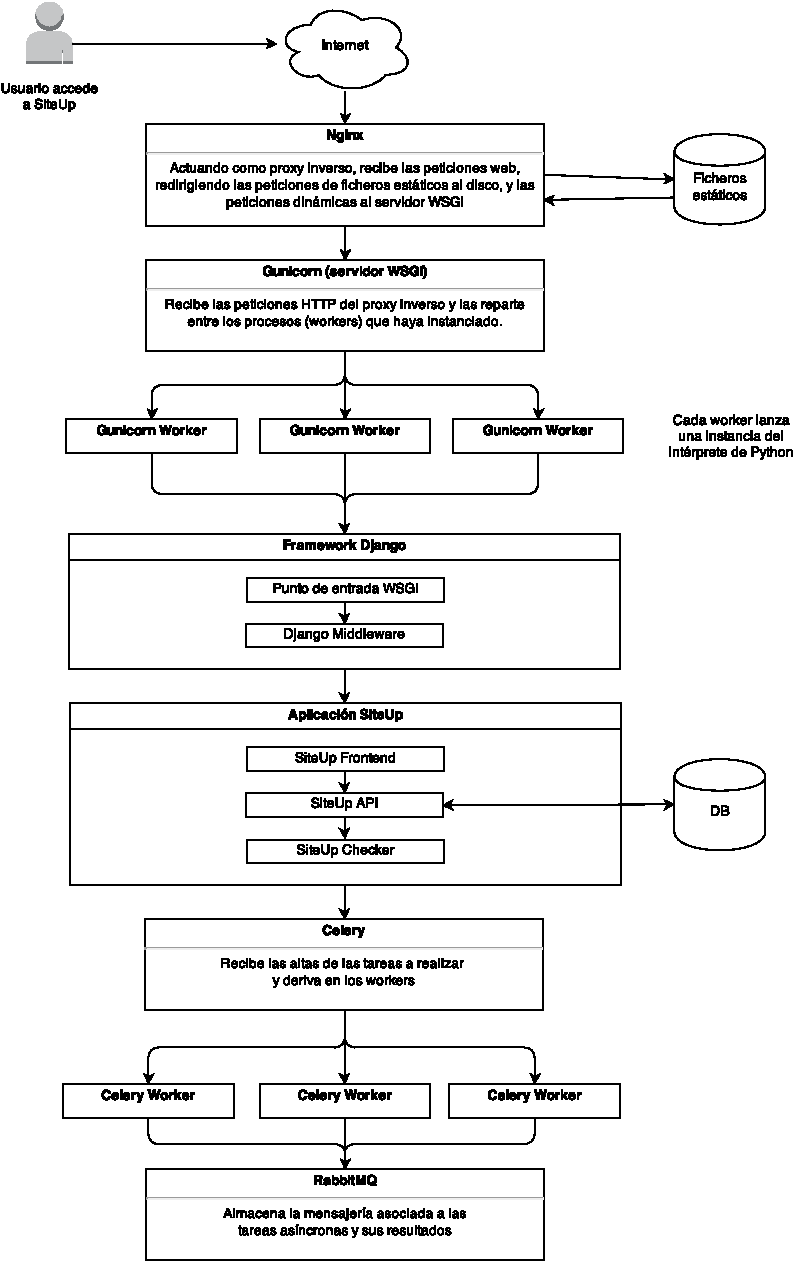
\includegraphics[width=0.9\textwidth]{5_diseno/diagrama_arquitectura_logica}
  \caption{Arquitectura lógica del sistema web}
  \label{fig:arquitectura-logica}
\end{figure}


\paragraph{Navegador}

Cuando un usuario desea acceder a SiteUp, abre un cliente web (habitualmente un
\textbf{navegador} web) y teclea la \ac{URL}. A partir de ahí, el navegador debe
obtener el contenido de la web. Para ello (ignorando cuestiones de bajo nivel,
como el envío de peticiones ARP o resoluciones de DNS) la acción fundamental es
hacer una \textbf{petición HTTP} al servidor que se encuentra en la URL
indicada. Esto se traduce en abrir una conexión TCP al puerto 80 del servidor
remoto y enviar unas cabeceras en las que se indique, entre otras cosas, qué
datos se quiere obtener.

\paragraph{Servidor proxy inverso}

En el servidor debe existir algún \textbf{servicio} que sea capaz de escuchar y
disponer peticiones en el puerto 80 del servidor (el número el puerto puede
variar). En nuestro caso el servidor deberá tener instalado \textbf{Nginx}, un
servidor web/proxy inverso que recibirá las peticiones HTTP del exterior. En
estas peticiones, enviadas por el navegador, se detalla qué recurso se necesita
enviar. 

En el caso de recursos estáticos, como por ejemplo ficheros de imágenes o
archivos de hojas de estilo en cascada (\ac{CSS}), es buena práctica que sea el
propio servidor el que sirva estos ficheros, dado que no necesitan de ningún
procesado dinámico, por lo que no tiene sentido desperdiciar recursos pasando la
petición al código Python.

En el caso de recursos dinámicos, esto es, las peticiones web a páginas
generadas dinámicamente, Nginx actuará de proxy inverso y pasará la petición al
manejador que se haya configurado. 

\paragraph{Servidor de aplicaciones Python}

Como se ha comentado, el proxy inverso ha detectado que hay una petición
dinámica y según su configuración la ha pasado al servidor de aplicaciones
Python. En el caso de nuestro proyecto se tratará del servidor
\textbf{Gunicorn}. Gunicorn sigue un model conocido como \textit{pre-fork
  worker}, que básicamente consiste en instanciar (\textit{forkear}) varios
procesos al lanzar el servidor que se encargarán de procesar las peticiones de
forma paralela, según el proceso padre las vaya repartiendo.

En el mundo del desarrollo web en Python se ha establecido un estándar, conocido
como \ac{WSGI}, que regula la forma en la que las aplicaciones web escritas en
Python se comunican con un servidor web. Por ello, cuando un worker recibe una
petición lo primero que hace es comunicarse con la interfaz WSGI de la
aplicación que se vaya a ejecutar, pasándole la petición y un puntero a un
\textit{callback} al que informar cuando la respuesta a la petición esté
lista. 

\paragraph{Punto de entrada WSGI}

Como se ha comentado, el worker del servidor de aplicaciones se comunica con la
interfaz WSGI. Todas las aplicaciones desarrolladas en Django cuentan con un
módulo \texttt{wsgi.py} que actúa como punto de entrada WSGI y que directamente
pasa la petición al \textit{middleware} de Django que empieza el procesamiento.

\paragraph{Middleware Django y aplicación}

A partir de este punto, la petición va rebotando entre código propio del
framework Django y código de la aplicación. El flujo habitual, en su forma más
básica es el siguiente:

\begin{enumerate}
\item Los módulos de \textit{middleware} que gestionan las peticiones reciben la
  petición actual.
\item Django revisa el fichero \texttt{urls.py} de la aplicación, que contiene
  una lista de URLs asociadas a funciones. Django compara la URL de la petición
  recibida y mira si coincide con alguna de las URLs del proyecto.
\item Si no hay coincidencia, Django devuelve una respuesta negativa,
  normalmente en forma de código de estado 404.
\item Si hay coincidencia, Django llama a la función asociada a esa URL --
  conocida como la \textbf{vista}. La vista procesa la petición, devolviendo una
  respuesta.
\item Esa respuesta hace el camino de forma inversa, pasando por todos los pasos
  hasta el cliente.
\end{enumerate}

Entrando más en detalle, una aplicación de Django se organiza en una
arquitectura de módulos pequeños o \textit{aplicaciones}, cada una de las cuales
debe tener una serire de responsabilidades reducida y acotada, de forma que sea
relativamente sencillo intercambiar las aplicaciones por otras. En el caso del
proyecto SiteUp, se cuenta con tres aplicaciones:

\begin{itemize}
\item \textbf{siteup\_frontend} gestiona las vistas de la aplicación, recibe las
  peticiones, muestra las páginas y gestiona formularios.

\item \textbf{siteup\_api} recibe las órdenes de \texttt{siteup\_frontend},
  haciendo los cambios necesarios en la base de datos, dando de alta las tareas
  y procesando resultados.

\item \textbf{siteup\_checker} cuenta con el código de bajo nivel para hacer los
  chequeos de diferentes tipos. Es principalmente una aplicación tipo
  \textit{helper}.

\end{itemize}

Cada aplicación en Django cuenta con una arquitectura de tres capas conocida
como \textbf{Modelo-Vista-Plantilla}, que se asimila al clásico patrón del
\textbf{Modelo-Vista-Controlador}.

\begin{itemize}
\item El \textbf{modelo} representa la información en la base de datos, evitando
  al usuario tener que utilizar código SQL. Para ello, Django cuenta con un
  \ac{ORM} que facilita el trabajo con registros de la base de datos.
\item Las \textbf{vistas} suelen ser funciones asociadas a una URL. La filosofía
  de Django es que las vistas sirvan solo como \textit{punto de paso} de los
  datos entre los modelos y las plantillas. Es mala práctica colocar lógica de
  negocio compleja en las vistas.
\item Las \textbf{plantillas} son la representación final de los datos, lo que
  acaba viendo el usuario. Las plantillas suelen estar escritas en HTML aunque
  pueden también representarse usando JSON, XML, etc.
\end{itemize}

La organización física de ficheros de un proyecto Django se ajusta perfectamente
a la organización lógica hasta ahora descrita, siendo habitual tener un árbol de
ficheros similar al siguiente:

\begin{itemize}
\item Raíz del proyecto
\item \texttt{siteup} --  Directorio de proyecto general.
  \begin{itemize}
  \item \texttt{settings.py} -- Configuración general.
  \item \texttt{urls.py} -- Configuración de URLs.
  \item \texttt{wsgi.py} -- Punto de acceso WSGI.
  \end{itemize}
\item \texttt{siteup\_api} --  Directorio para la app (suele haber más de uno).
  \begin{itemize}
  \item \texttt{views.py} -- Definición de vistas (funciones).
  \item \texttt{models.py} -- Definición de modelos.
  \item \texttt{tests.py} -- Definición de tests.
  \end{itemize}
\end{itemize}

Opcionalmente, las aplicaciones de Django pueden contar con ficheros
individuales para otros elementos, como formularios, mánagers, migraciones,
validadores, utilidades, filtros, procesadores de contexto, etcétera.

\paragraph{Servidor de tareas asíncronas}

Habrá peticiones en SiteUp cuyo objetivo sea dar de alta chequeos. Éstos dan
lugar a nuevas tareas que serán ejecutadas asíncronamente. Celery, el servidor
de tareas que se utiliza, cuenta con una arquitectura de \textit{workers}
similar a Gunicorn, que se reparten las tareas que son dadas de alta por
SiteUp. Estas tareas se ejecutan de forma periódica. 

Tras su conclusión, Celery se comunica con Django para dejar constancia de los
resultados de esas tareas en forma de modelos de la base de datos.

\paragraph{Broker de mensajes}

Por debajo de Celery se encuentra el \textit{bróker} de mensajes, que implementa
el ya mencionado estándar \ac{AMQP}. El bróker se encarga de almacenar las
tareas y sus resultados en forma de mensajes en una cola. 

En este proceso es necesario \textit{traducir} las tareas a un formato que sea
almacenable y gestionable en una cola. En el caso de Django lo más habitual es
utilizar Pickle, el estándar de facto para la serialización de objetos Python.

\subsubsection{Aplicación Android}
\label{subsec:arquitectura-logica-android}


\begin{figure}[hbtp]
  \centering
  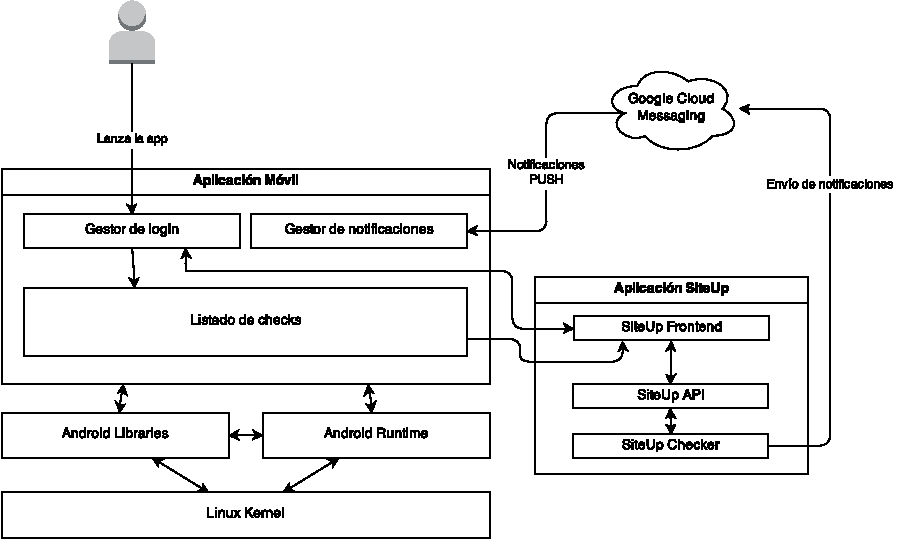
\includegraphics[width=\textwidth]{5_diseno/diagrama_arquitectura_logica_android}
  \caption{Arquitectura lógica de la aplicación Android}
  \label{fig:arquitectura-logica-android}
\end{figure}

En la figura~\ref{fig:arquitectura-logica-android} se puede ver un esquema
general de la arquitectura de la aplicación móvil desarrollada para el sistema
operativo Android. El flujo se detalla a continuación:

\paragraph{Lanzador}

Partimos de la premisa de que el usuario ha instalado la aplicación
\textit{SiteUp Client} en su dispositivo. Si el usuario decide lanzar la
aplicación, deberá dirigirse al lanzador de aplicaciones de su dispositivo y
pulsar sobre el icono de la aplicación, con lo que se iniciará la ejecución.

\paragraph{Gestor de inicio de sesión}

Cuando la aplicación Android se inicia, se lanza una actividad
\texttt{LoginActivity} que hace varias cosas. En primer lugar, verifica si hay
datos de inicio de sesión guardados en el dispositivo. Si no los hay, muestra un
formulario para que el usuario introduzca su nombre de usuario y contraseña. 

Una vez obtenidos los datos, la aplicación móvil se comunica con la plataforma
web para verificar el inicio de sesión. En caso correcto, la plataforma web
envía la información de los chequeos a la aplicación móvil.

\paragraph{Listado de chequeos}

En la aplicación móvil se ha dispuesto una actividad \texttt{CheckListActivity}
que mostrará la lista de chequeos que el usuario ha dado de alta, con
información básica de cada uno de ellos. Cuando el usuario pulse en cualquiera
de los chequeos, se abrirá un navegador y será redirigido a la plataforma web,
particularmente a la página de detalle del chequeo seleccionado.

\paragraph{Gestor de notificaciones}

La aplicación móvil cuenta con un servicio capaz de recibir notificaciones
\textit{Push} del servicio \textit{Google Cloud Messaging}. Cuando se recibe un
mensaje, se muestra una notificación al usuario, informándole también de forma
audible y a través de vibración. La notificación aparece en el área de
notificaciones del sistema operativo. Si el usuario pulsa en la notificación
podrá obtener información sobre el chequeo involucrado.

\paragraph{Google Cloud Messaging}

GCM~\cite{gcm} es un servicio para Android que permite enviar datos desde un
servidor a los dispositivos Android que tengan instaladas una aplicación en
particular. El servicio GCM se encarga de todos los aspectos de la entrega de
mensajes. Se trata de un servicio gratuito independientemente del número de
mensajes y el tamaño de éstos.

GCM recibirá las notificaciones del \textit{backend} de la plataforma móvil, y
se encargará de reenviarlas a los dispositivos Android.

\paragraph{SiteUp Checker}

Dentro de la aplicación móvil, el módulo \texttt{siteup\_checker} es el
encargado de realizar los chequeos, y también de enviar las notificaciones a los
dispositivos Android a través del servicio GCM. La plataforma web tiene una
clave especial con la que se realizan las peticiones a los servidores de Google,
enviando los mensajes.

\paragraph{Runtime y bibliotecas de Android}

Las aplicaciones Android utilizan como base el runtime y las bibliotecas que
provee el sistema operativo para acceder a las funciones del dispositivo y demás
servicios, como la comunicación por red, acceso a datos del usuario, lectura y
escritura de ficheros en el dispositivo, etcétera.


\section{Diseño físico de datos}
\label{sec:diseno-fisico-datos}

En la figura~\ref{fig:diagrama-modelos} se muestra el diagrama de modelos que se
reflejará en la base de datos, donde se puede apreciar cada una de las tablas
que forman el proyecto, así como los campos de las tablas y las relaciones entre
ellas.

\begin{figure}[htbp]
  \centering
  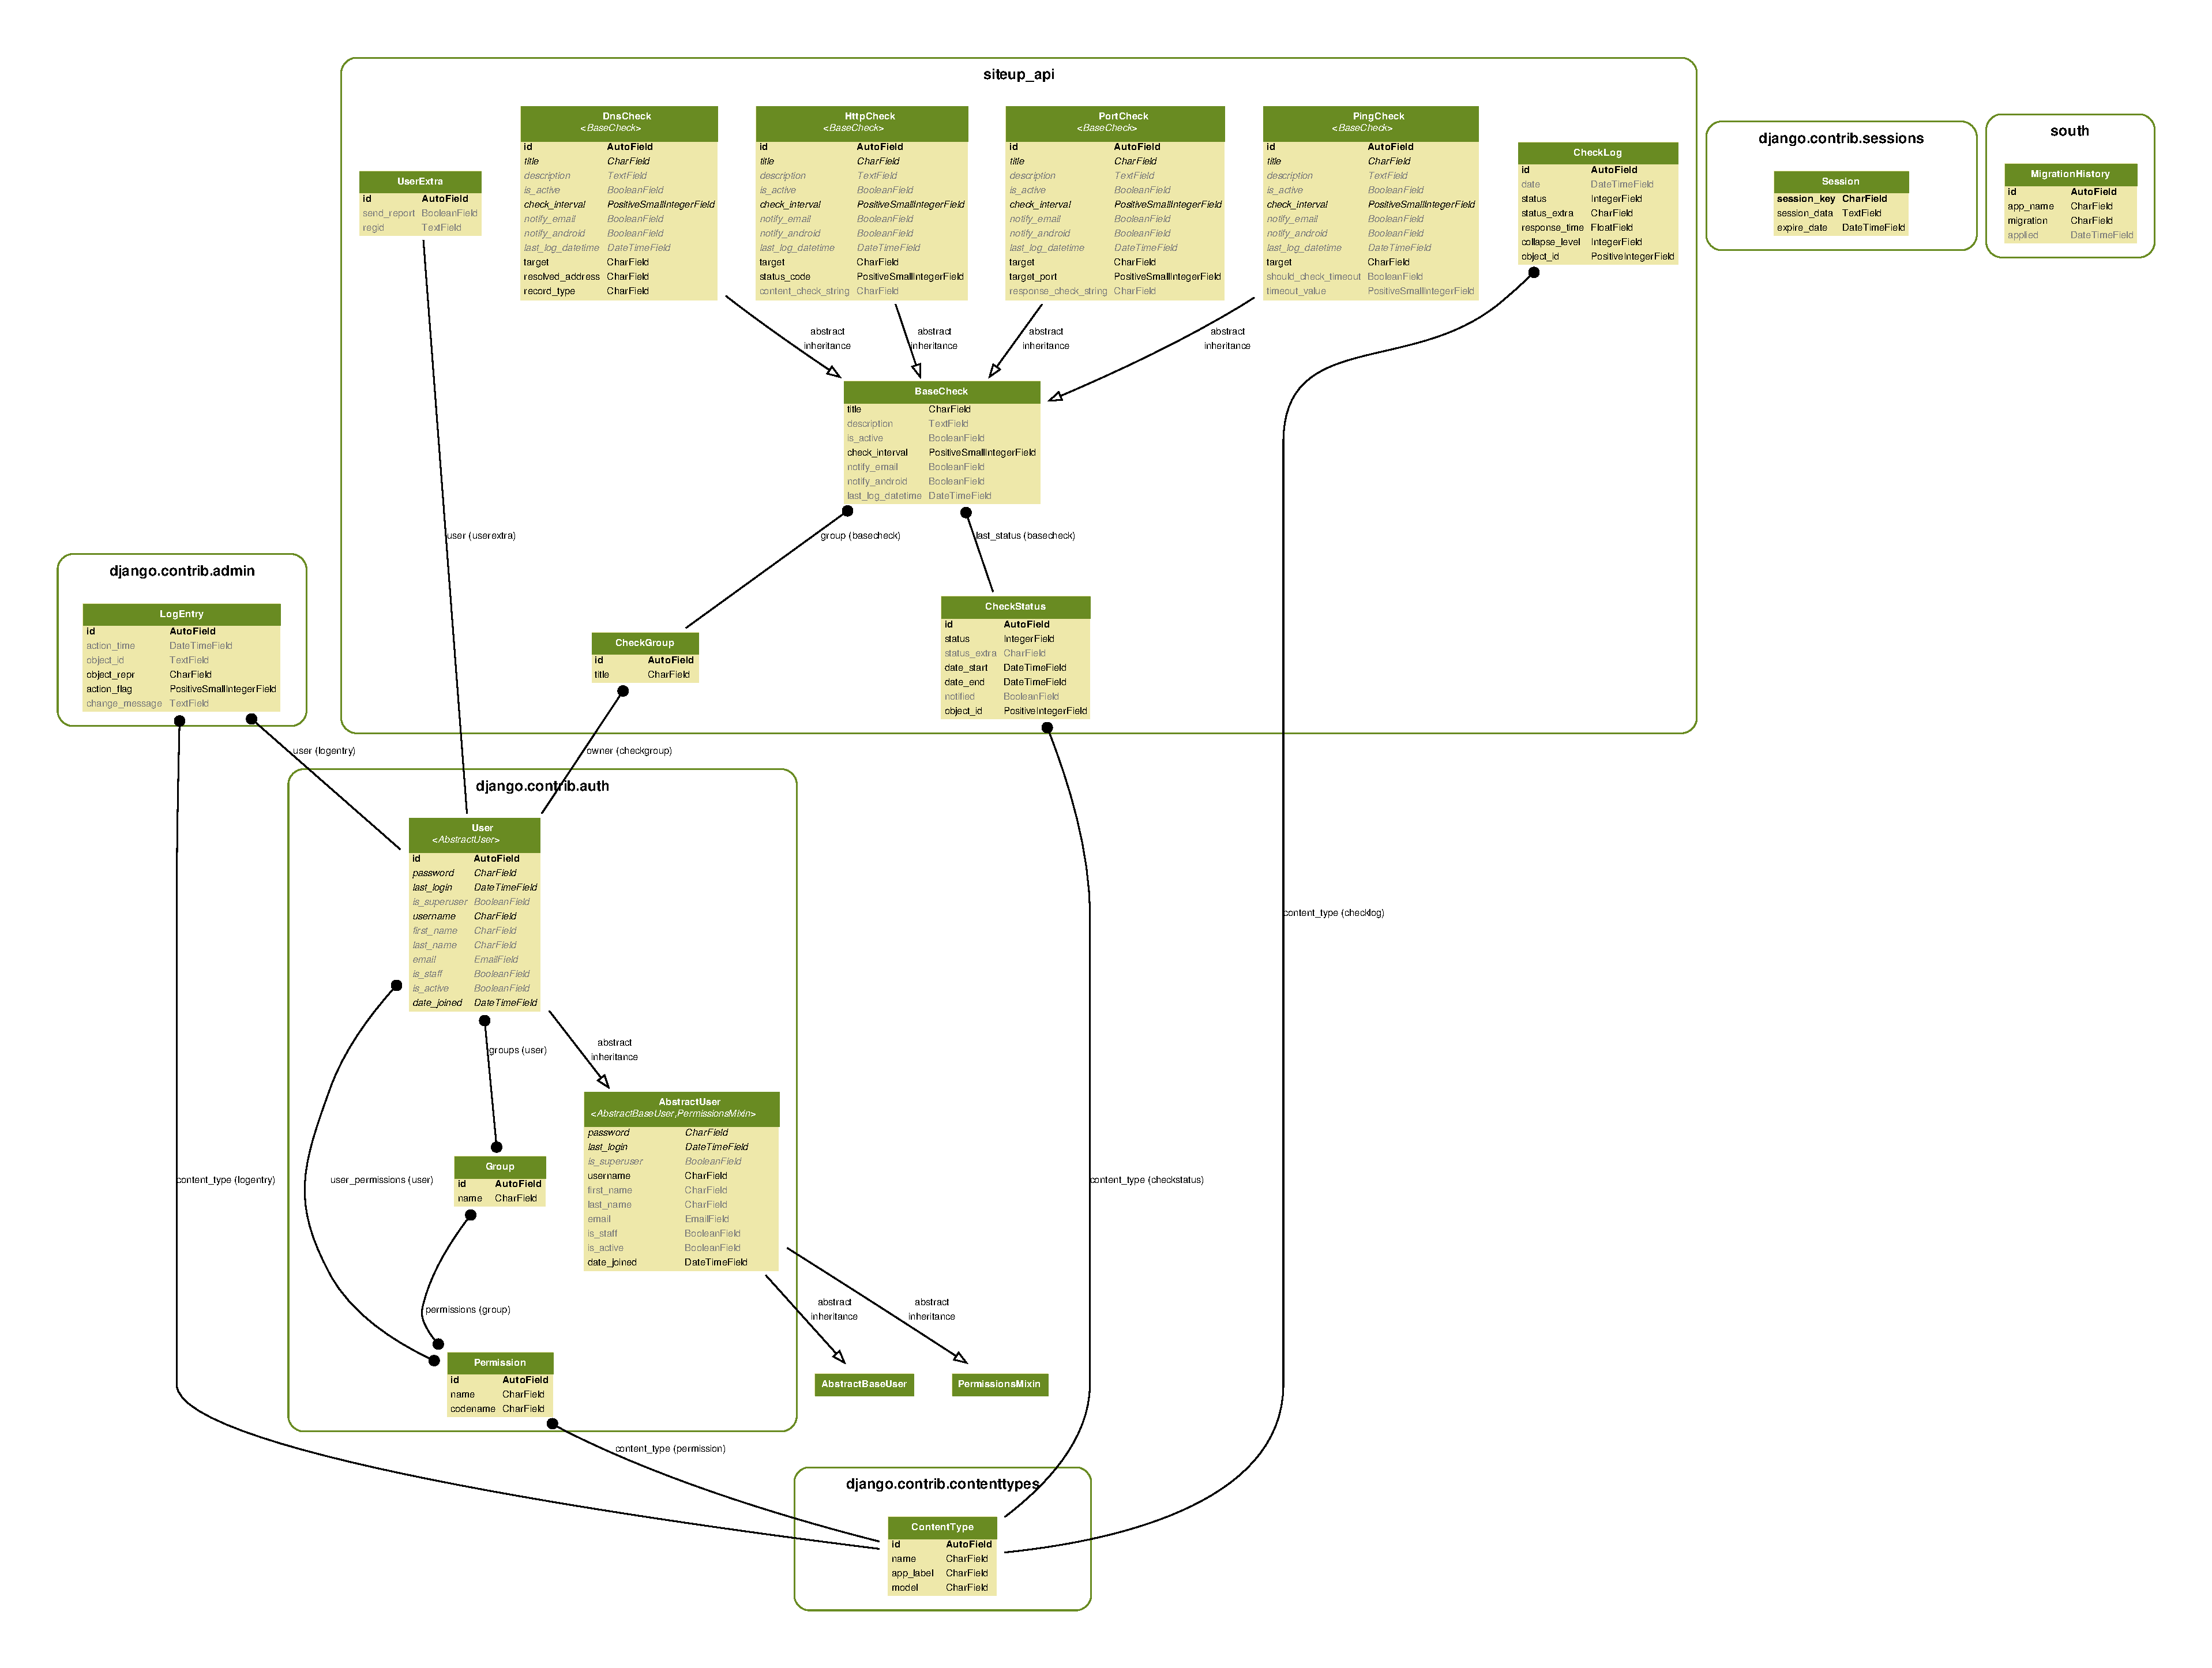
\includegraphics[angle=90, width=\textwidth]{5_diseno/diagrama-modelos}
  \caption{Diseño de la base de datos}
  \label{fig:diagrama-modelos}
\end{figure}

El diseño de los datos se ha hecho mediante las herramientas de mapeo
objeto-relacional que ofrece el framework Django. A continuación se detallan los
principales modelos con los que cuenta el sistema.

\subsection{User}

Este modelo representa a un usuario registrado en el sistema. Es un modelo
predeterminado de Django y forma parte de la aplicación \texttt{django.contrib.auth}.

Sus principales campos son:

\begin{itemize}
\item \texttt{username} - Nombre de usuario.
\item \texttt{password} - Contraseña. Se almacena en forma de cifrado
  irreversible de acuerdo a las exigencias de la actual Ley de Protección de Datos.
\item \texttt{email} - Dirección de correo electrónico.
\end{itemize}

\subsection{UserExtra}

Este modelo guarda información adicional sobre los usuarios, evitando así tener
que modificar el modelo que integra Django. Forma parte de la aplicación \texttt{siteup\_api}.

Sus principales campos son:

\begin{itemize}
\item \texttt{send\_report} - Booleano, indica si el usuario recibirá reportes
  diarios sobre el estado de sus chequeos.
\item \texttt{regid} - Texto, guarda el identificador único del dispositivo
  Android obtenido a través de Google Play Services.
\end{itemize}

\subsection{CheckGroup}

Parte de la aplicación \texttt{siteup\_api}. Identifica a un grupo de
chequeos. Todos los chequeos deben pertenecer a un grupo. 

El campo principal de este modelo es \texttt{title}, que guarda una cadena con
el título del grupo.

\subsection{BaseCheck}

Parte de la aplicación \texttt{siteup\_api}. Este modelo \textbf{abstracto}
guarda campos comunes a todos los tipos de chequeos. No tiene representación
directa en la base de datos, sino que sirve para evitar duplicidad de código.

Sus principales campos son:

\begin{itemize}
\item \texttt{title} - Texto, representa el título del chequeo.
\item \texttt{description} - Texto, representa la descripción del chequeo.
\item \texttt{is\_active} - Booleano, indica si el chequeo está activo.
\item \texttt{check\_interval} - Entero, indica el intervalo entre chequeos en minutos.
\item \texttt{notify\_email} - Booleano, indica si los cambios de estado del
  chequeo se notificarán vía correo electrónico.
\item \texttt{notify\_android} - Booleano, indica si los cambios de estado del
  chequeo se notificarán vía Android utilizando notificaciones push.
\item \texttt{last\_log\_datetime} - Fecha, almacena la fecha de la última vez que se lanzó el chequeo.
\end{itemize}

\subsection{DnsCheck}

Parte de la aplicación \texttt{siteup\_api}. Este modelo deriva de
\texttt{BaseCheck} y representa un chequeo de registros DNS. Sus principales campos son:

\begin{itemize}
\item \texttt{target} - Texto, indica el dominio a chequear.
\item \texttt{record\_type} - Enum, indica el tipo de registro a chequear. Puede ser de tipo A, AAAA, CNAME, MX y TXT.
\item \texttt{resolved\_address} - Texto, indica el contenido que debe tener el registro revisado.
\end{itemize}

\subsection{HttpCheck}

Parte de la aplicación \texttt{siteup\_api}. Este modelo deriva de
\texttt{BaseCheck} y representa un chequeo a través de peticiones HTTP.

Sus principales campos son:

\begin{itemize}
\item \texttt{target} - Texto, indica la URL a comprobar.
\item \texttt{status\_code} - Entero, indica el código de estado que se debe recibir.
\item \texttt{content\_check\_string} - Cadena, representa una cadena de texto
  que, opcionalmente, debe estar presente en la respuesta obtenida desde la URL indicada.
\end{itemize}

\subsection{PortCheck}

Parte de la aplicación \texttt{siteup\_api}. Este modelo deriva de
\texttt{BaseCheck} y representa un chequeo de puertos remotos.

Sus principales campos son:

\begin{itemize}
\item \texttt{target} - Cadena, identifica el servidor remoto al que conectarse.
\item \texttt{target\_port} - Entero, indica el puerto remoto al que conectarse.
\item \texttt{response\_check\_string} - Cadena, representa una cadena de texto
  que, opcionalmente, debe estar presente en la respuesta obtenida desde el servidor.
\end{itemize}

\subsection{PingCheck}

Parte de la aplicación \texttt{siteup\_api}. Este modelo deriva de
\texttt{BaseCheck} y representa un chequeo mediante el envío de paquetes \ac{ICMP}.

Sus principales campos son:

\begin{itemize}
\item \texttt{target} - Cadena, identifica al servidor remoto que hay que chequear.
\item \texttt{should\_check\_timeout} - Booleano, indica si hay que comprobar el tiempo de respuesta de los paquetes ping.
\item \texttt{timeout\_value} - Entero, si el anterior campo evalúa a
  \textit{Verdadero}, este campo guarda el tiempo de respuesta máximo permitido.
\end{itemize}

\subsection{CheckLog}

Parte de la aplicación \texttt{siteup\_api}. Es un registro (\textit{log}) que
representa el resultado de ejecutar un chequeo.

Sus principales campos son:

\begin{itemize}
\item \texttt{date} - Fecha, representa el momento en el que se obtuvo el resultado.
\item \texttt{status} - Entero, representa el estado del chequeo que se ha
  obtenido. Los posibles valores son:
  \begin{itemize}
  \item 0: el chequeo ha terminado correctamente y el estado es correcto (\textit{Up}).
  \item 1: el chequeo ha terminado correctamente y el estado es negativo (\textit{Down}).
  \item 2: el chequeo no ha podido concluirse. Equivalente en estadísticas al estado negativo. (\textit{Error}).
  \end{itemize}
\item \texttt{response\_time} - Entero, solo válido para los chequeos de tipo
  Ping. Guarda el tiempo de respuesta obtenido.
\item \texttt{collapse\_level} - Entero. Indica el nivel de \textit{colapsado}
  del registro. Dado que el número de registros es muy alto (en una hora pueden
  llegar a generarse más de 3600 registros por chequeo), es necesario resumir
  los registros más antiguos. Este campo indica si el \textit{CheckLog} ya ha
  sido resumido o no.
\end{itemize}

\subsection{CheckStatus}

Parte de la aplicación \texttt{siteup\_api}. Representa un cambio de estado de
un chequeo. Cuando un chequeo es ejecutado, se genera una instancia de
\textit{CheckLog} y se comprueba el estado de éste con el estado de la última
comprobación. Si se verifica que el estado ha cambiado con respecto a los
últimos estados, se genera una instancia de \textit{CheckStatus} y se lanzan las
notificaciones pertinentes.

Los campos principales de este modelo son:

\begin{itemize}
\item \texttt{status} - Entero, indica el estado. El código numérico responde al
  mismo formato que se sigue en el modelo \textit{CheckLog}.
\item \texttt{status\_extra} - Cadena, guarda información adicional sobre el estado.
\item \texttt{date\_start} - Fecha, indica el momento en el que el chequeo
  cambia a este estado.
\item \texttt{date\_end} - Fecha, indica el momento en el que el chequeo deja de
  estar en este estado. Si es el estado actual de un chequeo, se mantiene en blanco.
\item \texttt{notified} - Booleano, indica si este cambio de estado ha sido ya notificado.

\end{itemize}

\subsection{Session}

Parte de la aplicación \texttt{django.contrib.sessions}. Representa una sesión
de usuario en la aplicación web. Sus campos principales son:

\begin{itemize}
\item \texttt{session\_key} - Cadena, guarda el identificador de la sesión.
\item \texttt{session\_data} - Texto, guarda los datos asociados a la sesión.
\item \texttt{expire\_date} - Fecha, indica hasta qué fecha son válidos los
  datos de la sesión.
\end{itemize}

\subsection{MigrationHistory}

Parte de la aplicación \texttt{south}. Representa una migración de la base de
datos. Los campos principales son:

\begin{itemize}
\item \texttt{app\_name} - Cadena, nombre de la app sobre la que se ahce la migración.
\item \texttt{migration} - Cadena, identificador de la migración.
\item \texttt{applied} - Fecha, indica cuándo se aplicó la migración.
\end{itemize}

\subsection{ContentType}

Parte de la aplicación \texttt{django.contrib.contenttypes}. Es el bloque
principal del \textit{Content Types Framework}, un framework integrado en Django
que permite trabajar de forma genérica con los modelos, ofreciendo
funcionalidades como la posibilidad de crear claves foráneas genéricas (es
decir, que puedan apuntar a cualquier modelo. 

Una instancia de \textit{ContentType} representa un modelo particular de una
aplicación en concreto. Los campos que contiene son:

\begin{itemize}
\item \texttt{name} - Cadena, nombre del modelo en formato legible.
\item \texttt{model} - Cadena, nombre original del modelo.
\item \texttt{app\_label} - Cadena, nombre de la aplicación a la que pertence el
  módulo.
\end{itemize}

\section{Diseño de la imagen corporativa}

La \textbf{imagen corporativa} del proyecto comprende el diseño del
\textbf{logotipo}, la elección de la paleta de \textbf{colores} y las
\textbf{tipografías}, que se usan en el diseño de la web, emails y cualquier
otro elemento visual.

Para su elaboración se han seguido ciertas premisas o \textit{guías de
  branding}, de forma que se consiguiese el look más adecuado:

\begin{itemize}
\item \textbf{Diseño minimalista}. En SiteUp, la información es lo más
  importante, así que no tiene sentido utilizar un diseño muy sobrecargado.
\item \textbf{Colores monocromáticos}. Siguiendo en la línea del punto anterior,
  esta \textit{regla} facilita que haya una consistencia en las interfaces de la
  web y la aplicación móvil sin tener que recurrir a complejas combinaciones de
  color.
\item \textbf{Tipografías libres}. Era importante no utilizar tipografías que
  requiriesen una licencia comercial para su uso.
\end{itemize}

\subsection{Diseño del logotipo}
\label{subsec:logotipo}

Partiendo del nombre del proyecto se pensaron varios bocetos para el
logotipo. La idea principal era jugar con las dos palabras que componen el
nombre: \textit{Site} y \textit{Up}. Para la primera palabra, la metáfora de
usar una ventana de un navegador o algo que representase un servidor era
demasiado compleja, así que se decidió simplemente usar la letra S. 

Por otro lado, para la segunda palabra estaba claro desde el principio que se
usaría alguna metáfora de tipo flecha para representar la dirección
\textit{arriba}. Se probaron distintos tipos de flechas y al final se decidió
por una doble flecha de tipo galón, con suficiente separación para que se viese
en bajas resoluciones. El logotipo resultante se puede ver en la
figura~\ref{fig:logotipo}

\begin{figure}[H]
  \centering
  
\includegraphics[width=0.5\textwidth]{5_diseno/logo.png}
  \caption{Logotipo de SiteUp}
  \label{fig:logotipo}
\end{figure}

\subsection{Elección de la gama cromática}

Teniendo en mente la idea apuntada anteriormente de que la gama de colores
debería ser preferiblemente monocromática, se empezó a buscar un tono que
funcionase con la temática del sitio. Se hizo una búsqueda de sitios web de
servicios de soporte, y en la mayoría de ellos la gama cromática era siempre muy
neutra, con tonos poco saturados y casi siempre fríos.

\begin{figure}[H]
  \centering
  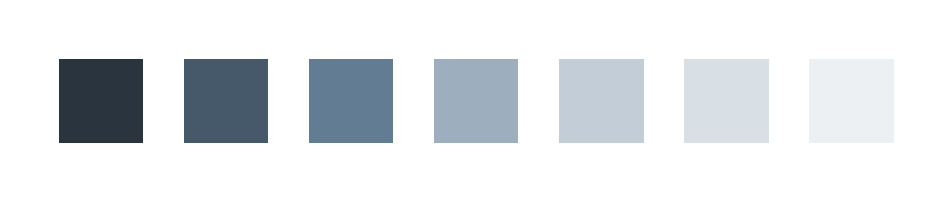
\includegraphics[width=\textwidth]{5_diseno/paleta-colores}
  \caption{Detalle de la paleta de colores de SiteUp}
  \label{fig:colores}
\end{figure}

Así, tras varias pruebas, se decidió optar por una gama de azules poco
saturados, rozando el grisáceo. En la figura~\ref{fig:colores} se detalla la
paleta de colores principal.

\subsection{Elección de la tipografía}

Siguiendo las directrices apuntadas previamente, se buscaba una tipografía
sencilla y minimalista. Se probaron algunas alternativas comerciales, empezando,
cómo no, por Helvética y pasando por Myriad Pro, Próxima Nova y algunas
otras. Al final nos decantamos por utilizar \textbf{Open Sans}~\cite{open-sans},
una tipografía sans-serif limpia y moderna, de corte humanista, y desarrollada
por Steve Matteson para Google.

Se trata de una tipografía limpia, optimizada para la legibilidad en toda clase
de soportes, y por supuesto libre, bajo una licencia Apache 2.0.

\begin{figure}[H]
  \centering
  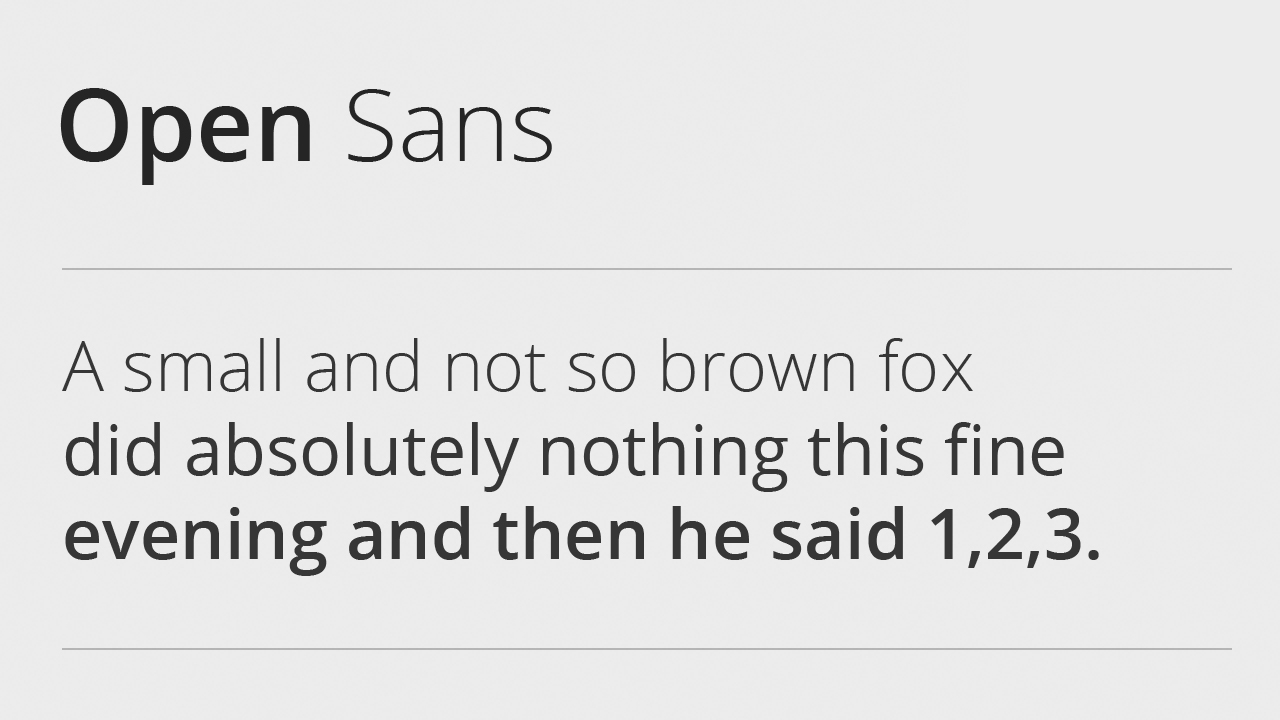
\includegraphics[width=0.8\textwidth]{5_diseno/open-sans}
  \caption{Muestra de Open Sans en diferentes pesos}
\end{figure}

\section{Diseño de la interfaz de usuario de la plataforma web}

En esta sección se detallarán las interfaces visuales de la plataforma web del
proyecto, indicando qué acciones realizan cada uno de los componentes que las
conforman.

\subsection{Pantalla de inicio}

\begin{figure}[htbp]
  \centering
  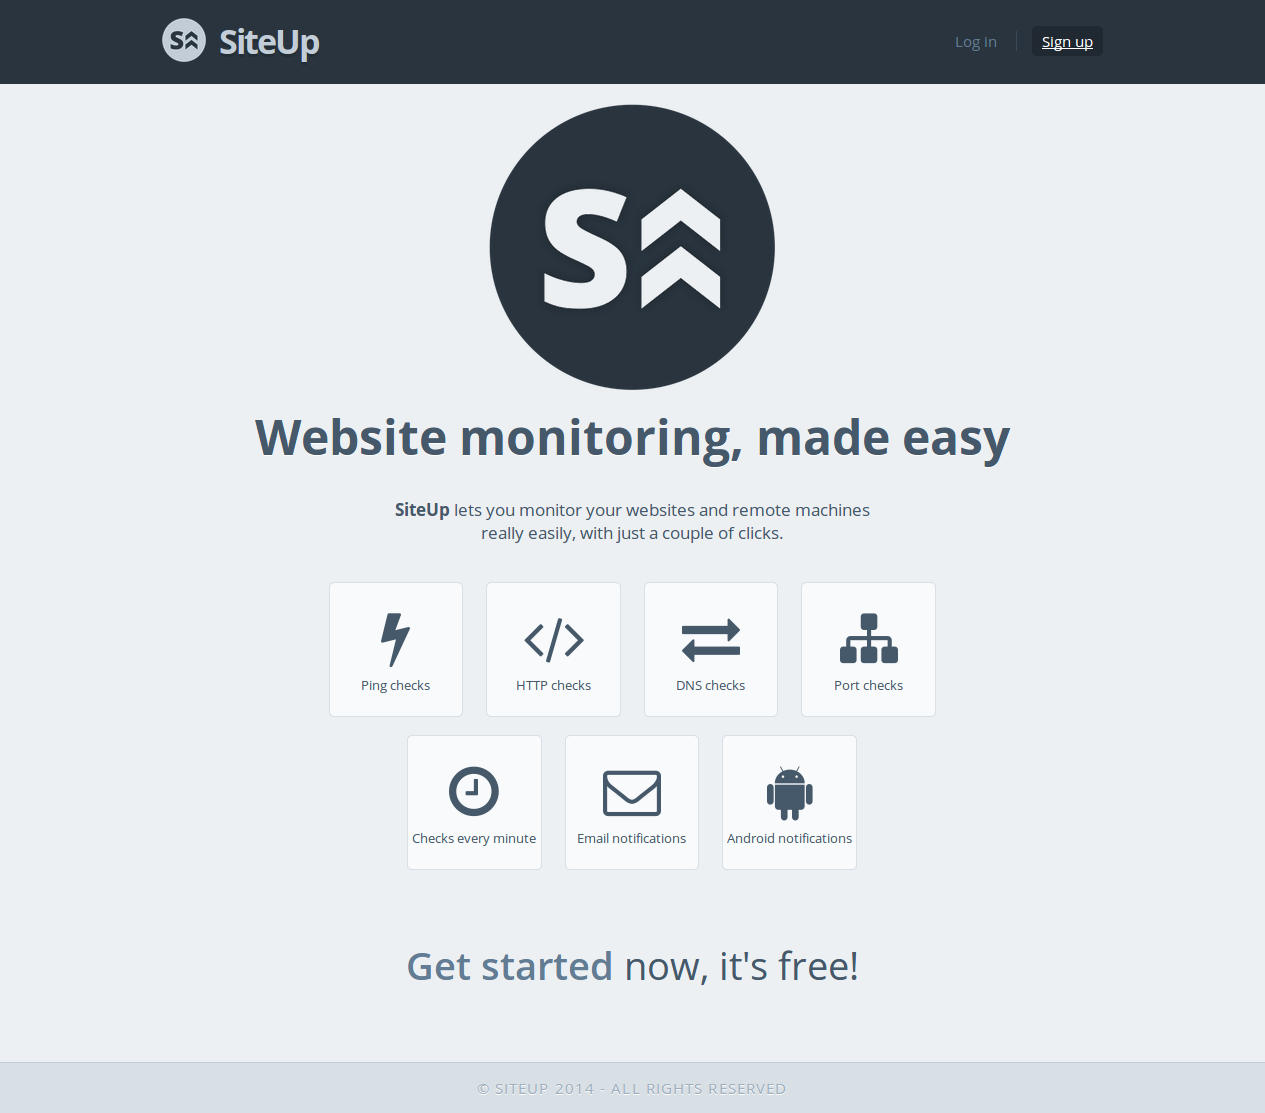
\includegraphics[width=\textwidth]{5_diseno/web-home.png}
  \caption{Pantalla de inicio}
  \label{fig:web-home}
\end{figure}

En la figura~\ref{fig:web-home} se ve el diseño de página de inicio, o
\textit{home}, de la plataforma web. Es la pantalla que aparece al acceder a la
base del proyecto. Se componen de una barra superior de navegación en la que
aparece el logotipo a la izquierda, y las opciones de navegación a la
derecha. Al pulsar el logotipo, se redirige a la pantalla de inicio.

Si el usuario no está logueado, las opciones de navegación disponibles son:

\begin{itemize}
\item \textbf{Log in}: lleva al usuario a la pantalla de inicio de sesión.
\item \textbf{Sign up}: lleva al usuario a la pantalla de registro de usuario.
\end{itemize}

Si el usuario sí está logueado, las opciones que aparecen son diferentes:

\begin{itemize}
\item \textbf{Dashboard}: lleva al usuario al listado de chequeos.
\item \textbf{Your profile}: lleva al usuario al formulario de datos personales.
\item \textbf{Log out}: cierra la sesión del usuario.
\end{itemize}

La barra de navegación superior tiene el mismo comportamiento en todas las
secciones de la web.


\subsection{Pantalla de inicio de sesión}

\begin{figure}[htbp]
  \centering
  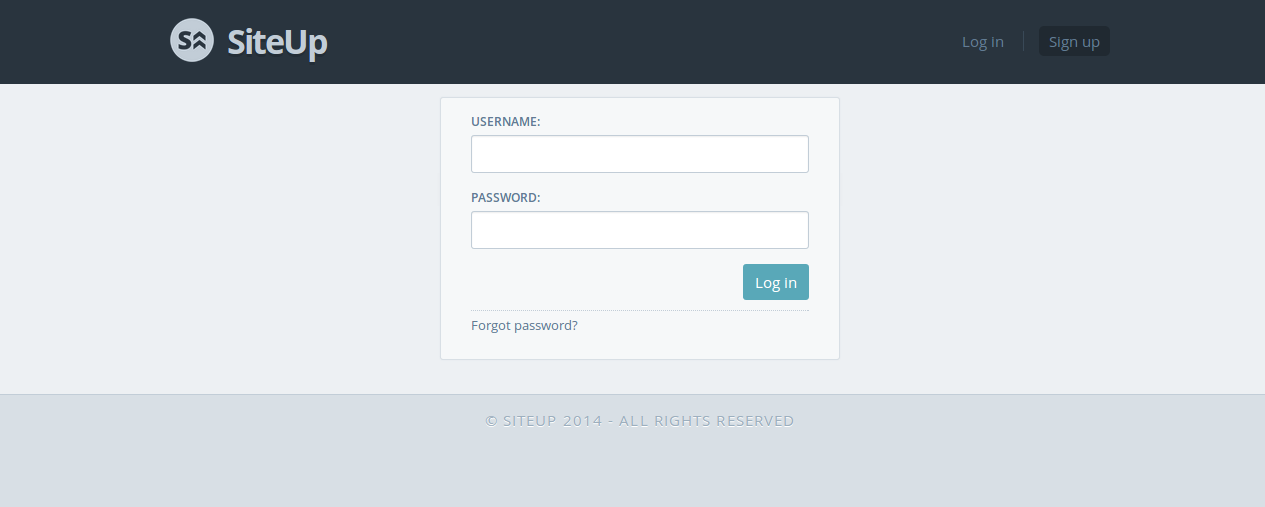
\includegraphics[width=\textwidth]{5_diseno/web-login.png}
  \caption{Pantalla de inicio de sesión}
  \label{fig:web-login}
\end{figure}

En la figura~\ref{fig:web-login} se ve el diseño de la pantalla de inicio de
sesión. Se presenta un formulario en el que el usuario deberá escribir su nombre
de usuario y su contraseña, y tras ello pulsar el botón de \textit{Login}. En
caso de que los datos introducidos sean correctos, el sistema iniciará sesión y
redirigirá al usuario a la lista de chequeos. En caso contrario, volverá a
aparecer el formulario con los errores que se hayan producido.

Opcionalmente, si el usuario no recuerda su contraseña puede pulsar en el botón
de \textit{Forgot password?}, lo que le llevará a la pantalla de recuperación de
contraseña.

\subsection{Pantalla de recuperación de contraseña}

\begin{figure}[htbp]
  \centering
  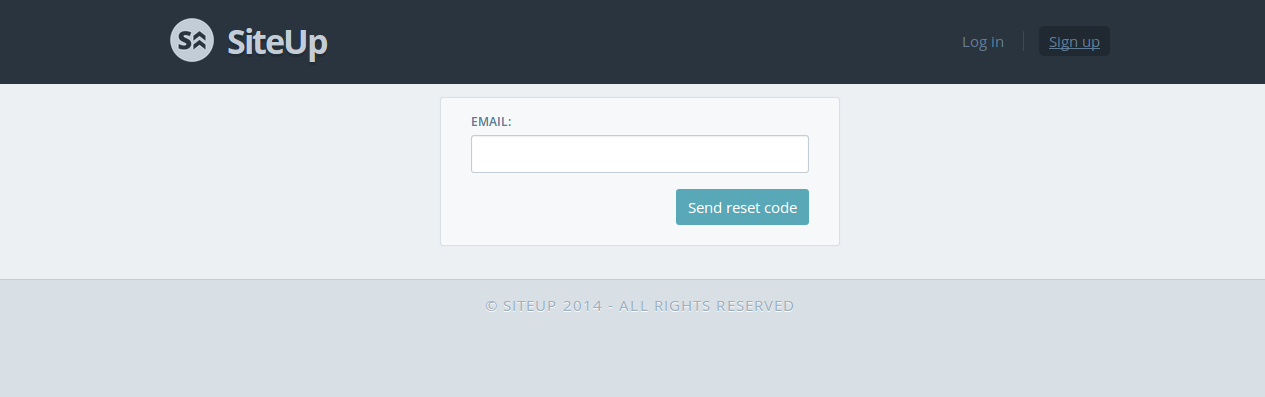
\includegraphics[width=\textwidth]{5_diseno/web-forgot-password}
  \caption{Pantalla de recuperación de contraseña}
  \label{fig:web-forgot-password}
\end{figure}

En esta pantalla, visible en la figura~\ref{fig:web-forgot-password}, el usuario
podrá introducir su correo electrónico para recuperar su contraseña. Tras
rellenar el campo de texto, deberá pulsar el botón. Si el email introducido es
correcto, el sistema enviará un correo electrónico con instrucciones para
reiniciar la contraseña, y en pantalla se mostrará un mensaje indicando que se
ha iniciado el proceso de reinicio.

% \vfill

\subsection{Pantalla de registro de usuario}

En la figura~\ref{fig:web-register} se puede ver la pantalla de registro de
usuario.

\begin{figure}[htbp]
  \centering
  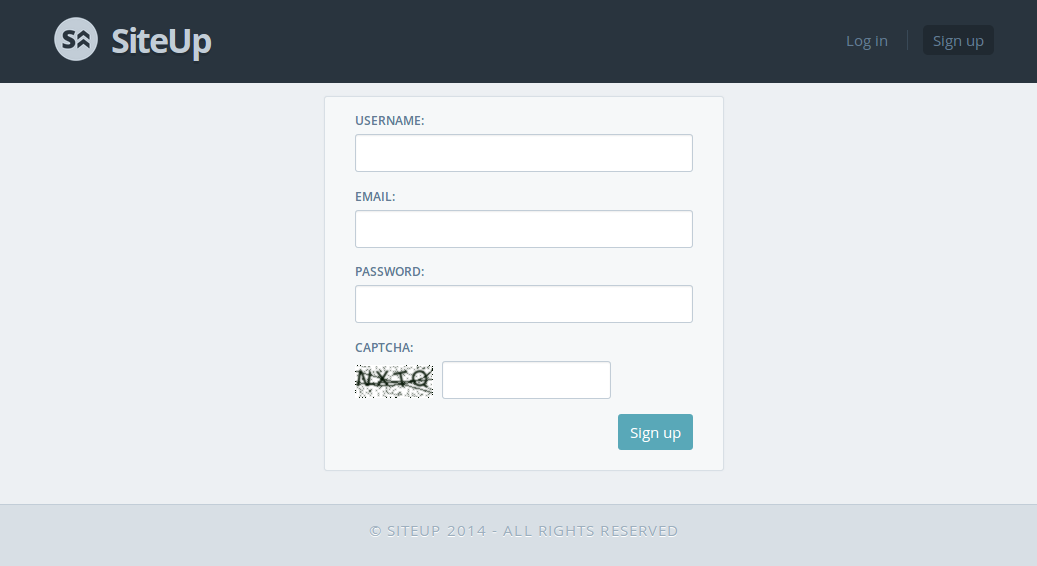
\includegraphics[width=\textwidth]{5_diseno/web-register}
  \caption{Pantalla de registro de usuario}
  \label{fig:web-register}
\end{figure}

Dispone de un formulario, en el que el usuario deberá introducir sus datos
personales: nombre de usuario, dirección de correo electrónico y contraseña. Una
vez rellenos, deberá pulsar el botón. Si los datos son correctos, el sistema
creará la cuenta de usuario. Si no, el sistema volverá a mostrar el formulario,
resaltando los errores en los datos.

% \vfill

\subsection{Pantalla de lista de chequeos}

\begin{figure}[htbp]
  \centering
  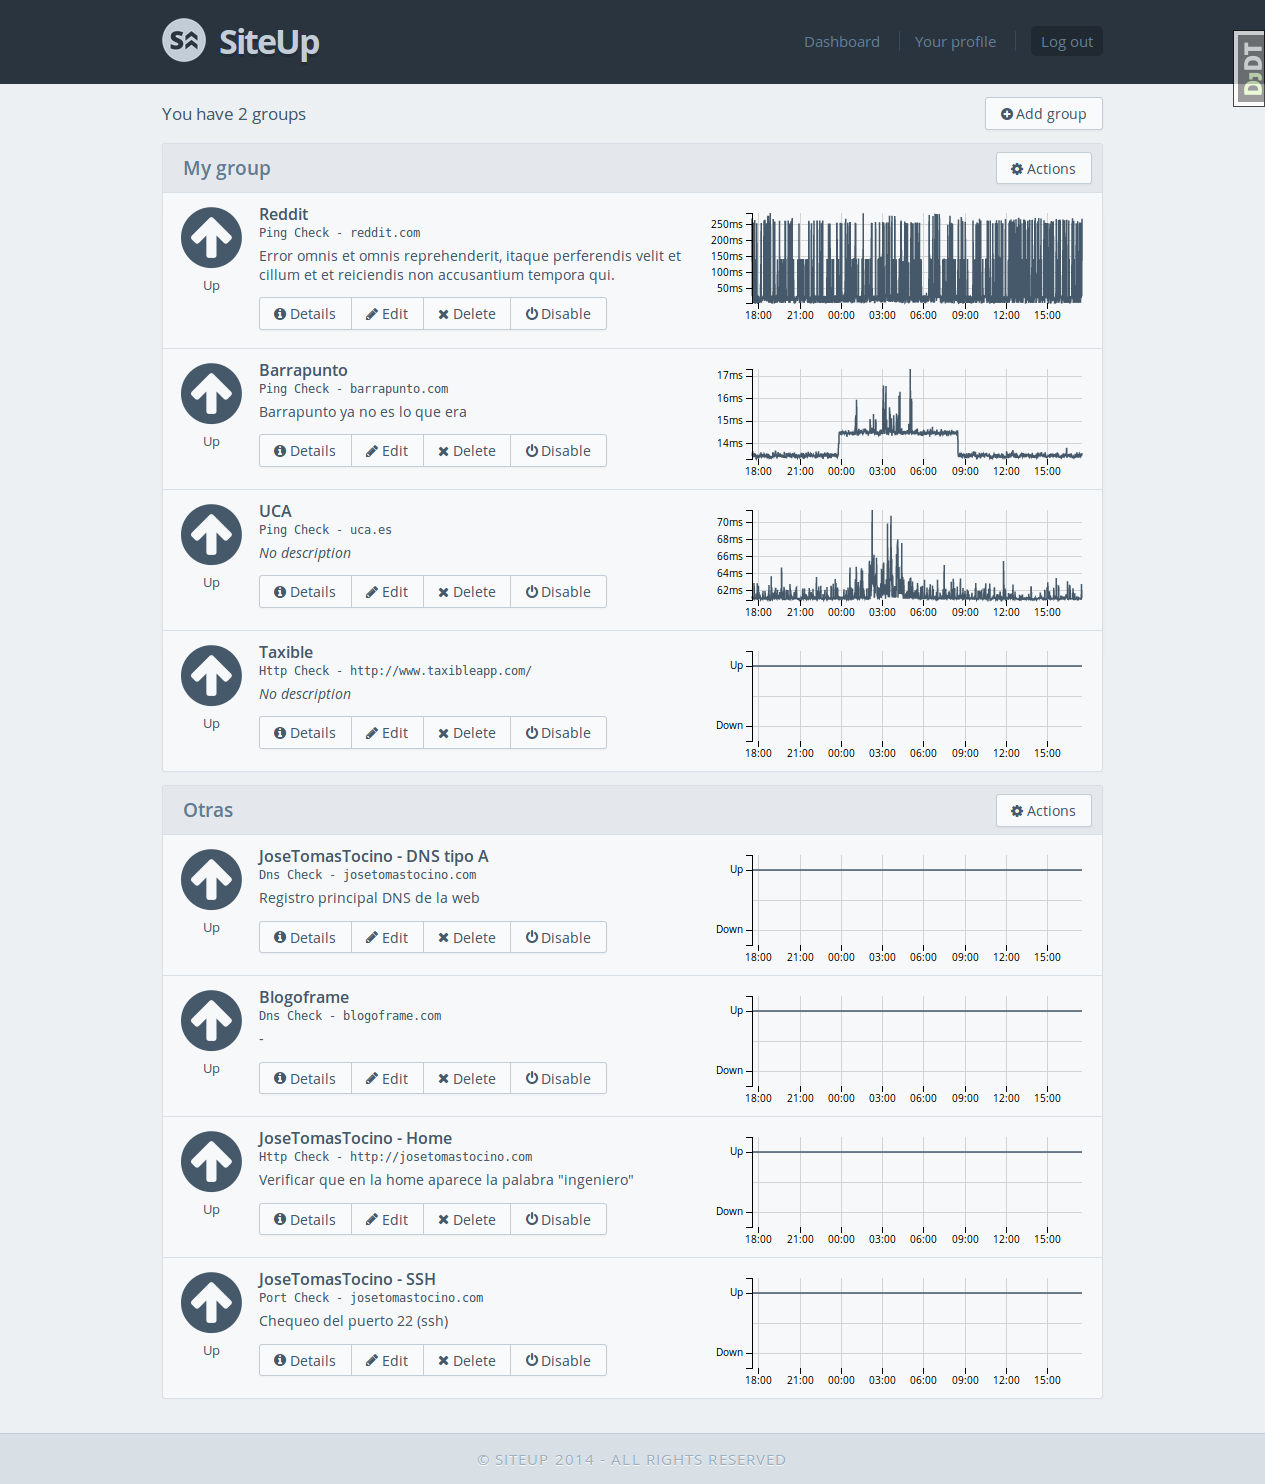
\includegraphics[width=\textwidth]{5_diseno/web-dashboard}
  \caption{Pantalla de lista de chequeos}
  \label{fig:web-dashboard}
\end{figure}

En la figura~\ref{fig:web-dashboard} se puede ver la pantalla principal de
SiteUp, la lista de chequeos o \textbf{dashboard}. En esta pantalla aparecen los
grupos de chequeos que tiene dados de alta un usuario, así como los chequeos que
pertenecen a cada grupo. Desde esta pantalla se pueden hacer un gran número de
operaciones:

\begin{itemize}
\item Pulsando el botón \textit{Add group} aparecerá la pantalla de creación de
  grupo.
\item Cada grupo tiene un menú desplegable que aparece al pulsar o colocar el
  ratón sobre el botón \textit{Actions}. Desde ahí, es posible:
  \begin{itemize}
  \item Añadir un chequeo al grupo pulsando el botón \textit{Add check}.
  \item Activar todos los chequeos del grupo pulsando el botón \textit{Enable
      all checks}.
  \item Desactivar todos los chequeos del grupo pulsando el botón
    \textit{Disable all checks}.
  \item Editar los detalles del grupo pulsando el botón \textit{Edit}.
  \item Borrar el grupo y los chequeos que contiene pulsando el botón \textit{Delete}.
  \end{itemize}
\item Dentro de cada grupo aparece cada uno de los chequeos que contiene, con un
  icono indicando el estado del chequeo, el título, descripción, una gráfica de
  su estado en las últimas 24 horas y una serie de botones de acción, que
  permiten:
  \begin{itemize}
  \item Ver los detalles del chequeo pulsando el botón \textit{Details}.
  \item Editar las propiedades del chequeo con el botón \textit{Edit}.
  \item Borrar el chequeo con el botón \textit{Delete}.
  \item Activar o desactivar el chequeo pulsando \textit{Enable} o
    \textit{Disable}.
  \end{itemize}

\end{itemize}

\subsection{Pantalla de detalles de chequeo}

\begin{figure}[htbp]
  \centering
  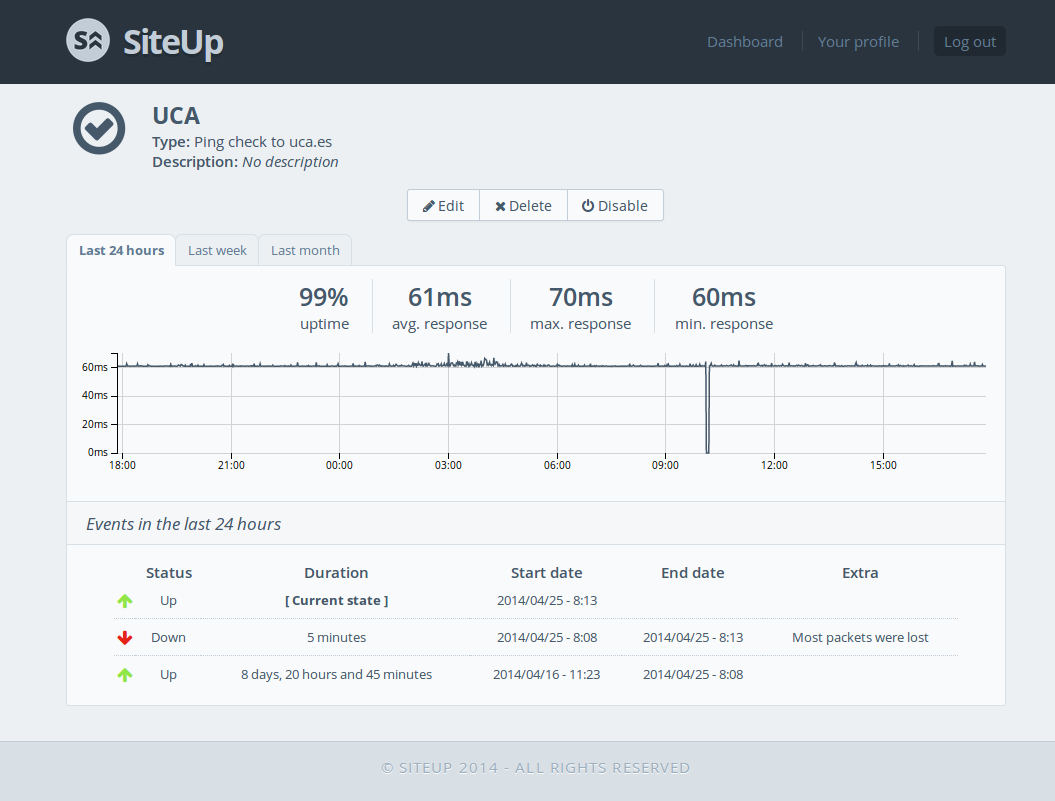
\includegraphics[width=\textwidth]{5_diseno/web-check-detail.png}
  \caption{Pantalla de detalles de chequeo}
  \label{fig:web-check-detail}
\end{figure}

En la figura ~\ref{fig:web-check-detail} se puede ver la pantalla de detalle de
un chequeo, a la que se accede pulsando el botón \textit{details} desde el panel
de control principal. Desde esta pantalla es posible realizar operaciones con el
chequeo (editar, borrar y desactivar), así como ver información y eventos
ocurridos en distintos intervalos de tiempo.

% \vfill

\subsection{Pantalla de creación de grupo}

\begin{figure}[htbp]
  \centering
  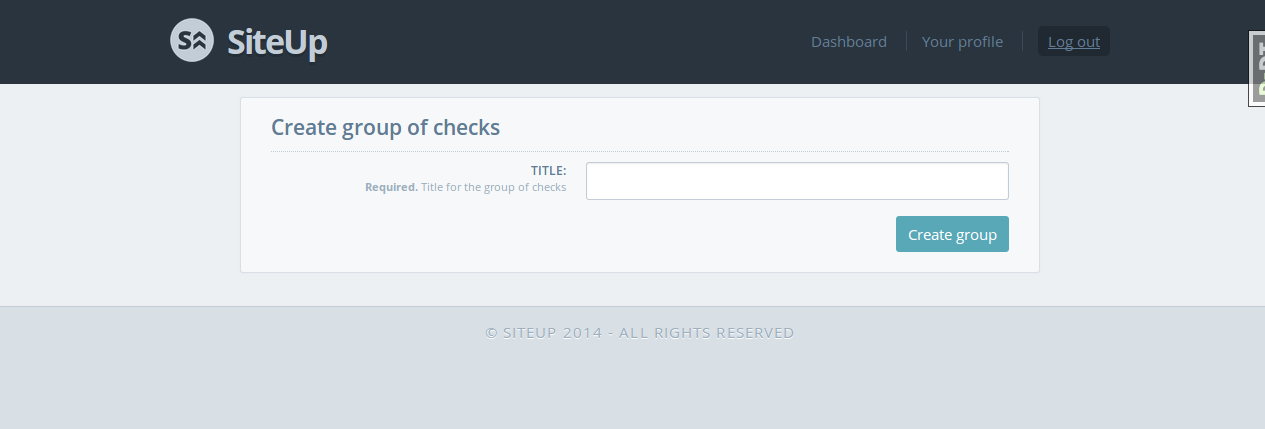
\includegraphics[width=\textwidth]{5_diseno/web-create-group}
  \caption{Pantalla de creación de grupo de chequeos}
  \label{fig:web-create-group}
\end{figure}

La figura~\ref{fig:web-create-group} representa la pantalla para crear un grupo
de chequeos. Muestra un formulario en el que hay que introducir los detalles del
grupo, concretamente el título que lo describe.

Cuando el usuario introduzca el título y pulse el botón, el sistema revisará que
los datos sean correctos. En caso afirmativo, el sistema creará el nuevo
grupo. En caso negativo, se volverá a mostrar el formulario, indicando los
fallos ocurridos.

% \vfill

\subsection{Pantallas de creación de chequeo}

\begin{figure}[htbp]
  \centering
  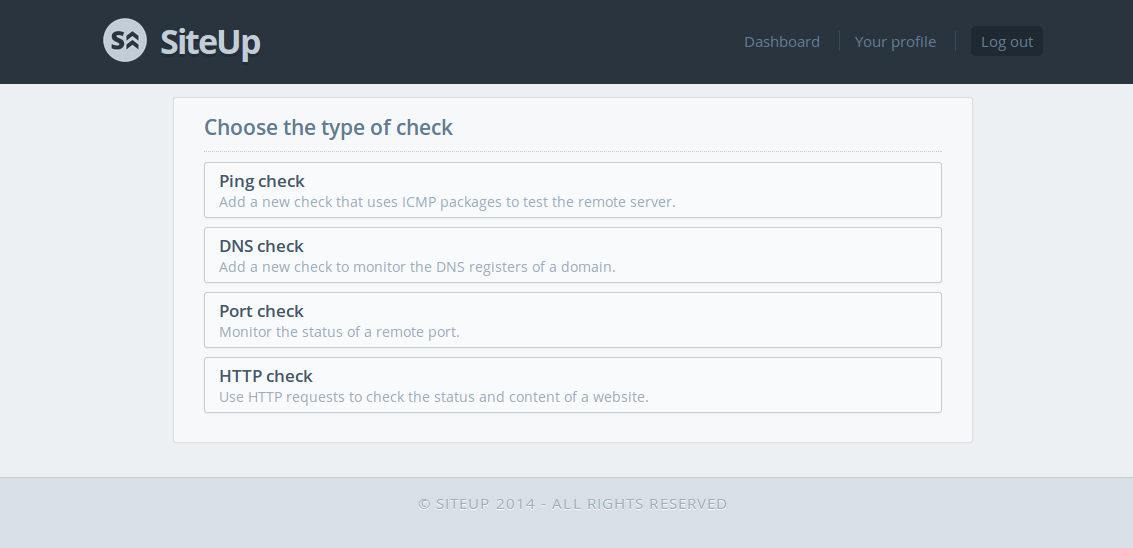
\includegraphics[width=\textwidth]{5_diseno/web-choose-type}
  \caption{Pantalla de elección de tipo de chequeo}
  \label{fig:web-choose-type}
\end{figure}

La creación de un chequeo se divide en dos pantallas principalmente. El primer
paso es elegir el tipo de chequeo a crear, mediante los botones que aparecen en
la pantalla de la figura~\ref{fig:web-choose-type}. 

Una vez elegido el tipo de chequeo a crear, aparecerá un formulario para
introducir los detalles del chequeo, que variará según el tipo de chequeo
elegido. En la figura~\ref{fig:web-create-check} se puede ver el formulario que
aparecerá a la hora de crear un chequeo de tipo DNS.

\begin{figure}[htbp]
  \centering
  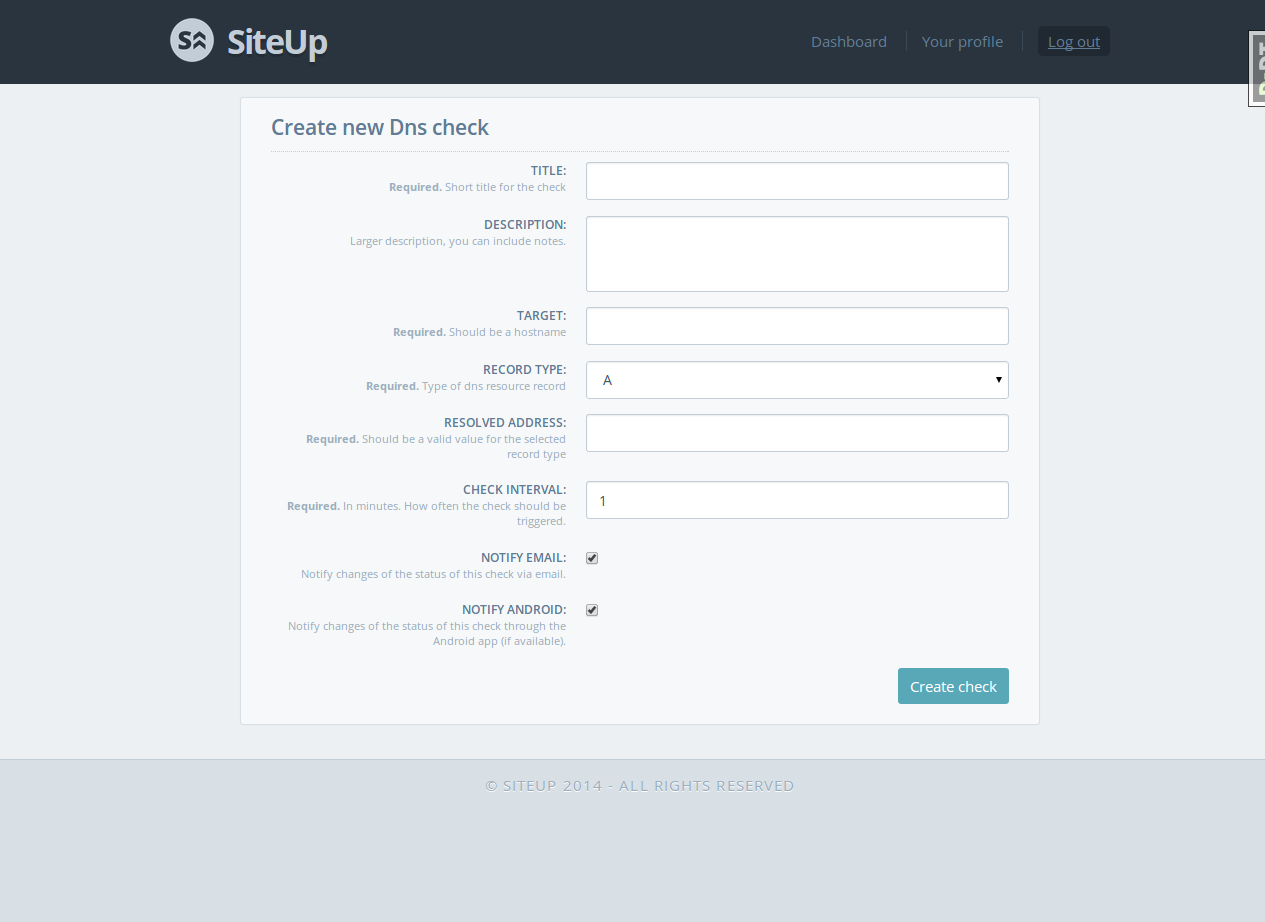
\includegraphics[width=\textwidth]{5_diseno/web-create-check}
  \caption{Pantalla de introducción de datos del chequeo}
  \label{fig:web-create-check}
\end{figure}


Cuando el usuario rellene el formulario y pulse el botón, se enviarán los datos
y el sistema comprobará que la información es correcta. En tal caso, se creará
el nuevo chequeo y se redirigirá al usuario al \textit{dashboard}. En caso
contrario, se volverá a mostrar el formulario, indicando los errores
encontrados.

\subsection{Pantalla genérica de borrado}

\begin{figure}[htbp]
  \centering
  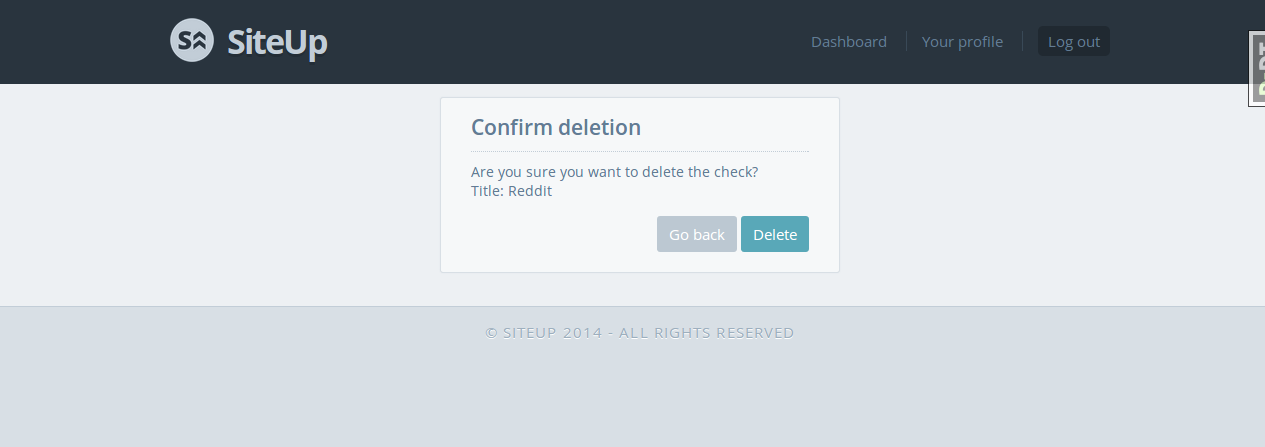
\includegraphics[width=\textwidth]{5_diseno/web-delete}
  \caption{Pantalla genérica de borrado}
  \label{fig:web-delete}
\end{figure}

En la figura~\ref{fig:web-delete} se representa la pantalla de confirmación de
borrado que aparece cuando se intenta borrar un chequeo o un grupo de
chequeos. La pantalla es sencilla: pregunta al usuario si desea realmente borrar
el elemento, ofreciendo dos botones, uno para confirmar el borrado y otro para
cancelar la operación. En ambos casos, tras la interacción el sistema redirige
al usuario al \textit{dashboard}.

\subsection{Pantalla del perfil de usuario}

\begin{figure}[htbp]
  \centering
  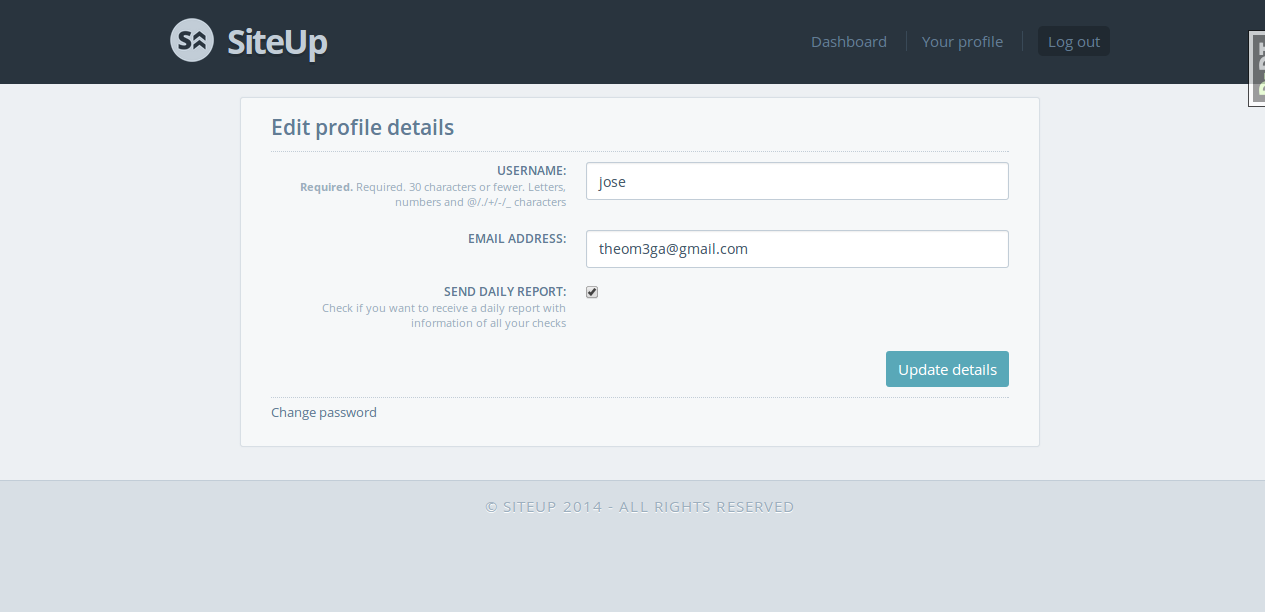
\includegraphics[width=\textwidth]{5_diseno/web-profile}
  \caption{Pantalla del perfil de usuario}
  \label{fig:web-profile}
\end{figure}

En la figura~\ref{fig:web-profile} se muestra la pantalla para editar el perfil
de usuario, a la que se llega pulsando el botón \textit{Your profile} situado en
la barra superior de navegación.

Desde esta pantalla el usuario puede modificar sus datos de usuario: nombre de
usuario, correo electrónico y si desea recibir un reporte diario sobre el estado
de sus chequeos.

También cuenta con la opción de cambiar la contraseña pulsando el botón
\textit{Change password}.


\FloatBarrier
\section{Diseño de la interfaz de usuario de la aplicación móvil}

En esta sección se detallarán las interfaces visuales de la aplicación móvil
para sistemas operativos Android, indicando la navegabilidad e interacción entre
las pantallas.


\subsection{Aspecto desde el lanzador}

\begin{figure}[htbp]
  \centering
  
\includegraphics[width=0.4\textwidth]{5_diseno/android-1}
  \caption{Icono de SiteUp en el lanzador}
  \label{fig:android-launcher}
\end{figure}

La figura~\ref{fig:android-launcher} muestra el aspecto del icono de la aplicación
desde el lanzador de aplicaciones de Android. 

Como se comentó en la sección~\ref{subsec:logotipo}, el logotipo fue diseñado
pensando en su legibilidad en bajas resoluciones, por lo que el icono de la
aplicación es fácilmente identificable desde el lanzador.

Al pulsar el icono de la aplicación, se lanza la pantalla de carga.

\subsection{Pantalla de carga}

\begin{figure}[htbp]
  \centering
  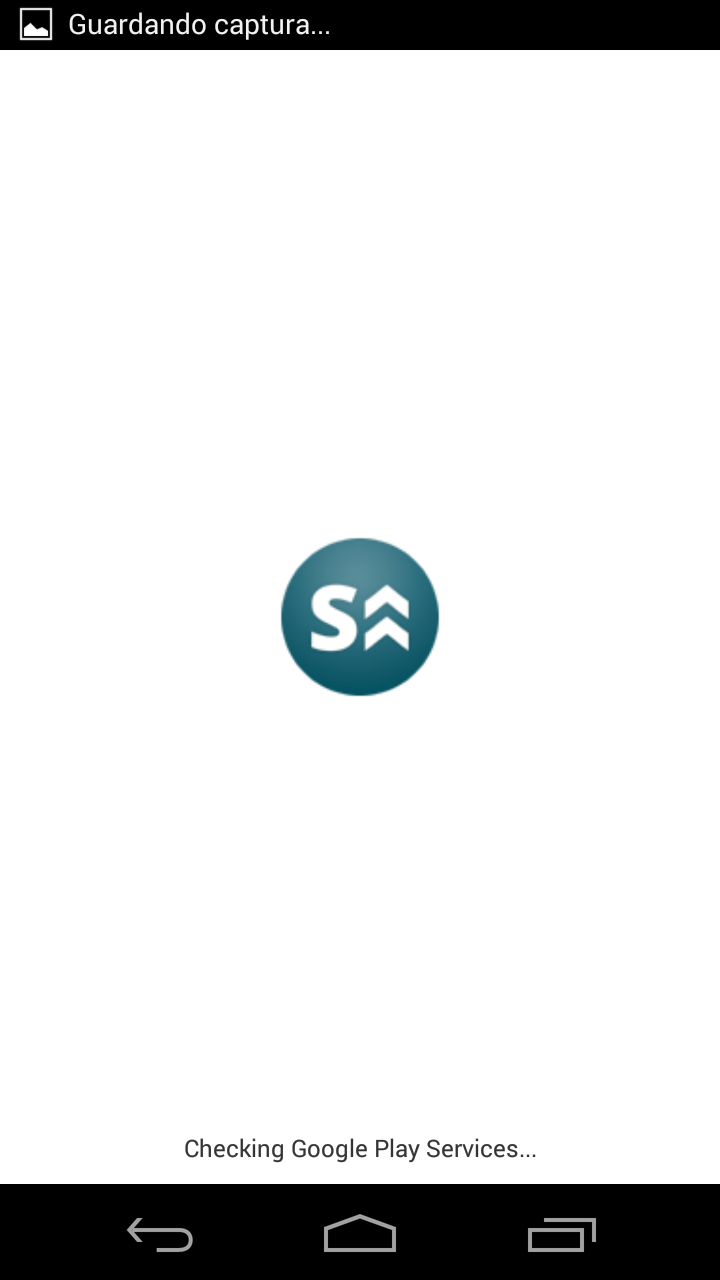
\includegraphics[width=0.4\textwidth]{5_diseno/android-2}
  \caption{Pantalla de carga de la aplicación móvil}
  \label{fig:android-loading}
\end{figure}

En cuanto se pulsa el lanzador aparece la pantalla de carga de la aplicación,
visible en la figura~\ref{fig:android-loading}. Esta pantalla permanece visible
poco tiempo ya que el tiempo de carga es rápido.

Tras el proceso de carga, si la aplicación Android detecta que el usuario ha
iniciado sesión previamente, se carga la pantalla con el listado de chequeos. En
caso de que no haya datos de una sesión anterior, se carga la pantalla de login.

\subsection{Pantalla de inicio de sesión}

\begin{figure}[htbp]
  \centering
  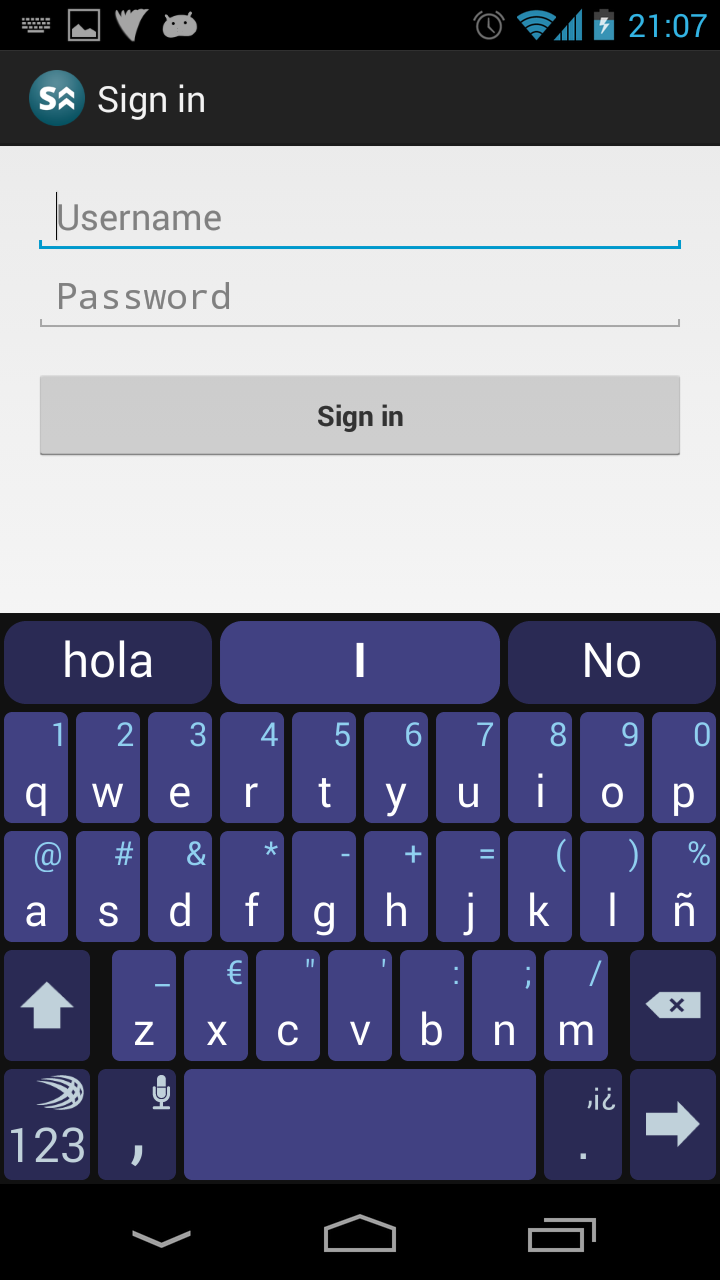
\includegraphics[width=0.4\textwidth]{5_diseno/android-3}
  \caption{Pantalla de inicio de sesión de la aplicación móvil}
  \label{fig:android-login}
\end{figure}

Tras cargar la aplicación, si no se detectan datos de inicio de sesión previos
se muestra la pantalla de inicio de sesión, visible en la
figura~\ref{fig:android-login}, en la que el usuario debe introducir su nombre
de usuario y contraseña para iniciar sesión.

\subsection{Pantalla de listado de chequeos}

\begin{figure}[p]
  \centering
  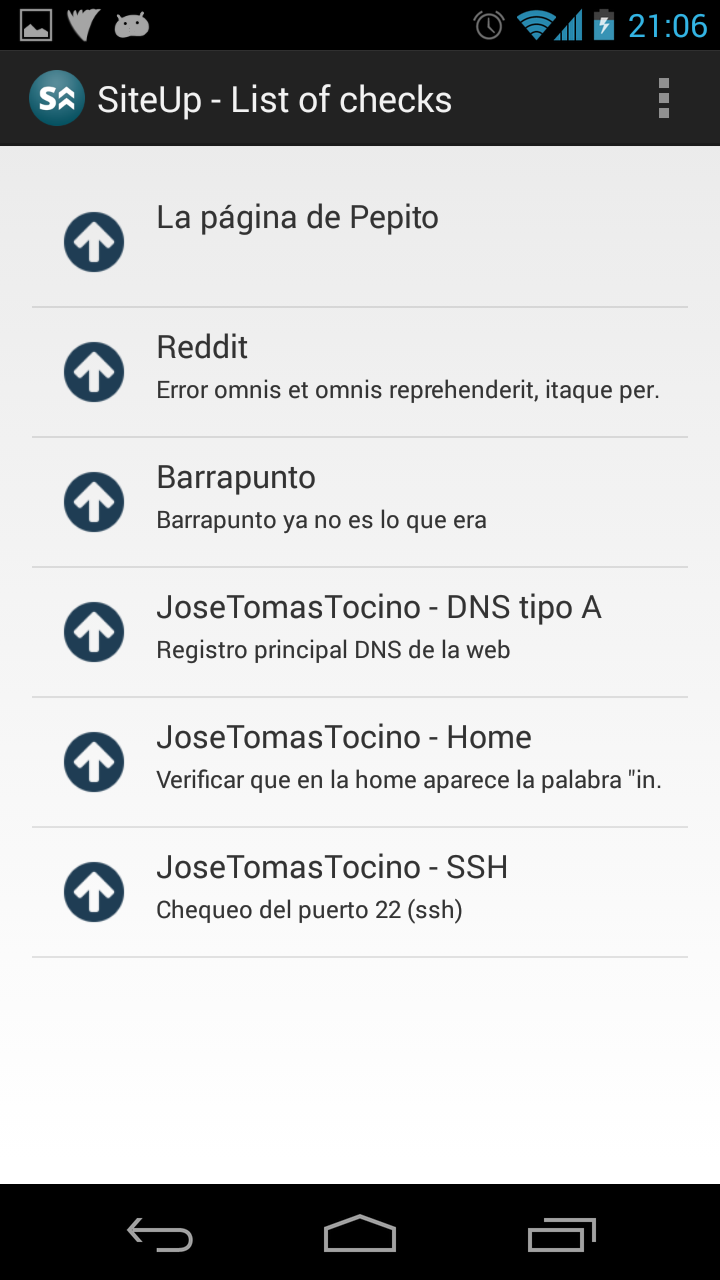
\includegraphics[width=0.4\textwidth]{5_diseno/android-4}
  \caption{Pantalla de chequeos de la aplicación móvil}
  \label{fig:android-dashboard}
\end{figure}

\begin{figure}[p]
  \centering
  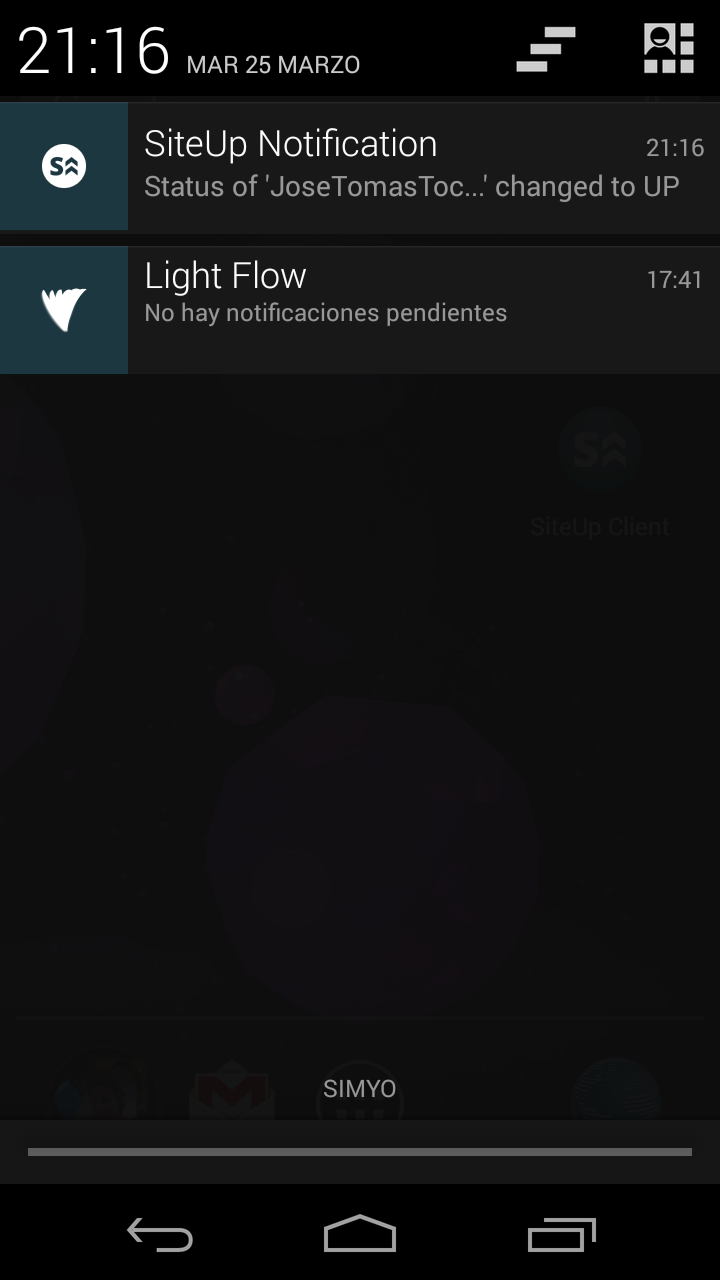
\includegraphics[width=0.4\textwidth]{5_diseno/android-5}
  \caption{Aspecto de las notificaciones}
  \label{fig:android-notification}
\end{figure}

La figura~\ref{fig:android-dashboard} muestra la pantalla con el listado de
chequeos del usuario. Desde aquí es posible cerrar la sesión de usuario, o
pulsar en alguno de los chequeos para ver sus detalles, lo cual abrirá un
navegador y mostrará la plataforma web.

\subsection{Notificación}



La figura~\ref{fig:android-notification} muestra el aspecto que tienen las
notificaciones que la aplicación es capaz de recibir. Desde estas notificaciones
es posible dirigirse a la web para ver los detalles del chequeo involucrado.

%%% Local Variables: 
%%% mode: latex
%%% TeX-master: "../memoria"
%%% End: 


\chapter{Análisis}
\label{chap:analisis}

\section{Metodología}
\textbf{SiteUp} ha seguido una metodología de desarrollo ágil en la que,
mediante fases de desarrollo rápidas y ligeras, se intenta evitar los formales
caminos de las metodologías tradicionales, enfocándose en las personas y
obteniendo así resultados en etapas más tempranas del desarrollo.

En las sucesivas secciones y capítulos se detallará el proceso de análisis y
posteriores fases del proyecto en la última iteración del proyecto. Así se
consigue una documentación más concisa y cercana al producto final.

\section{Modelo conceptual}

De acuerdo a lo reflejado en el apartado~\ref{sec:requisitos-informacion} se
presenta un diagrama en el que se identifican las clases, sus atributos y las
relaciones entre ellas.



% \section{Especificación de requisitos del sistema}

% \subsection{Requisitos de interfaces externas}
% En esta sección describiremos los requisitos que deben cumplir las interfaces
% con el hardware, el software y el usuario.

% En cuanto a la comunicación con el subsistema gráfico y de E/S, utilizaremos la
% biblioteca Gosu~\cite{gosu}, un proyecto de software libre que proporciona un
% framework de desarrollo de videojuegos 2D, multiplataforma y muy sencillo de
% usar. Para el acceso al subsistema de audio, tal y como se ha comentado en la
% sección anterior, optamos por utilizar la API simple de PulseAudio.

% \textbf{oFlute} dispondrá de una resolución fija de 800 por 600 píxeles,
% requisito fácilmente alcanzable en cualquier ordenador actual. Al tratar con un
% público objetivo joven, los gráficos y la interactividad deberán ser sencillos y
% fáciles de interpretar. Así, se ha trabajado en limitar la interacción del
% usuario con la aplicación al uso del ratón y, obviamente, del instrumento
% musical, en este caso la flauta dulce. La navegación resultante de este
% planteamiento queda reflejada en el siguiente diagrama:

% \begin{figure}[h!]
%   \centering
%   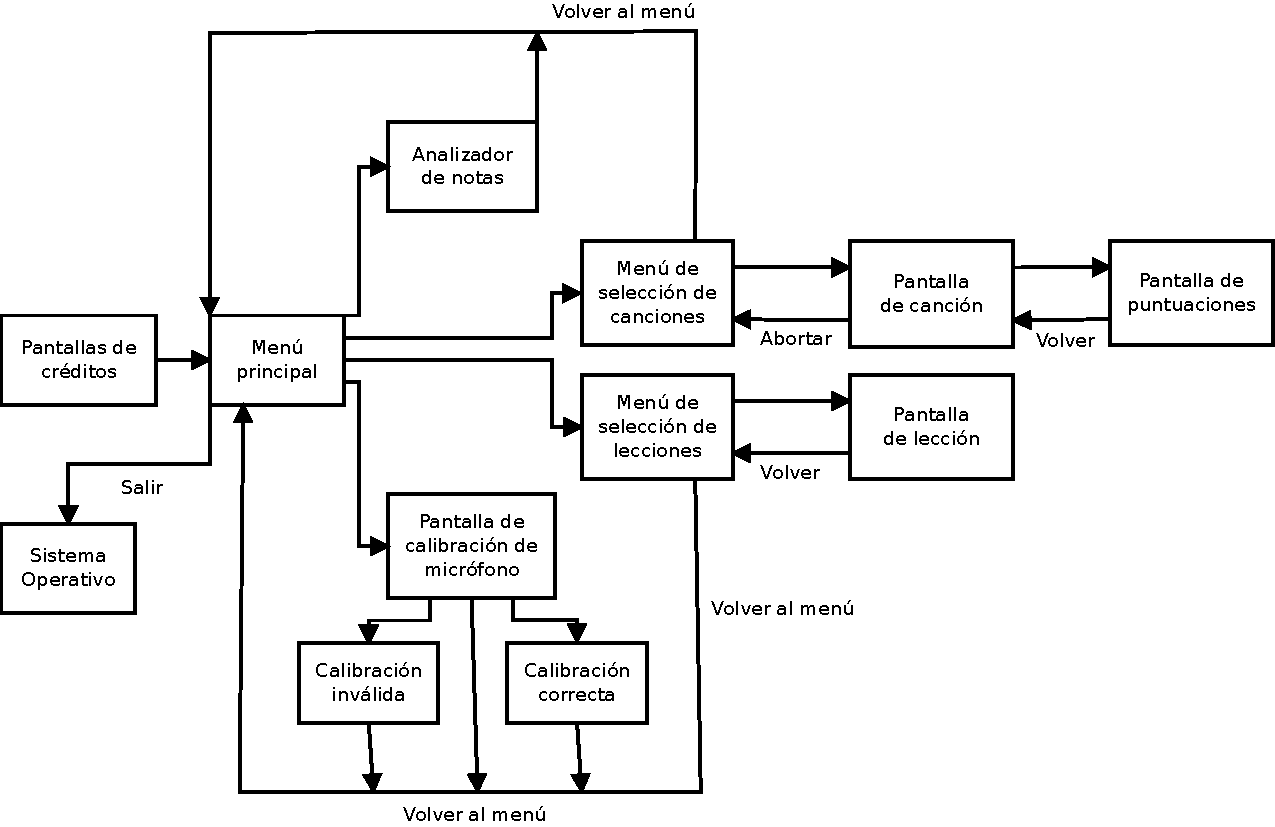
\includegraphics[width=0.9\textwidth]{4_analisis/imagen_diagrama_de_flujo}
%   \caption{Diagrama de flujo de las pantallas de oFlute}
% \end{figure}

% \pagebreak

% Inicialmente, deberán aparecer unas pantallas de crédito con información sobre
% el desarrollador y sobre el propio videojuego. Tras las mismas, que deberá ser
% posible omitir, habrá de aparecer el \textbf{menú principal}, con las cinco
% opciones posibles.

% \begin{figure}[h!]
%   \centering
%   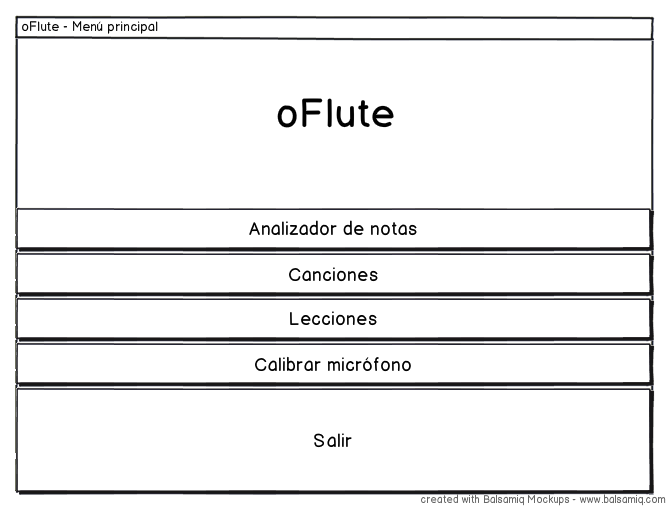
\includegraphics[width=0.6\textwidth]{4_analisis/imagen_mockup_menu_principal}
%   \caption{Maqueta del menú principal}
% \end{figure}

% \pagebreak

% Las opciones que se incluirán son:
% \begin{itemize}
% \item \textbf{Analizador de notas}: comprobar las notas que tocamos sobre un
%   pentagrama.
% \item \textbf{Canciones}: sección principal del juego, en el que aparecerán las
%   canciones a tocar.
% \item \textbf{Lecciones}: sección de lecciones de aprendizaje.
% \item \textbf{Calibrar micrófono}, para ajustarse al nivel de ruido ambiental.
% \item \textbf{Salir} al sistema operativo.
% \end{itemize}

% La siguiente pantalla a modelar será el \textbf{analizador de
%   notas}. Simplemente mostrará el logotipo del videojuego a un lado, y un
% pentagrama al otro, que se actualizará con la nota detectada por el
% micrófono. También contendrá un botón \textit{volver} para ir al menú principal.

% \begin{figure}[h!]
%   \centering
%   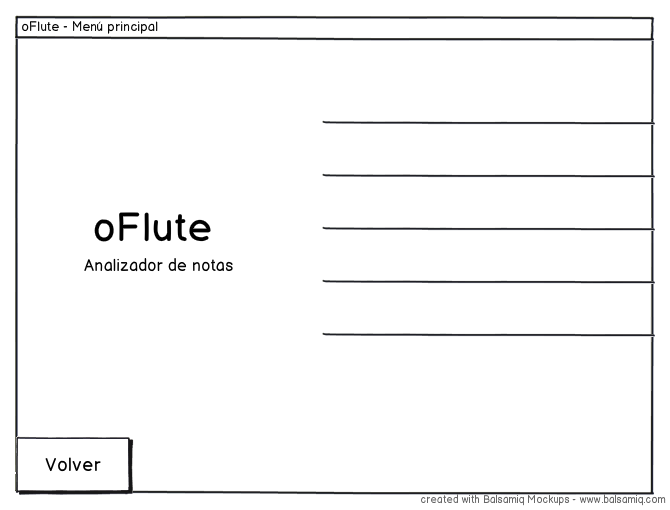
\includegraphics[width=0.6\textwidth]{4_analisis/imagen_mockup_analizador}
%   \caption{Maqueta de la sección \textit{analizador de notas}}
% \end{figure}

% La segunda sección a la que se podrá ir desde el menú principal será la de
% \textbf{canciones}. Inicialmente, la primera pantalla será la de
% \textbf{selección de canción}, que contendrá el logotipo del juego, un botón
% para volver al menú principal, y un menú dinámico de canciones que nos permitirá
% elegir el tema a interpretar.

% \begin{figure}[h!]
%   \centering
%   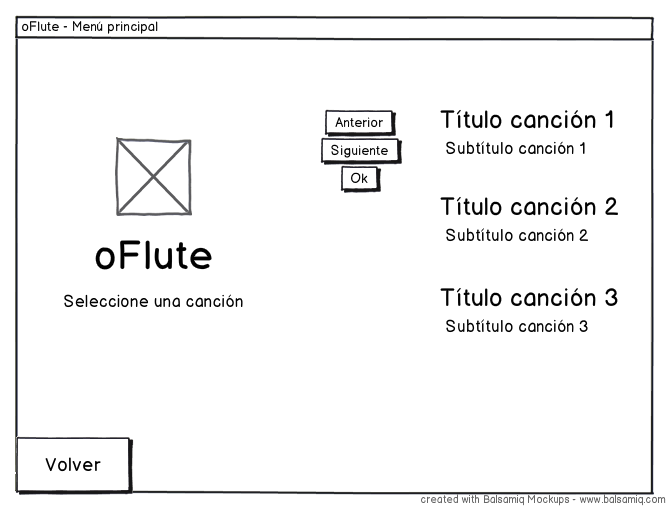
\includegraphics[width=0.6\textwidth]{4_analisis/imagen_mockup_seleccionar_cancion}
%   \caption{Maqueta del menú de selección de canción}
% \end{figure}

% Una vez seleccionada la canción, pasaremos a la zona de \textbf{interpretación
%   de canción}. Contendrá un pentagrama que ocupará todo el ancho de la pantalla,
% con una línea que indicará la zona donde empezar a tocar las notas que
% aparezcan. Además, en la parte superior habrá un indicador con la puntuación
% obtenida y, abajo, una barra de progreso que nos indicará cuánto queda de
% canción.

% \begin{figure}[h!]
%   \centering
%   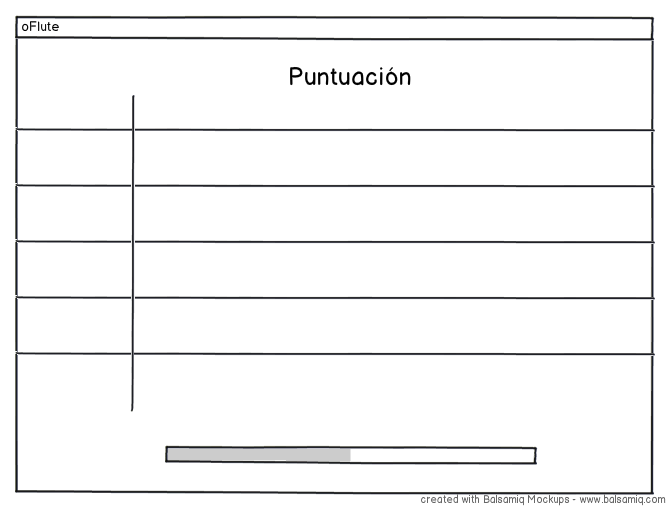
\includegraphics[width=0.6\textwidth]{4_analisis/imagen_mockup_reproducir_cancion}
%   \caption{Maqueta de la pantalla de interpretación de canción}
% \end{figure}

% \pagebreak

% Al completar la interpretación de la canción, aparecerá la \textbf{sección de
%   resultados}. Contendrá el logotipo del juego, el título y subtítulo de la
% canción, y un cuadro con información sobre nuestra interpretación, representada
% en forma de porcentaje de aciertos. Además, en la zona inferior aparecerá un
% mensaje de ánimo dependiendo del resultado obtenido.

% \begin{figure}[h!]
%   \centering
%   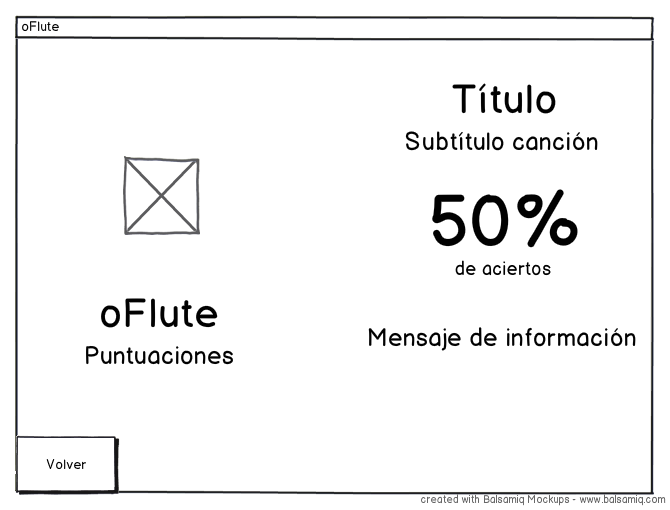
\includegraphics[width=0.6\textwidth]{4_analisis/imagen_mockup_puntuaciones}
%   \caption{Maqueta de la pantalla de puntuaciones}
% \end{figure}

% La pantalla de \textbf{selección de lecciones}, a la que se llega desde el menú
% principal, contendrá el título, una imagen decorativa, y varios botones para
% navegar entre las lecciones cargadas en el sistema. Se mostrará el título y la
% descripción de cada lección, así como un botón para comenzar.

% \begin{figure}[h!]
%   \centering
%   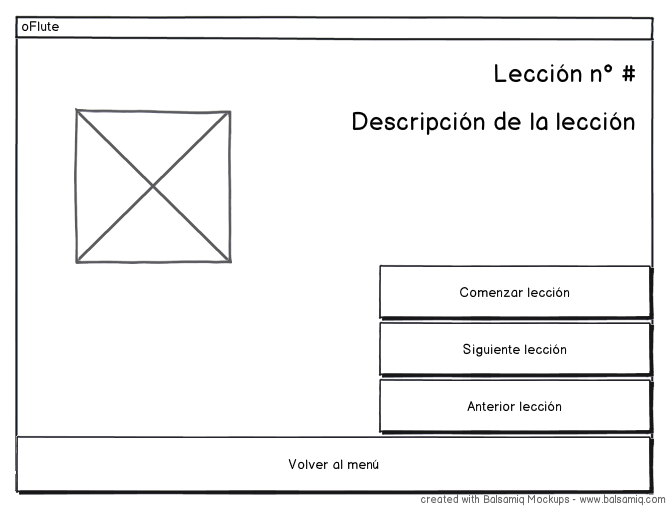
\includegraphics[width=0.6\textwidth]{4_analisis/imagen_mockup_seleccionar_leccion}
%   \caption{Maqueta del menú de selección de lecciones}
% \end{figure}

% Una vez elegida una lección, pasaremos a la pantalla de reproducción de
% lecciones. Dada la naturaleza \textbf{dinámica} de esta sección, cada lección
% podrá tener una apariencia y elementos distintos. El único elemento común entre
% todas las lecciones será el botón de \textbf{volver al menú}.

% \subsection{Requisitos funcionales}

% \textbf{oFlute} se basa en los siguientes requisitos funcionales:
% \begin{itemize}
% \item Poder terminar la aplicación pulsando el botón de cierre en cualquier
%   instante.
% \item Comprobar la correcta interpretación de notas individuales mediante el
%   analizador de notas.
% \item Calibrar el micrófono de forma que el sistema se pueda adaptar al ruido
%   ambiental del entorno.
% \item Navegar por toda la aplicación de forma sencilla utilizando solo el ratón.
% \item Elegir entre varias canciones a interpretar, cada una con su título y
%   subtítulo informativos.
% \item Interpretar las canciones mediante el uso de la flauta, siguiendo el
%   pentagrama en pantalla.
% \item Elegir entre bastantes lecciones informativas, poder ejecutarlas y
%   seguirlas.
% \item Capacidad de añadir nuevas lecciones y canciones de forma sencilla.
% \end{itemize}

% \subsection{Requisitos de rendimiento}

% La aplicación \textbf{oFlute} precisa de unos requisitos bastante básicos,
% que en su mayor parte se reducen a cuatro puntos principales:
% \begin{itemize}
% \item Posesión de una tarjeta de sonido o subsistema de audio similar con un
%   micrófono, para poder captar el sonido de la flauta.
% \item Pantalla con una resolución de, al menos, 800 por 600 píxeles.
% \item Sistema gráfico compatible con OpenGL.
% \item Dispositivo apuntador, como un ratón.
% \end{itemize}

% La práctica totalidad de los ordenadores personales de la actualidad cumplen los
% citados requisitos.

% \subsection{Requisitos del sistema software}
% El sistema de software deberá cumpliar los requisitos siguientes:
% \begin{itemize}
% \item Deberá funcionar en cualquier sistema \textbf{GNU/Linux} con los
%   requisitos anteriormente indicados.
% \item Deberá limitarse el número de dependencias, así como facilitar al máximo
%   la instalación de las que resultasen imprescindibles.
% \item El uso del teclado quedará en segundo plano, haciendo posible utilizar la
%   aplicación completamente con el ratón.
% \item Al tratarse de un público objetivo juvenil, la aplicación deberá ser
%   dinámica, intuitiva y fácil de usar, y la apariencia debe ser agradable.
% \item Se evitará el uso de constantes y recursos dentro del código de la
%   aplicación, utilizando como alternativa ficheros para representar las
%   lecciones y las canciones.
% \end{itemize}

% \section{Modelo de casos de uso}

% A la hora de modelar los casos de uso del sistema, hemos optado por utilizar
% notación \textit{UML}, siguiendo los siguientes pasos:
% \begin{itemize}
% \item Identificación de los usuarios del sistema y sus roles.
% \item Para cada rol, determinar las formas de interactuar con el sistema.
% \item Creación de casos de uso para los objetivos que debe cumplir la aplicación.
% \item Modularización de los casos de usos mediante la implementación de
%   relaciones de inclusión o extensión.
% \end{itemize}

% \subsection{Diagrama de casos de uso}

% \begin{figure}[h!]
%   \centering
%   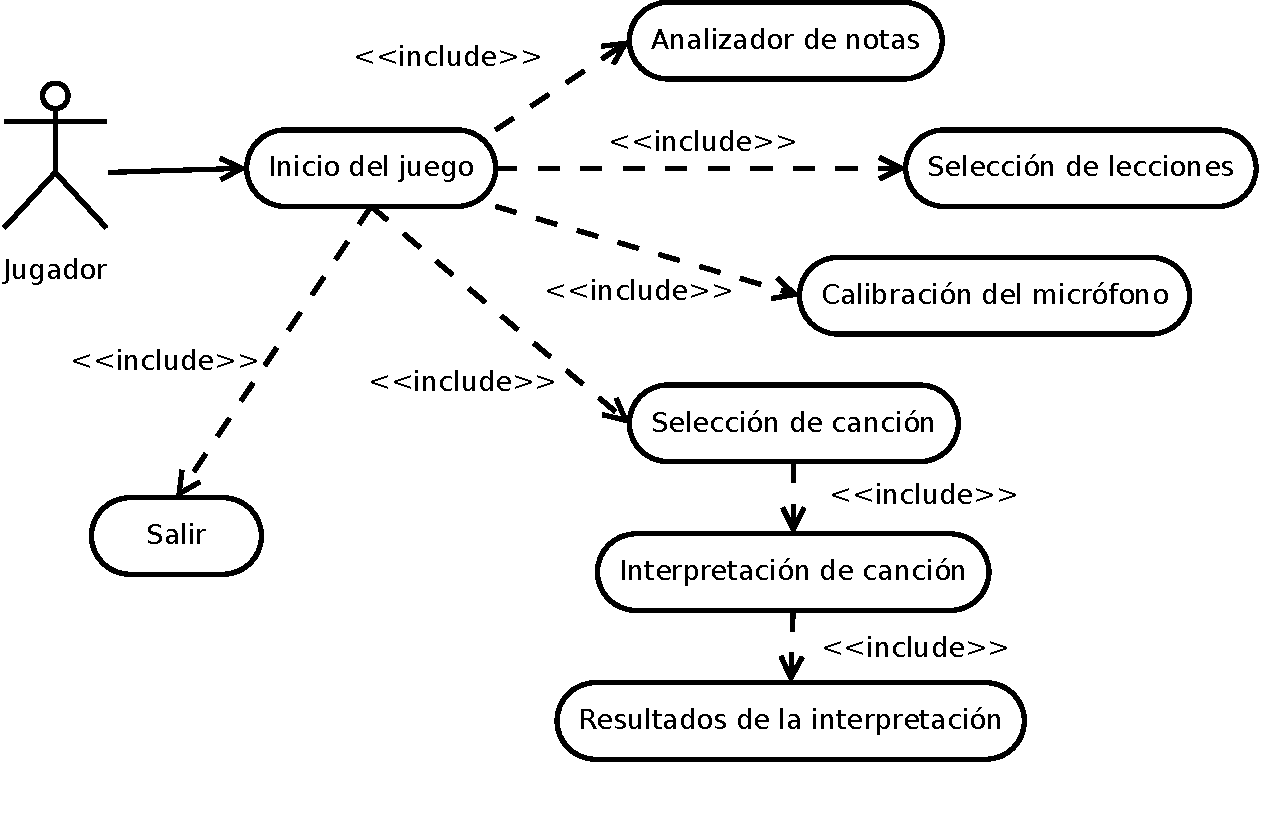
\includegraphics[width=0.81\textwidth]{4_analisis/imagen_diagrama_de_casos_de_uso}
%   \caption{Diagrama de casos de uso}
% \end{figure}


% \subsection{Descripción de los casos de uso}

% \subsubsection{Caso de uso: inicio del juego}
% \begin{description}
% \item [Descripción] Se muestran los créditos del juego, la pantalla de
%   presentación, y finalmente el menú principal, desde donde se accederá al
%   resto de secciones del juego.
% \item [Actores] \jugador.
% \item [Precondiciones] Ninguna.
% \item [Postcondiciones] Ninguna.
% \item [Escenario principal] $\quad$
%   \begin{enumerate}
%   \item El \jugador\ inicia la aplicación.
%   \item El \sistema\ inicializa el subsistema gráfico.
%   \item El \sistema\ muestra la pantalla de créditos y la pantalla de
%     presentación de la aplicación.
%   \item El \sistema\ muestra el menú principal en la pantalla.
%   \item El \jugador\ selecciona la opción \textit{Canciones}.
%   \item El \sistema\ accede a la pantalla de \textit{Selección de canción}.
%   \end{enumerate}
% \item[Extensiones --- flujo alternativo] $\quad$
%   \begin{description}
%   \item [*a] El \jugador\ cierra la ventana.
%     \begin{enumerate}
%     \item El \sistema\ libera los recursos y sale de la aplicación.
%     \end{enumerate}
%   \item [4a] El \jugador\ selecciona la opción \textit{Analizador de Notas}.
%     \begin{enumerate}
%     \item El \sistema\ accede a la pantalla del analizador de notas.
%     \end{enumerate}

%   \item[4b] El \jugador\ selecciona la opción \textit{Lecciones}.
%     \begin{enumerate}
%     \item El \sistema\ accede a la pantalla de \textit{Selección de lecciones}.
%     \end{enumerate}
%   \item[4c] El \jugador\ selecciona la opción \textit{Calibrar micrófono}.
%     \begin{enumerate}
%     \item El \sistema\ accede a la pantalla de calibración de micrófono.
%     \end{enumerate}
%   \item [4d] El \jugador\ selecciona la opción Salir.
%     \begin{enumerate}
%     \item El \sistema\ libera los recursos y sale de la aplicación.\\
%     \end{enumerate}
%   \end{description}  
% \end{description}


% \subsubsection{Caso de uso: selección de canción}

% \begin{description}
% \item [Descripción] Al \jugador\ se le muestra una lista de las canciones
%   detectadas, y éste debe elegir entre ellas la que desea interpretar, o volver
%   al menú princial.
% \item [Actores] \jugador.
% \item [Precondiciones] Ninguna.
% \item [Postcondiciones] Una canción queda seleccionada.
% \item [Escenario principal] $\quad$
%   \begin{enumerate}
%   \item El \jugador\ accede, desde el menú principal, al panel de selección de canciones.
%   \item El \sistema\ busca las canciones dadas de alta en el juego y muestra un menú con las mismas.
%   \item El \jugador\ navega entre las canciones listadas y selecciona una de ellas, pulsando finalmente el botón \textit{Ok}.
%   \item El \sistema\ carga la canción y pasa a la pantalla de interpretación de canciones.
%   \end{enumerate}
% \item[Extensiones --- flujo alternativo] $\quad$
%   \begin{description}
%   \item [*a] El \jugador\ cierra la ventana.
%     \begin{enumerate}
%     \item El \sistema\ libera los recursos y sale de la aplicación.
%     \end{enumerate}
%   \item [3a] El \jugador\ selecciona la opción \textit{Volver}.
%     \begin{enumerate}
%     \item El \sistema\ muestra la animación de cierre y vuelve al menú principal.
%     \end{enumerate}
%   \end{description}  
% \end{description}


% \subsubsection{Caso de uso: interpretación de canción}

% \begin{description}
% \item [Descripción] Tras haber elegido la canción a interpretar, se muestra una
%   partitura con las notas que el \jugador\ deberá tocar para conseguir la puntuación deseada.
% \item [Actores] \jugador.
% \item [Precondiciones] Se ha elegido una canción.
% \item [Postcondiciones] Se completa la interpretación de la canción, obteniendo una calificación
% \item [Escenario principal] $\quad$
%   \begin{enumerate}
%   \item El \sistema\ carga la canción, leyendo las notas, y muestra en pantalla,
%     mediante animaciones, el marcador de puntos y el pentagrama.
%   \item El \sistema\ comienza a mostrar notas en el pentagrama, que van
%     deslizándose hacia el lado izquierdo, en el que se encuentra la aguja de
%     reproducción, e inicia el análisis del sonido.
%   \item El \jugador\, al llegar la nota a la aguja de reproducción, toca la
%     flauta con la altura y la duración correcta, de forma que el micrófono sea
%     capaz de captar el sonido.
%   \item El \sistema\ analiza el sonido que captura el micrófono y detecta la nota que toca el usuario.
%   \item El \sistema\ determina que la nota es la correcta y suma los puntos correspondientes.
%   \item Mientras existan más notas, se vuelve al punto 2.
%   \item El \sistema\ determina que no hay más notas que mostrar, e inicia las
%     animaciones para ocultar los elementos en pantalla.
%   \item El \sistema\ pasa a la sección de \textit{Resultados de la interpretación}.
%   \end{enumerate}
% \item[Extensiones --- flujo alternativo] $\quad$
%   \begin{description}

%   \item [*a] El \jugador\ cierra la ventana.
%     \begin{enumerate}
%     \item El \sistema\ libera los recursos y sale de la aplicación.
%     \end{enumerate}

%   \item[*b] El \jugador\ pulsa la tecla \texttt{escape}.
%     \begin{enumerate}
%     \item El \sistema\ vuelve a la pantalla de \textit{selección de canción}.
%     \end{enumerate}

%   \item [3a] El \jugador\ toca el instrumento con intensidad insuficiente o nula
%     y el sonido no llega al sistema.
%     \begin{enumerate}
%     \item El \sistema\ representa esta inconsistencia como un silencio.
%     \end{enumerate}

%   \item [4a] El \sistema\ no es capaz de determinar fehacientemente la nota que
%     toca el usuario.
%     \begin{enumerate}
%     \item El \sistema\ representa esta inconsistencia como un silencio.
%     \end{enumerate}

%   \item[5a] El \sistema\ determina que la nota tocada por el usuario no es la
%     que corresponde a la partitura.
%     \begin{enumerate}
%     \item El \sistema\ ignora esta situación y no suma los puntos al marcador.
%     \end{enumerate}

%   \end{description}  
% \end{description}

% \subsubsection{Caso de uso: resultados de la interpretación}

% \begin{description}
% \item [Descripción] Después de interpretar las notas de la partitura, se
%   muestran los datos obtenidos del análisis de las notas tocadas por el \jugador.
% \item [Actores] \jugador.
% \item [Precondiciones] Se ha elegido e interpretado una canción.
% \item [Postcondiciones] Se completa la partida actual.
% \item [Escenario principal] $\quad$
%   \begin{enumerate}
%   \item El \sistema\ compara la puntuación conseguida con la máxima puntuación
%     obtenible, y genera un porcentaje de aciertos.
%   \item El \sistema\ muestra, mediante animaciones, un mensaje con información
%     sobre la canción y sobre la interpretación del \jugador\, representada
%     mediante un porcentaje de aciertos.
%   \item El \sistema\ muestra un mensaje variable en función del número de
%     aciertos conseguido.
%   \item El \jugador\ revisa su puntuación y pulsa el botón \textit{volver} para
%     ir de vuelta al menú de \textit{selección de canción}.
%   \end{enumerate}
% \item[Extensiones --- flujo alternativo] $\quad$
%   \begin{description}

%   \item [*a] El \jugador\ cierra la ventana.
%     \begin{enumerate}
%     \item El \sistema\ libera los recursos y sale de la aplicación.
%     \end{enumerate}

%   \item[4a] El \jugador\ pulsa la tecla \texttt{escape}.
%     \begin{enumerate}
%     \item El \sistema\ vuelve a la pantalla de \textit{selección de canción}.
%     \end{enumerate}

%   \end{description}  
% \end{description}


% \subsubsection{Caso de uso: analizador de notas}

% \begin{description}
% \item [Descripción] El \jugador\ elige la opción \textit{analizador de notas} en
%   el menú principal y es llevado a esta sección, en la que el sistema
%   representará gráficamente la nota que esté tocando con la flauta en cada
%   instante, sin otra interacción
% \item [Actores] \jugador.
% \item [Precondiciones] Ninguna.
% \item [Postcondiciones] Ninguna
% \item [Escenario principal] $\quad$
%   \begin{enumerate}
%   \item El \jugador\ accede, desde el menú principal, al panel del analizador de notas.
%   \item El \sistema\ muestra, mediante animaciones, la pantalla de la sección,
%     representada mediante una fracción de partitura en la que se representará la
%     nota que esté tocando el \jugador\ en cada momento.
%   \item El \sistema\ inicia el análisis del sonido.
%   \item El \jugador\ toca la nota que desee con su flauta, de forma que el
%     micrófono sea capaz de captar el sonido.
%   \item El \sistema\ analiza el sonido que captura el micrófono y detecta la
%     nota que toca el usuario.
%   \item El \sistema\ muestra en pantalla la nota, sobre la partitura,
%     correspondiente a lo que ha tocado el usuario.
%   \item Se repite el flujo desde el punto 4, mientras el \jugador\ no pulse en
%     el botón volver.
%   \item El \jugador\ pulsa en el botón \textit{volver}.
%   \item El \sistema\ inicia las animaciones para ocultar los elementos en pantalla.
%   \item El \sistema\ vuelve al menú principal.
%   \end{enumerate}
% \item[Extensiones --- flujo alternativo] $\quad$
%   \begin{description}

%   \item [*a] El \jugador\ cierra la ventana.
%     \begin{enumerate}
%     \item El \sistema\ libera los recursos y sale de la aplicación.
%     \end{enumerate}

%   \item[*b] El \jugador\ pulsa la tecla \texttt{escape}.
%     \begin{enumerate}
%     \item El \sistema\ vuelve al menú principal.
%     \end{enumerate}

%   \item [4a] El \jugador\ toca el instrumento con intensidad insuficiente o nula
%     y el sonido no llega al sistema.
%     \begin{enumerate}
%     \item El \sistema\ representa esta inconsistencia como un silencio.
%     \end{enumerate}

%   \item [5a] El \sistema\ no es capaz de determinar fehacientemente la nota que
%     toca el usuario.
%     \begin{enumerate}
%     \item El \sistema\ representa esta inconsistencia como un silencio.
%     \end{enumerate}
%   \end{description}  
% \end{description}

% \subsubsection{Caso de uso: calibración de micrófono}
% \begin{description}
% \item [Descripción] El \jugador\ elige la opción \textit{calibrar micrófono} en
%   el menú principal y es llevado a esta sección, en la que el \sistema\ calibrará
%   el micrófono de forma que sea posible aislar el sonido de la flauta del ruido
%   ambiental.
% \item [Actores] \jugador.
% \item [Precondiciones] Ninguna.
% \item [Postcondiciones] El \sistema\ obtiene un valor umbral con el que
%   discernir entre el sonido del instrumento y el ruido ambiente.
% \item [Escenario principal] $\quad$
%   \begin{enumerate}
%   \item El \jugador\ accede, desde el menú principal, al panel de calibración del micrófono.
%   \item El \sistema\ muestra la sección, indicando con un mensaje que el usuario
%     debe pulsar la tecla \texttt{escape} para iniciar la calibración.
%   \item El \jugador\ pulsa la tecla \texttt{escape} y se mantiene en silencio.
%   \item El \sistema\ inicia el análisis del sonido, guardando durante dos
%     segundos los valores de ruido que lee del micrófono.
%   \item El \sistema\ calcula, a partir de los valores leídos, el umbral de
%     ruido, y muestra un mensaje informando del final del proceso.
%   \item El \jugador\ pulsa la tecla \texttt{escape} y el \sistema\ vuelve al
%     menú principal.
%   \end{enumerate}
% \item[Extensiones --- flujo alternativo] $\quad$
%   \begin{description}

%   \item [*a] El \jugador\ cierra la ventana.
%     \begin{enumerate}
%     \item El \sistema\ libera los recursos y sale de la aplicación.
%     \end{enumerate}

%   \item[*b] El \jugador\ pulsa la tecla \texttt{escape}.
%     \begin{enumerate}
%     \item El \sistema\ cancela la calibración y vuelve al menú principal.
%     \end{enumerate}

%   \item [5a] El \sistema\ encuentra valores inválidos al leer el ruido
%     ambiental.
%     \begin{enumerate}
%     \item El \sistema\ informa al usuario del fallo del proceso de calibración.
%     \item El \jugador\ pulsa la tecla \texttt{escape} y el \sistema\ vuelve al
%       menú principal.
%     \end{enumerate}
%   \end{description}  
% \end{description}

% \subsubsection{Caso de uso: selección de lecciones}
% \begin{description}
% \item [Descripción] El \jugador\ elige la opción \textit{lecciones} en el menú
%   principal y es llevado a esta sección, en la que el \sistema\ mostrará una
%   lista de lecciones cargadas, entre las que el usuario deberá elegir.
% \item [Actores] \jugador.
% \item [Precondiciones] Ninguna.
% \item [Postcondiciones] Se ha elegido una lección
% \item [Escenario principal] $\quad$
%   \begin{enumerate}
%   \item El \jugador\ accede, desde el menú principal, al panel de selección de lecciones.
%   \item El \sistema\ carga la lista de secciones y muestra, mediante
%     animaciones, el panel, preseleccionando por defecto la primera lección.
%   \item El \jugador\ utiliza los botones de la sección para elegir una de las
%     lecciones, y activarla pulsando \textit{comenzar lección}.
%   \item El \sistema\ oculta de forma animada el panel de selección de lecciones.
%   \item El \sistema\ lee el fichero \texttt{xml} asociado a la lección indicada,
%     cargando los elementos que la componen y las animaciones que se ejecutarán.
%   \item El \sistema\ ejecuta las animaciones correspondientes a los elementos
%     multimedia de la lección.
%   \end{enumerate}
% \item[Extensiones --- flujo alternativo] $\quad$
%   \begin{description}

%   \item [*a] El \jugador\ cierra la ventana.
%     \begin{enumerate}
%     \item El \sistema\ libera los recursos y sale de la aplicación.
%     \end{enumerate}

%   \item[2a] El \sistema\ detecta que una de las lecciones leídas no está
%     correctamente construída.
%     \begin{enumerate}
%     \item El \sistema\ informa del error en el \textit{log} del programa y omite
%       la carga de esa lección.
%     \end{enumerate}

%   \item[3a] El \jugador\ pulsa la tecla \texttt{escape}.
%     \begin{enumerate}
%     \item El \sistema\ vuelve al menú principal.
%     \end{enumerate}

%   \item[6a] El \jugador\ pulsa la tecla \texttt{escape}.
%     \begin{enumerate}
%     \item El \sistema\ vuelve al menú de selección de lecciones.
%     \end{enumerate}

%   \end{description}  
% \end{description}

% \section{Modelo conceptual de datos}

% El modelo conceptual de datos representa, de forma esquemática, las clases que
% modelan el sistema y las relaciones que existen entre ellas, además de una
% pequeña introducción a su utilidad. 

% \begin{description}
% \item[Juego] Clase de control general. Gestiona el flujo de ejecución principal,
%   así como de la gestión de estados, que permite pasar de una sección a otra del
%   juego.
% \item[Estado] Clase base para los diferentes estados del juego. Las clases
%   correspondientes a las secciones se basarán en esta clase para interactuar con
%   el gestor de estados y poder pasar de una parte del juego a otra.
% \item[EstadoMenú] Representa el estado de juego para el menú principal, desde el
%   que se accede al resto de opciones del juego. 
% \item[EstadoAnalizador] Representa el estado del analizador básico de
%   notas. Contendrá los elementos necesarios para iniciar el análisis del audio,
%   así como los elementos de la interfaz.
% \item[EstadoCalibrarMicro] Representa el estado en el que se calibra el
%   micrófono. Al igual que la clase \textit{EstadoAnalizador}, deberá ser capaz
%   de acceder al sistema de audio para poder leer el volumen ambiente y así
%   calibrar el micrófono.
% \item[EstadoImagenFija] Modela una imagen fija a modo de pantalla de créditos,
%   de forma que sea sencillo añadir imágenes al inicio del juego, como firmas de
%   desarrolladores, logotipos de patrocinadores, etcétera.
% \item[EstadoMenúCanciones] Comprende el menú de selección de canciones, que se
%   encargará de leer los ficheros de canciones disponibles. Además, también se
%   encargará de lanzar las canciones en forma de estados secundarios.
% \item[EstadoCanción] Corresponde a la canción que se va a interpretar, lanzada desde
%   el estado \textit{EstadoMenuCanciones}.
% \item[EstadoMenúLecciones] Corresponde al menú de elección de lecciones, que
%   leerá y listará los ficheros de lección disponibles, y se encargará de lanzar
%   la lección elegida.
% \item[EstadoLección] Corresponde a la canción elegida desde el menú
%   \textit{EstadoMenúLecciones}.
% \item[Analizador] Controla la gestión del subsistema de audio y el análisis de
%   la entrada. Deberá proporcionar información sobre el volumen de la entrada
%   (para la calibración del micrófono) así como de la nota detectada en cada
%   instante.
% \item[Animación] Se encargará de facilitar la creación de animaciones en forma
%   de interpolación de valores, válidas para cambios de posición, opacidad,
%   etcétera.
% \item[Elemento] Esta clase de ayuda facilitará la carga y dibujado de elementos
%   para la interfaz, además de servir de capa de abstracción para las
%   animaciones.
% \item[ElementoImagen] Especialización de la clase \textit{Elemento} para
%   imágenes.
% \item[ElementoTexto] Especialización de la clase \textit{Elemento} para textos.
% \item[ElementoCombinado] Especialización de la clase \textit{Elemento} que
%   combina imagen y texto, a usar en casos como los botones del menú.
% \item[SistemaPartículas] Representa un sistema de partículas simple, para
%   generar efectos de destellos y fuegos artificiales.
% \item[Nota] Simboliza cada una de las notas cargadas que componen una canción.
% \end{description}

% \begin{figure}[htp!]
%   \centering
%   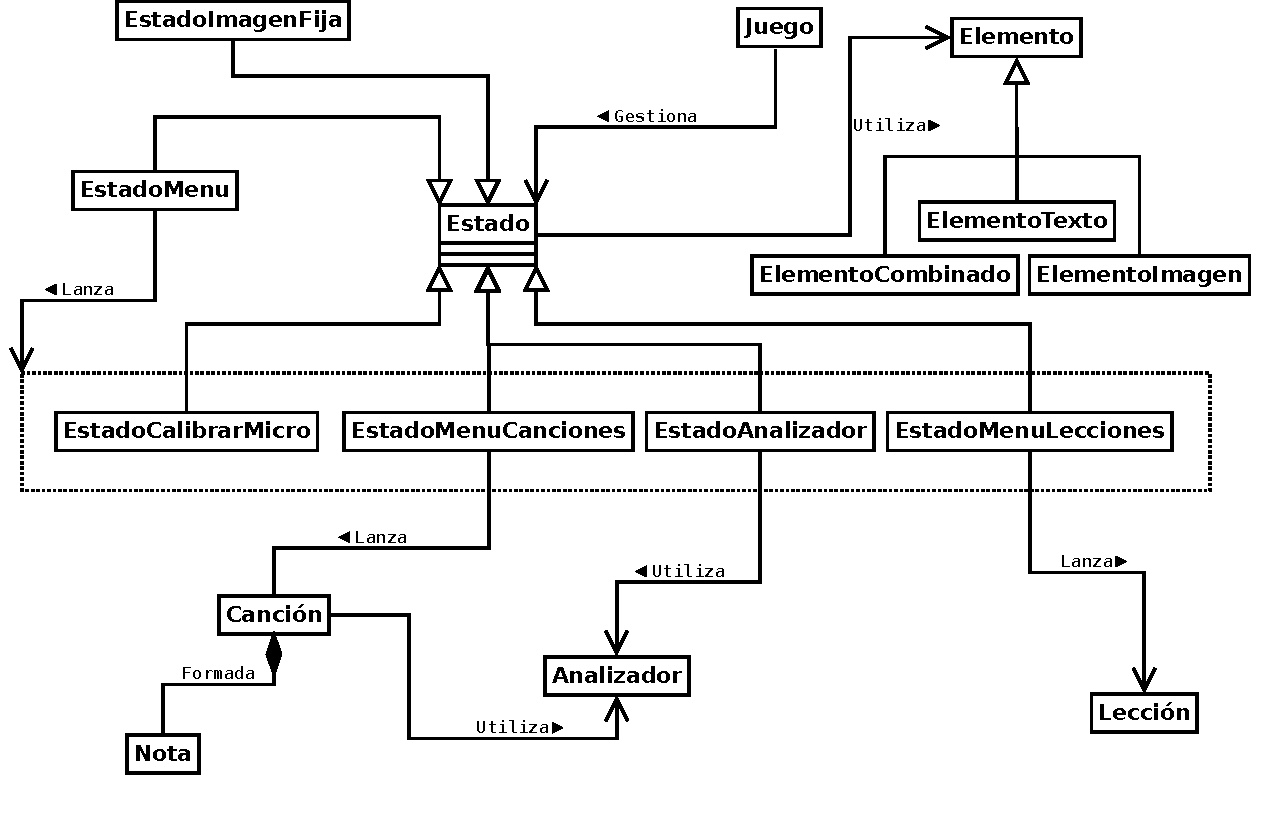
\includegraphics[angle=90]{4_analisis/imagen_diagrama_clases_conceptuales}
%   \caption{Diagrama de clases conceptuales}
% \end{figure}

% \pagebreak

%
\section{Modelo de comportamiento del sistema}
En esta sección vamos a especificar cómo se comporta el sistema en forma de dos
elementos fundamentales.
\begin{itemize}
\item En primer lugar, los \textbf{diagramas de secuencia} mostrarán el flujo de
  eventos entre los actores que participan en la aplicación.
\item En segundo lugar, los \textbf{contratos de las operaciones} detallarán las
  condiciones y efectos que tendrán lugar al ejecutarse las operaciones en el
  sistema.
\end{itemize}

\begin{nota}
  No se han reflejado, por triviales, los escenarios alternativos en los que el
  usuario cierra la ventana, correspondientes a los flujos \textit{*a} definidos
  en la sección anterior.
\end{nota}

\subsection{Caso de uso: inicio del juego}

\subsubsection{Escenario principal}

\begin{figure}[h!]
  \centering
  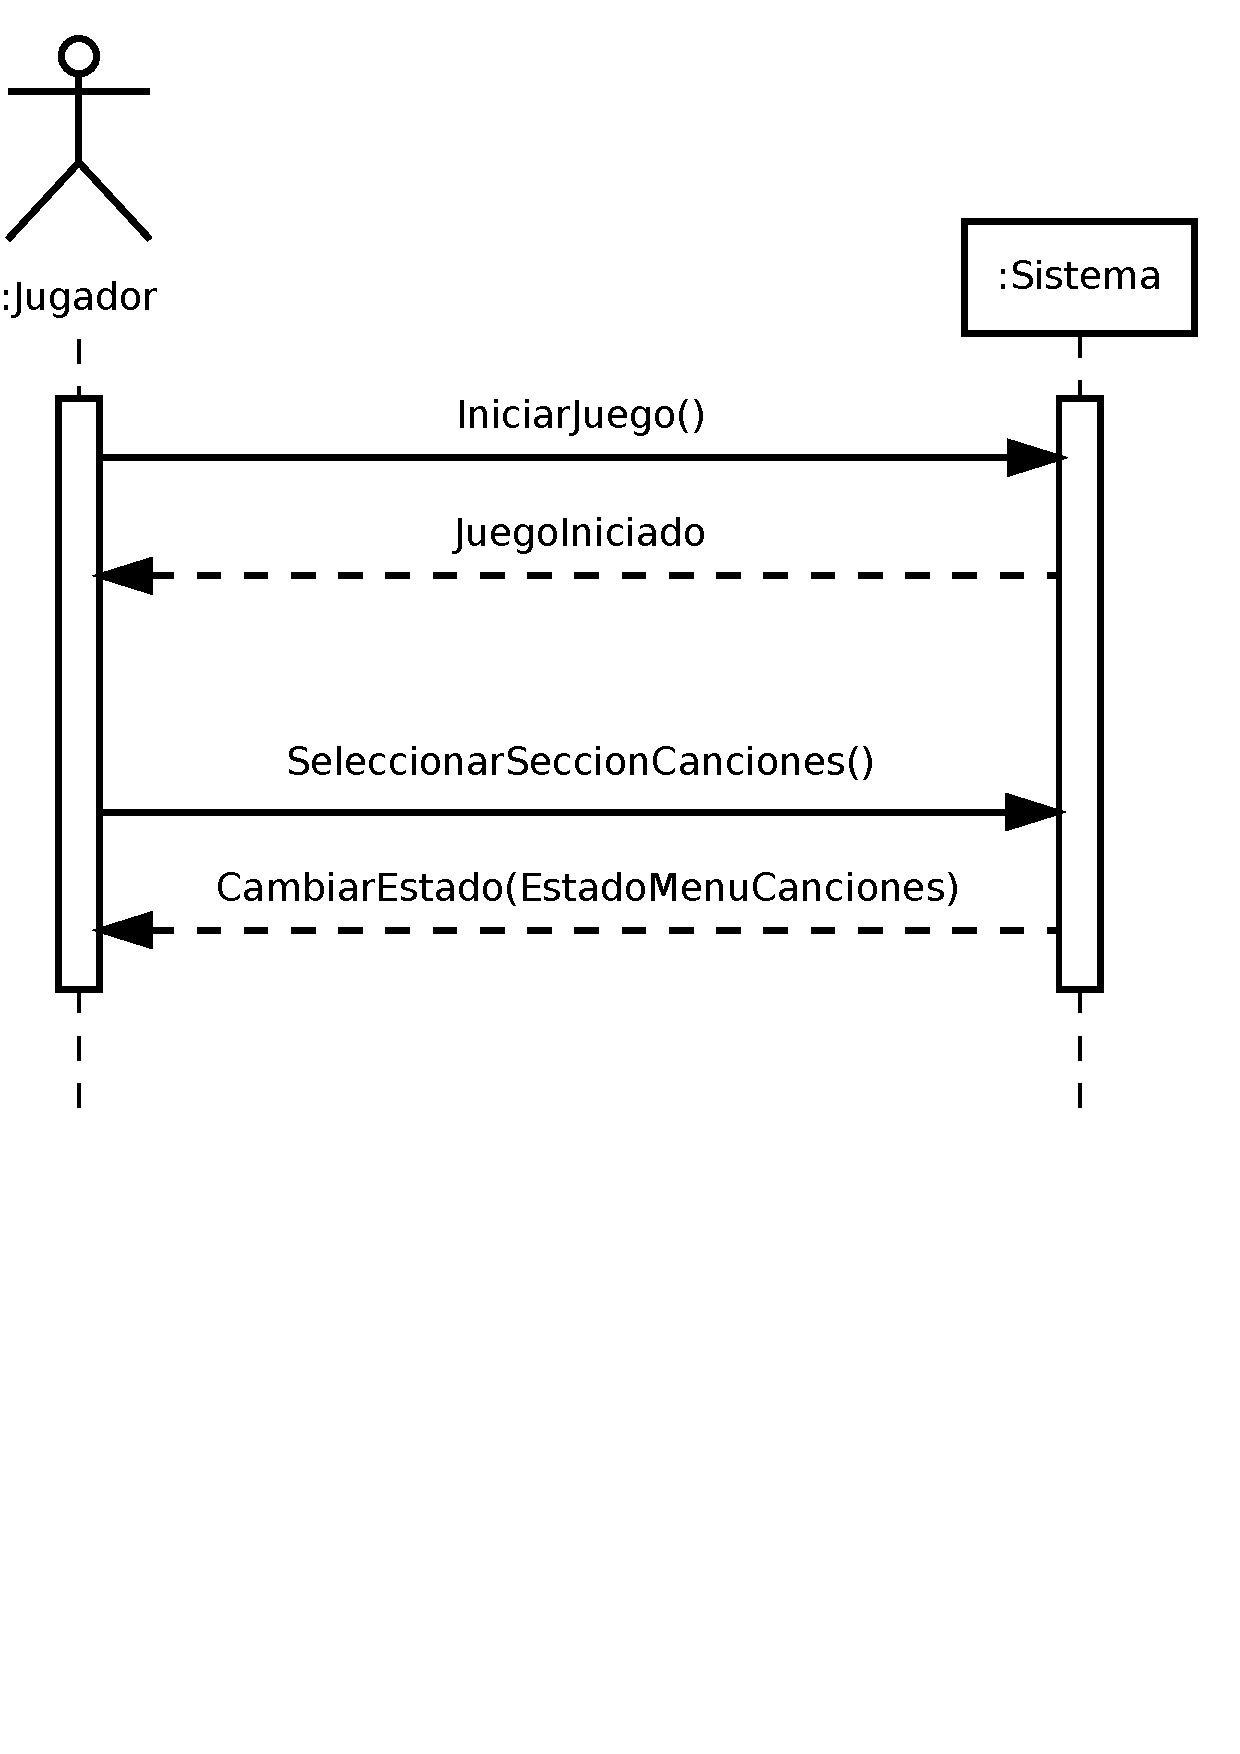
\includegraphics[trim=0cm 12cm 0cm 0cm, clip=true, width=0.5\textwidth]{4_analisis/diagsec_caso1_esc1}
  \caption{Diagrama de secuencia, incio del juego, escenario principal}
\end{figure}

\begin{description}
\item[Operación] IniciarJuego()
\item[Actores] \jugador\, \sistema\
\item[Responsabilidades] Cargar y lanzar la aplicación, mostrar los títulos de
  crédito y el menú principal.
\item[Precondiciones] Ninguna.
\item[Postcondiciones] $\quad$

  \begin{itemize}
  \item Se crea una instancia de la clase \textit{Juego}, que gestiona la
    creación y destrucción de los estados.
  \item Se crean y posteriormente destruyen dos estados
    \textit{EstadoImagenFija} para mostrar los títulos de crédito.
  \item Se crea y permanece un estado \textit{EstadoMenú}, que representa el
    menú principal de la aplicación.
  \end{itemize}

\end{description}

\begin{description}
\item[Operación] SeleccionarSeccionCanciones()
\item[Actores] \jugador\, \sistema\
\item[Responsabilidades] Esconder el menú principal y cargar el menú de
  selección de canciones.
\item[Precondiciones] $\quad$

  \begin{itemize}
  \item El estado actual es una instancia de \textit{EstadoMenú}.
  \end{itemize}

\item[Postcondiciones] Se destruye el estado \textit{EstadoMenú} y se carga
  \textit{EstadoMenúCanciones}.
\end{description}

\subsubsection{Escenario alternativo 4a}
\begin{figure}[h!]
  \centering
  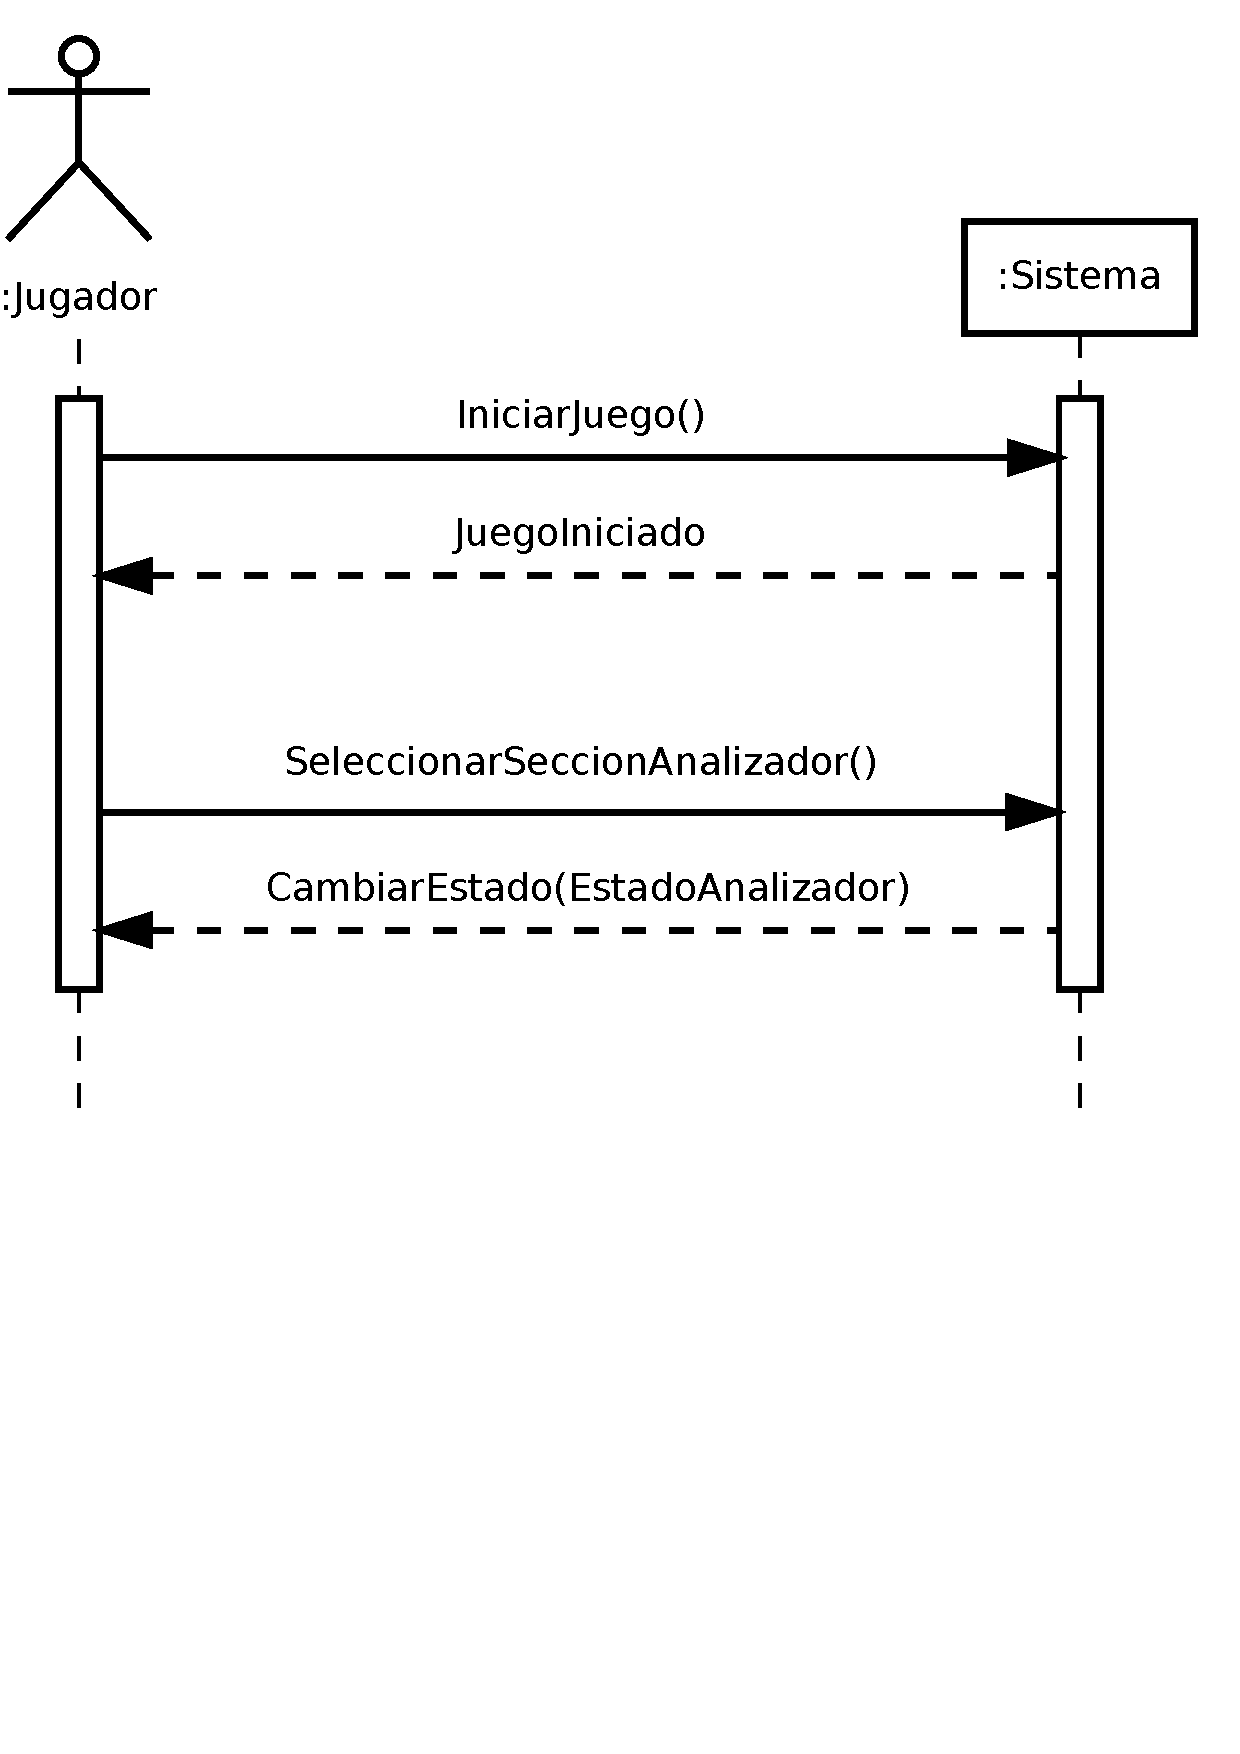
\includegraphics[trim=0cm 12cm 0cm 0cm, clip=true, width=0.5\textwidth]{4_analisis/diagsec_caso1_esc2}
  \caption{Diagrama de secuencia, incio del juego, escenario alternativo 4a}
\end{figure}

\begin{description}
\item[Operación] SeleccionarSeccionAnalizador()
\item[Actores] \jugador\, \sistema\
\item[Responsabilidades] Esconder el menú principal y cargar la sección de
  análisis de notas.
\item[Precondiciones] $\quad$
  \begin{itemize}
  \item El estado actual es una instancia de \textit{EstadoMenú}.
  \end{itemize}
\item[Postcondiciones] Se destruye el estado \textit{EstadoMenú} y se carga
  \textit{EstadoAnalizador}.
\end{description}

\subsubsection{Escenario alternativo 4b}
\begin{figure}[h!]
  \centering
  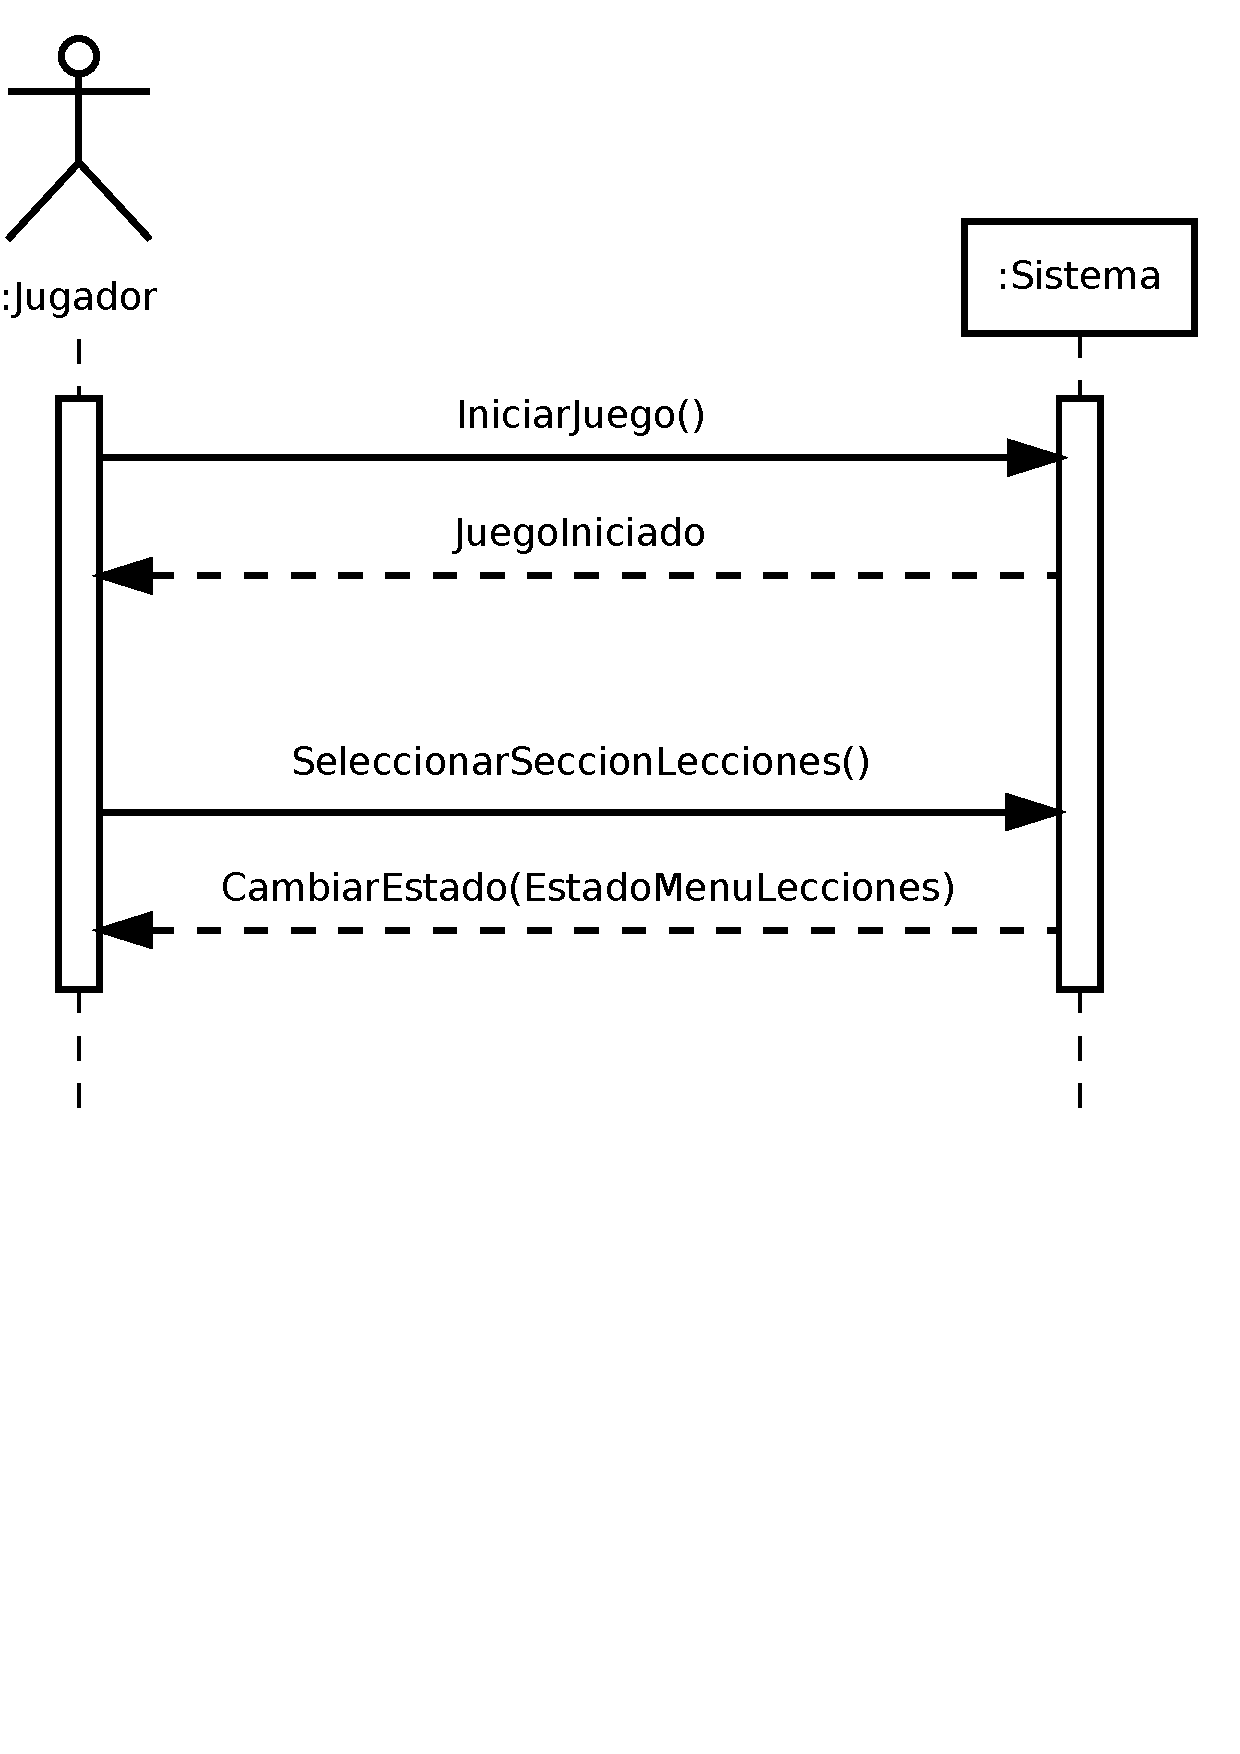
\includegraphics[trim=0cm 12cm 0cm 0cm, clip=true, width=0.5\textwidth]{4_analisis/diagsec_caso1_esc3}
  \caption{Diagrama de secuencia, incio del juego, escenario alternativo 4b}
\end{figure}

\begin{description}
\item[Operación] SeleccionarSeccionLecciones()
\item[Actores] \jugador\, \sistema\
\item[Responsabilidades] Esconder el menú principal y cargar la menú de
  selección de lecciones.
\item[Precondiciones] $\quad$
  \begin{itemize}
  \item El estado actual es una instancia de \textit{EstadoMenú}.
  \end{itemize}
\item[Postcondiciones] Se destruye el estado \textit{EstadoMenú} y se carga
  \textit{EstadoMenúLecciones}.
\end{description}

\subsubsection{Escenario alternativo 4c}
\begin{figure}[h!]
  \centering
  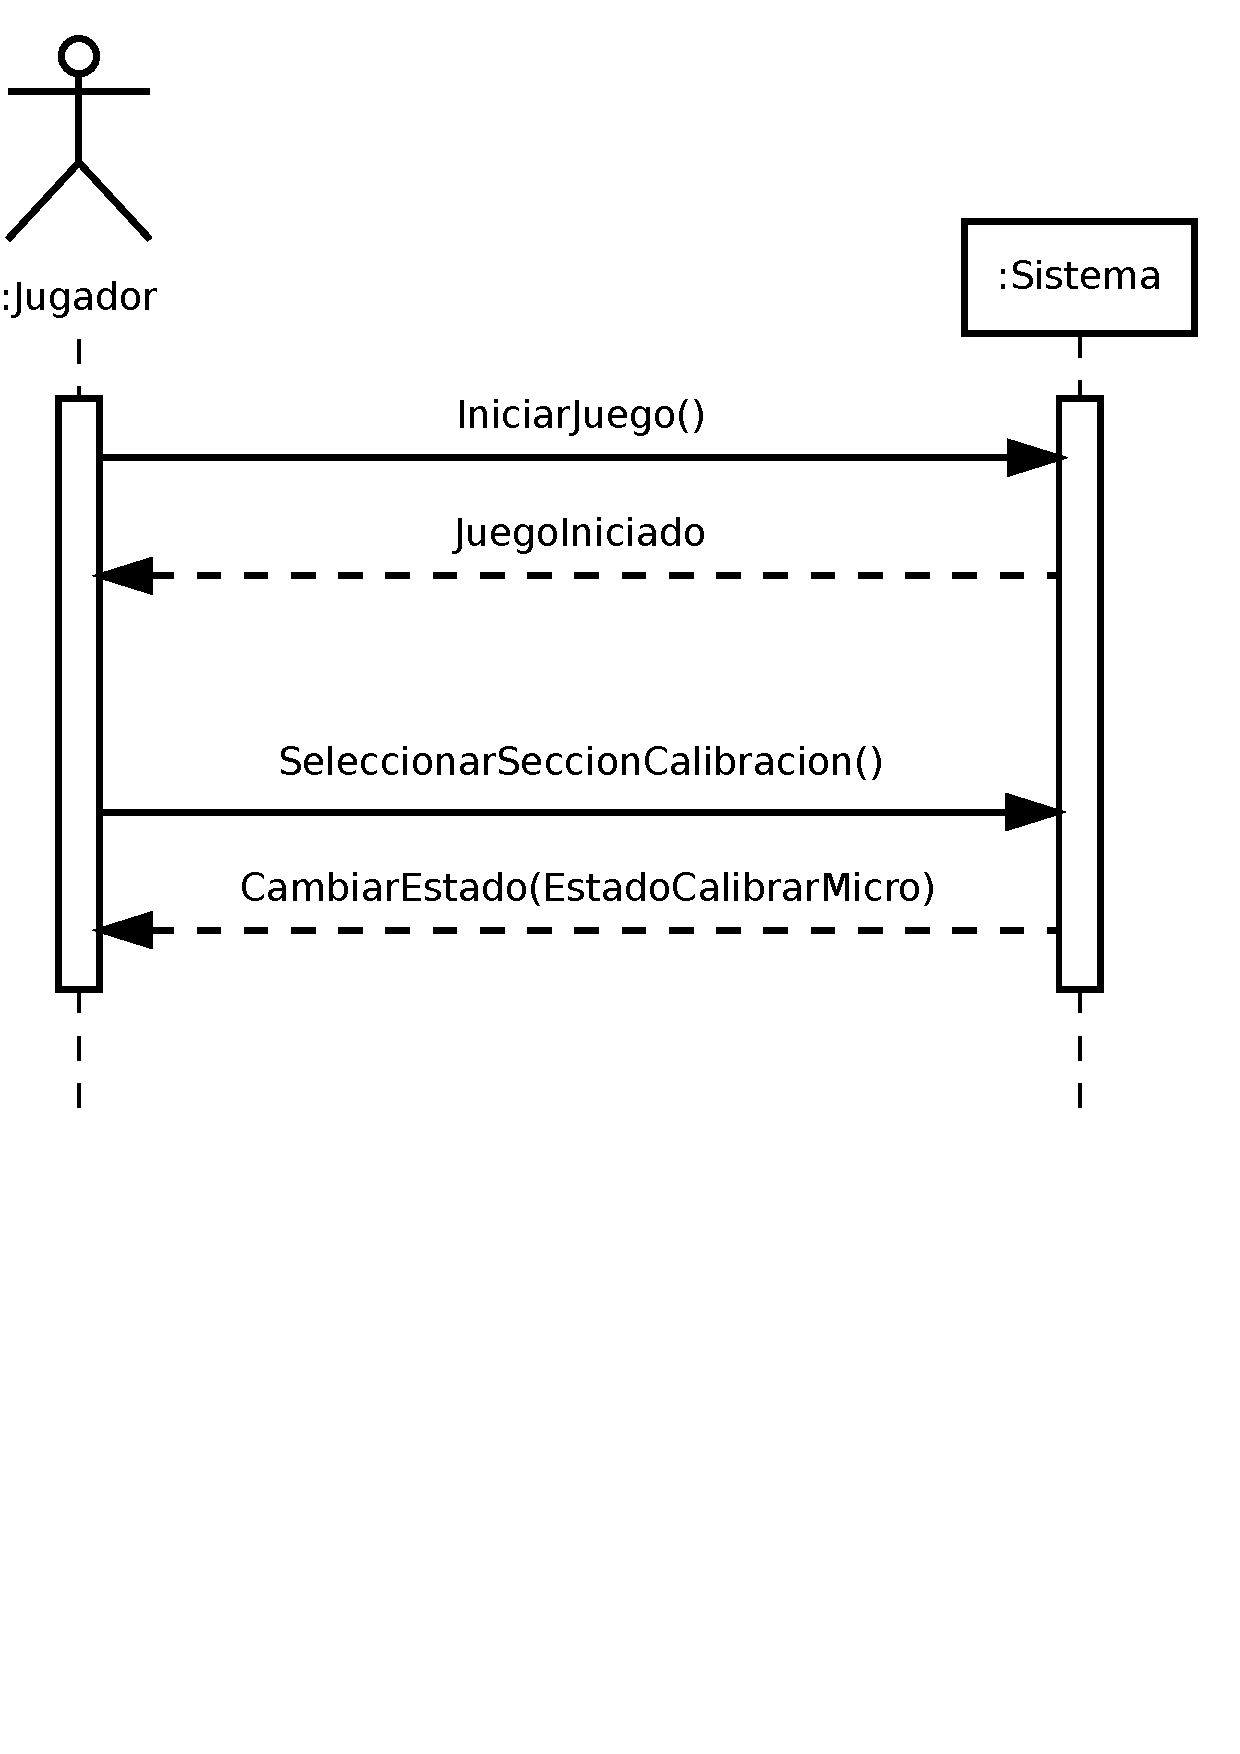
\includegraphics[trim=0cm 12cm 0cm 0cm, clip=true, width=0.5\textwidth]{4_analisis/diagsec_caso1_esc4}
  \caption{Diagrama de secuencia, incio del juego, escenario alternativo 4c}
\end{figure}

\begin{description}
\item[Operación] SeleccionarSeccionCalibracion()
\item[Actores] \jugador\, \sistema\
\item[Responsabilidades] Esconder el menú principal y cargar la sección de
  calibración de micrófono.
\item[Precondiciones] $\quad$
  \begin{itemize}
  \item El estado actual es una instancia de \textit{EstadoMenú}.
  \end{itemize}
\item[Postcondiciones] Se destruye el estado \textit{EstadoMenú} y se carga
  \textit{EstadoCalibrarMicro}.
\end{description}

\subsubsection{Escenario alternativo 4d}
\begin{figure}[h!]
  \centering
  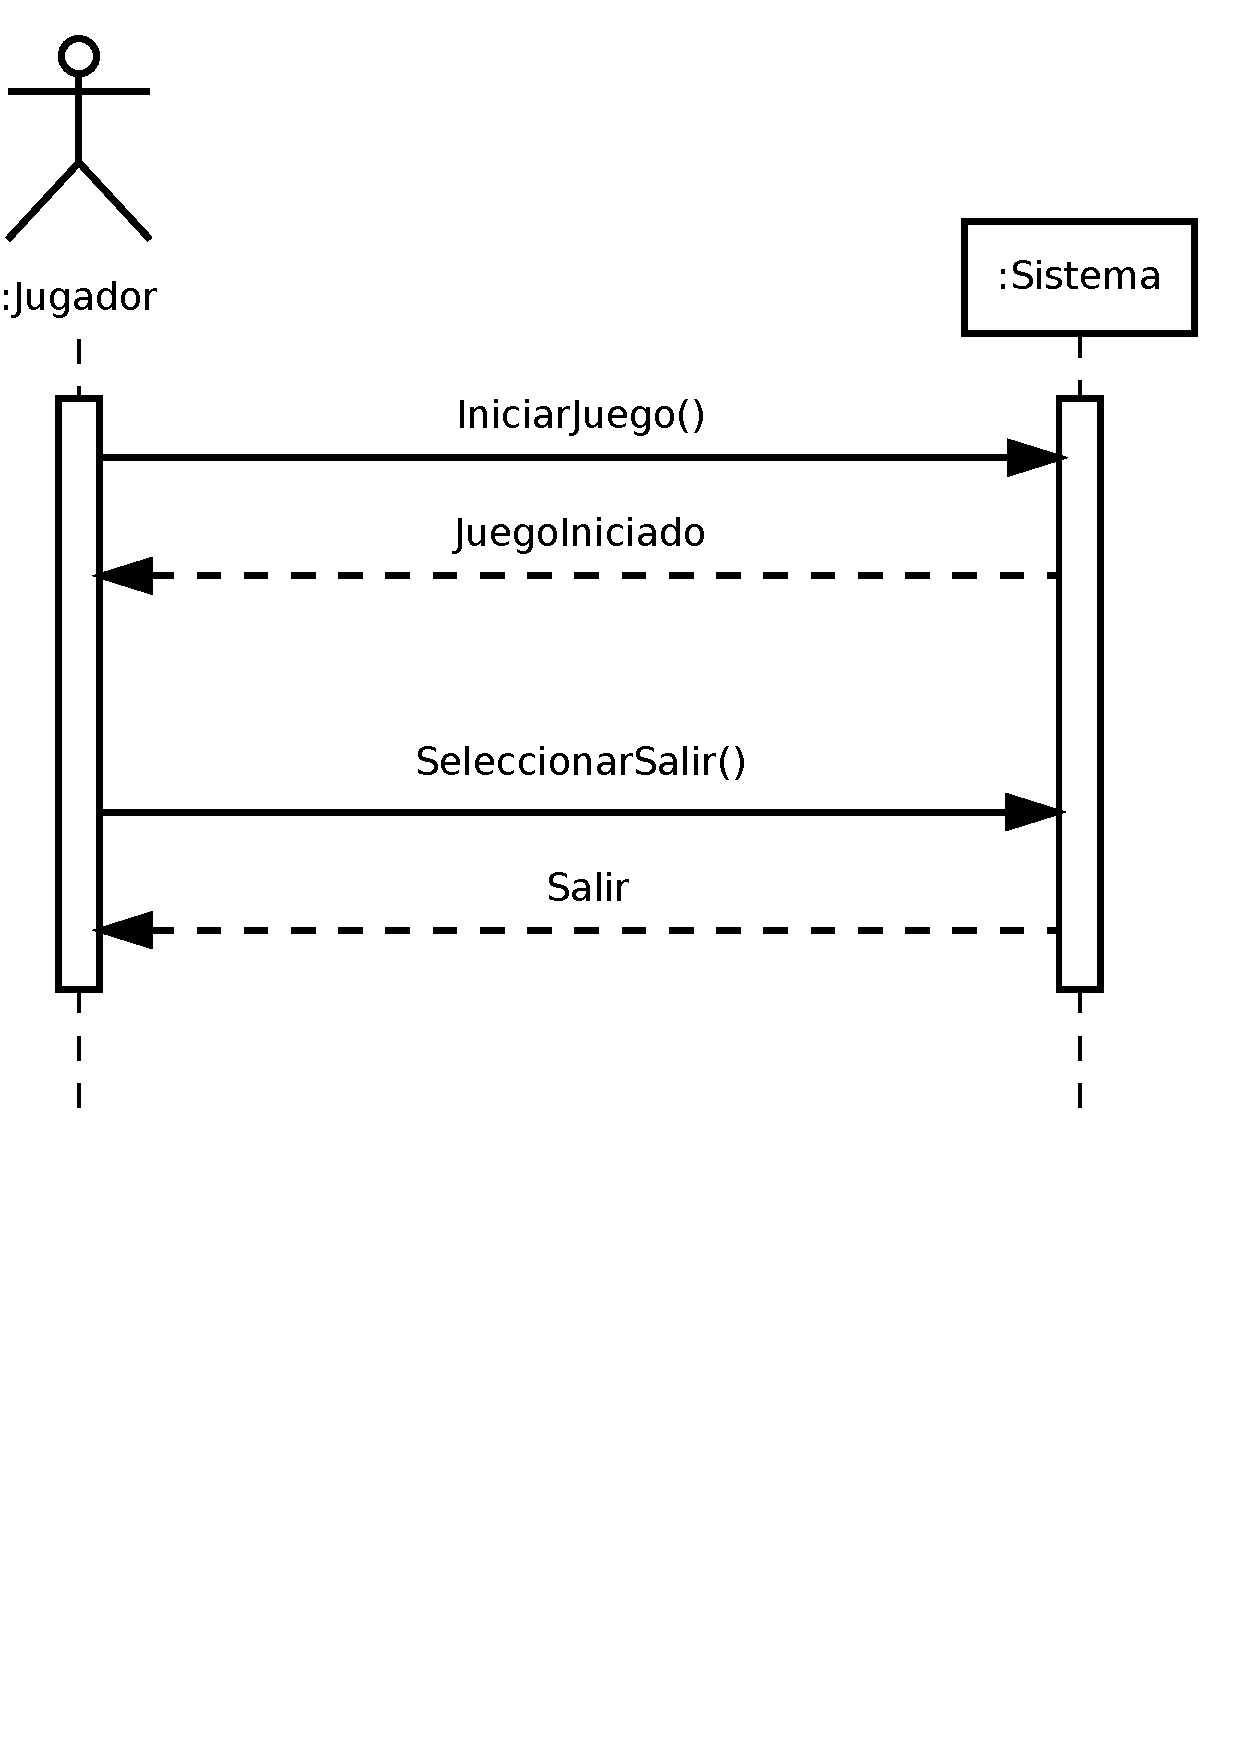
\includegraphics[trim=0cm 12cm 0cm 0cm, clip=true, width=0.5\textwidth]{4_analisis/diagsec_caso1_esc5}
  \caption{Diagrama de secuencia, incio del juego, escenario alternativo 4d}
\end{figure}

\begin{description}
\item[Operación] SeleccionarSalir()
\item[Actores] \jugador\, \sistema\
\item[Responsabilidades] Esconder el menú principal, descargar los recursos y
  cerrar la aplicación.
\item[Precondiciones] $\quad$
  \begin{itemize}
  \item El estado actual es una instancia de \textit{EstadoMenú}.
  \end{itemize}
\item[Postcondiciones] Se destruye el estado \textit{EstadoMenú}, se destruye la
  instancia de la clase \textit{Juego} y termina la ejecución de la aplicación.
\end{description}

\subsection{Selección de canción}

\subsubsection{Escenario principal}
\begin{figure}[h!]
  \centering
  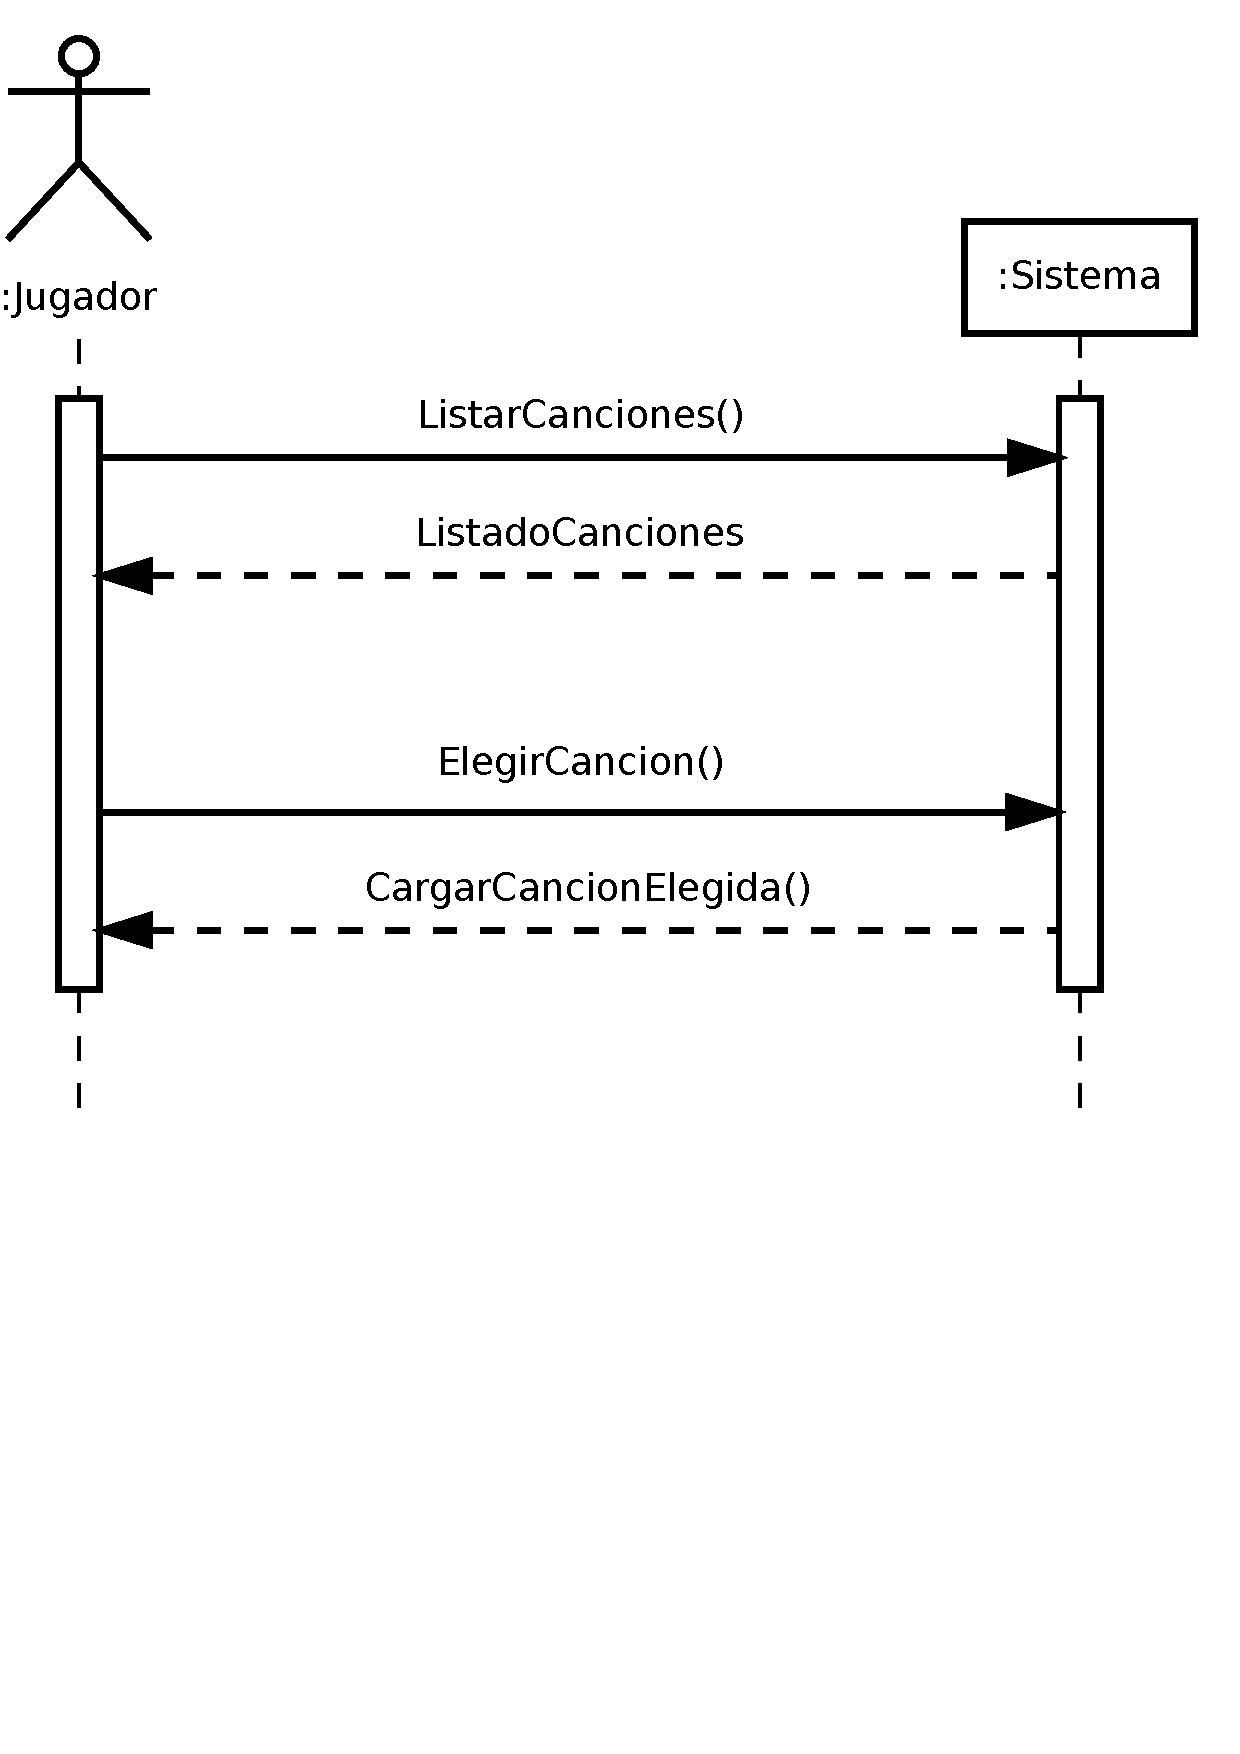
\includegraphics[trim=0cm 12cm 0cm 0cm, clip=true, width=0.5\textwidth]{4_analisis/diagsec_caso2_esc1}
  \caption{Diagrama de secuencia, selección de canción, escenario principal}
\end{figure}

\begin{description}
\item[Operación] ListarCanciones()
\item[Actores] \jugador\, \sistema\
\item[Responsabilidades] Cargar y mostrar la lista de canciones cargadas en el
  sistema.
\item[Precondiciones] Se ordenó la carga del estado \textit{EstadoMenuCanción}
\item[Postcondiciones] $\quad$
  \begin{itemize}
  \item El estado actual es una instancia de \textit{EstadoMenuCanción}.
  \item Se ha cargado la lista de canciones y se muestra en pantalla.
  \end{itemize}
\end{description}

\begin{description}
\item[Operación] ElegirCanción()
\item[Actores] \jugador\, \sistema\
\item[Responsabilidades] Cargar la canción que el usuario ha elegido para
  interpretar.
\item[Precondiciones] Existe una lista de canciones cargada de entre las que el
  usuario ha elegido una.
\item[Postcondiciones] $\quad$
  \begin{itemize}
  \item Se carga la canción indicada.
  \item Se oculta la lista de canciones.
  \item Se pasa a un sub-estado de interpretación de canción.
  \end{itemize}
\end{description}
\subsubsection{Escenario alternativo 3a}
\begin{figure}[h!]
  \centering
  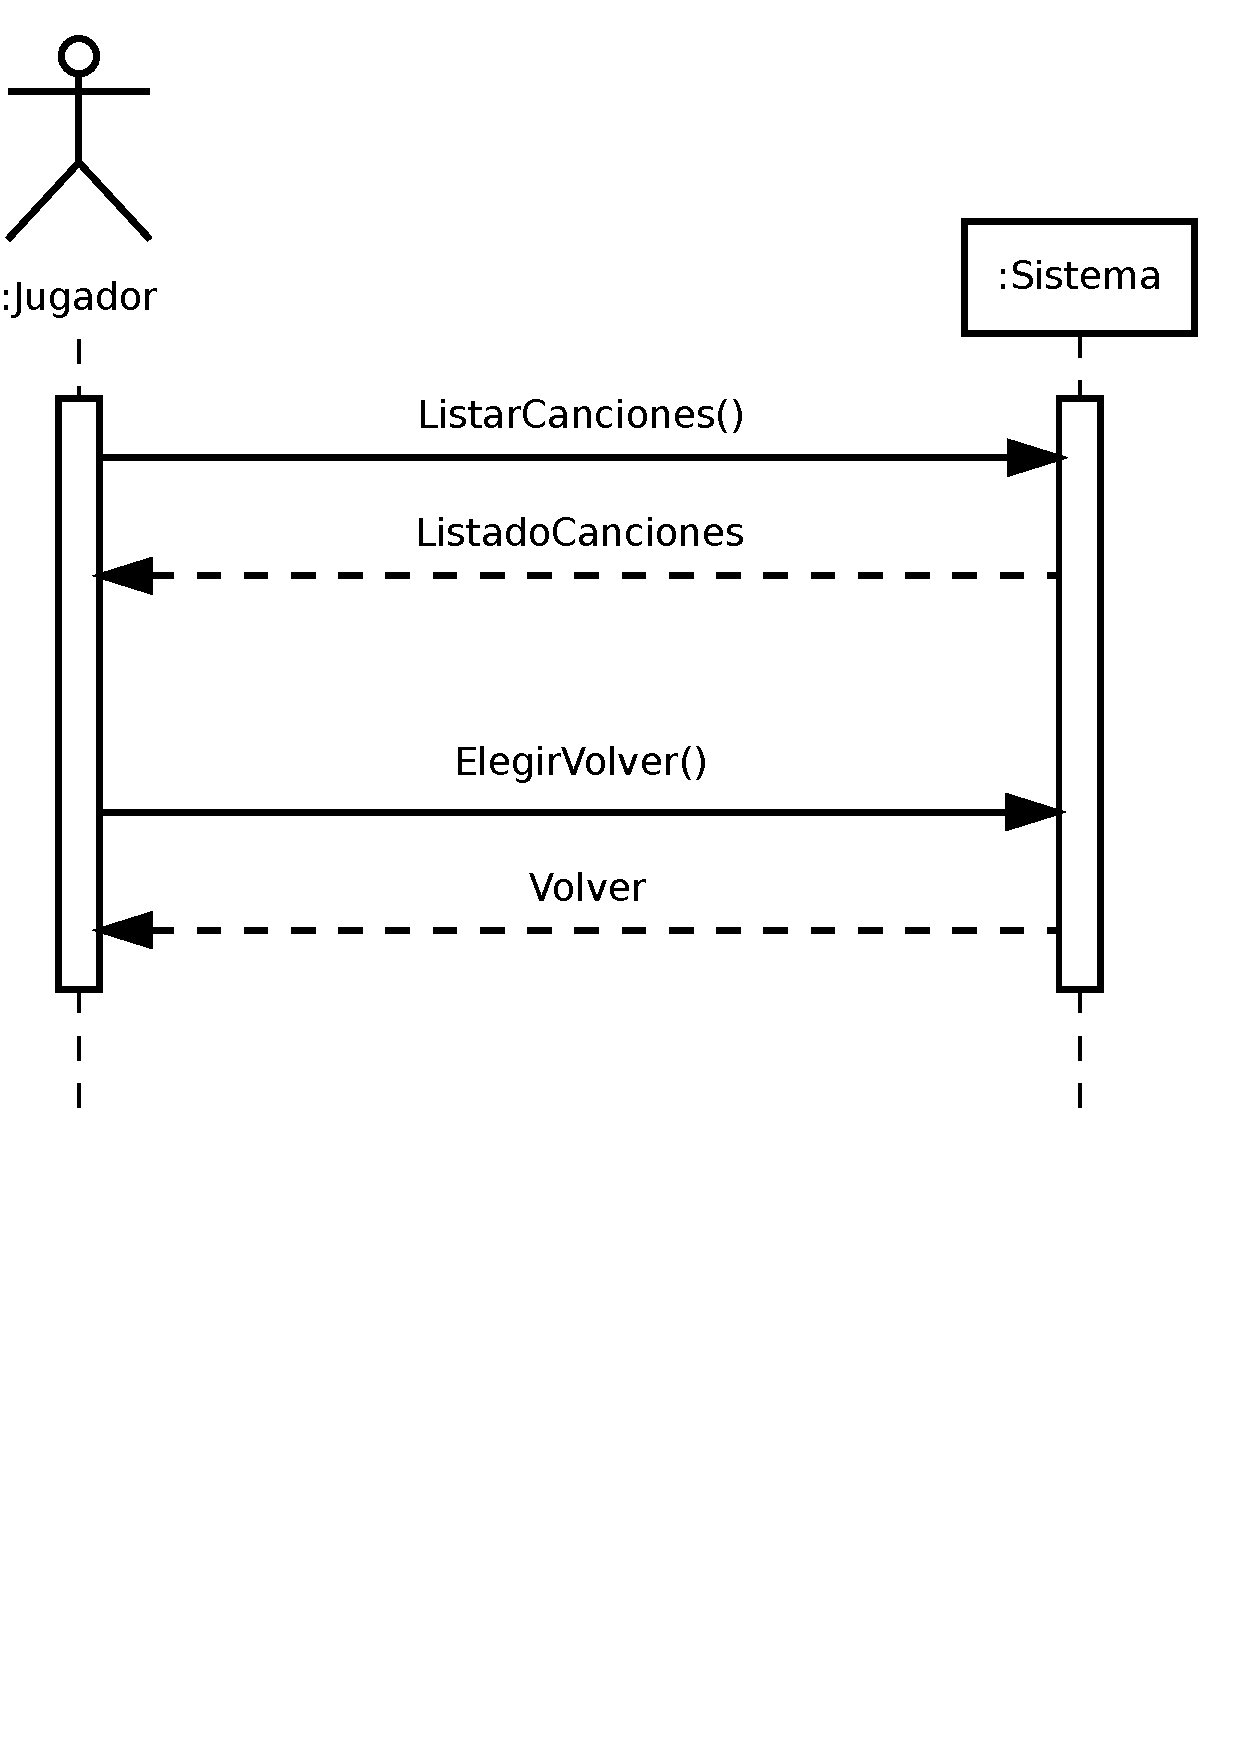
\includegraphics[trim=0cm 12cm 0cm 0cm, clip=true, width=0.5\textwidth]{4_analisis/diagsec_caso2_esc2}
  \caption{Diagrama de secuencia, selección de canción, escenario alternativo 3a}
\end{figure}
\begin{description}
\item[Operación] ElegirVolver()
\item[Actores] \jugador\, \sistema\
\item[Responsabilidades] Descargar la sección actual y volver al menú anterior.
\item[Precondiciones] El estado actual es una instancia de \textit{EstadoMenuCanción}.
\item[Postcondiciones] $\quad$
  \begin{itemize}
  \item El estado instancia de \textit{EstadoMenuCanción} queda descargado.
  \item Se carga y se muestra \textit{EstadoMenú}.
  \end{itemize}
\end{description}

\subsection{Interpretación de canción}
\begin{nota}
  No se reflejan los escenarios alternativos al estar englobados en la operación
  \textit{InteractuarConFlauta}.
\end{nota}

\subsubsection{Escenario principal}
\begin{figure}[h!]
  \centering
  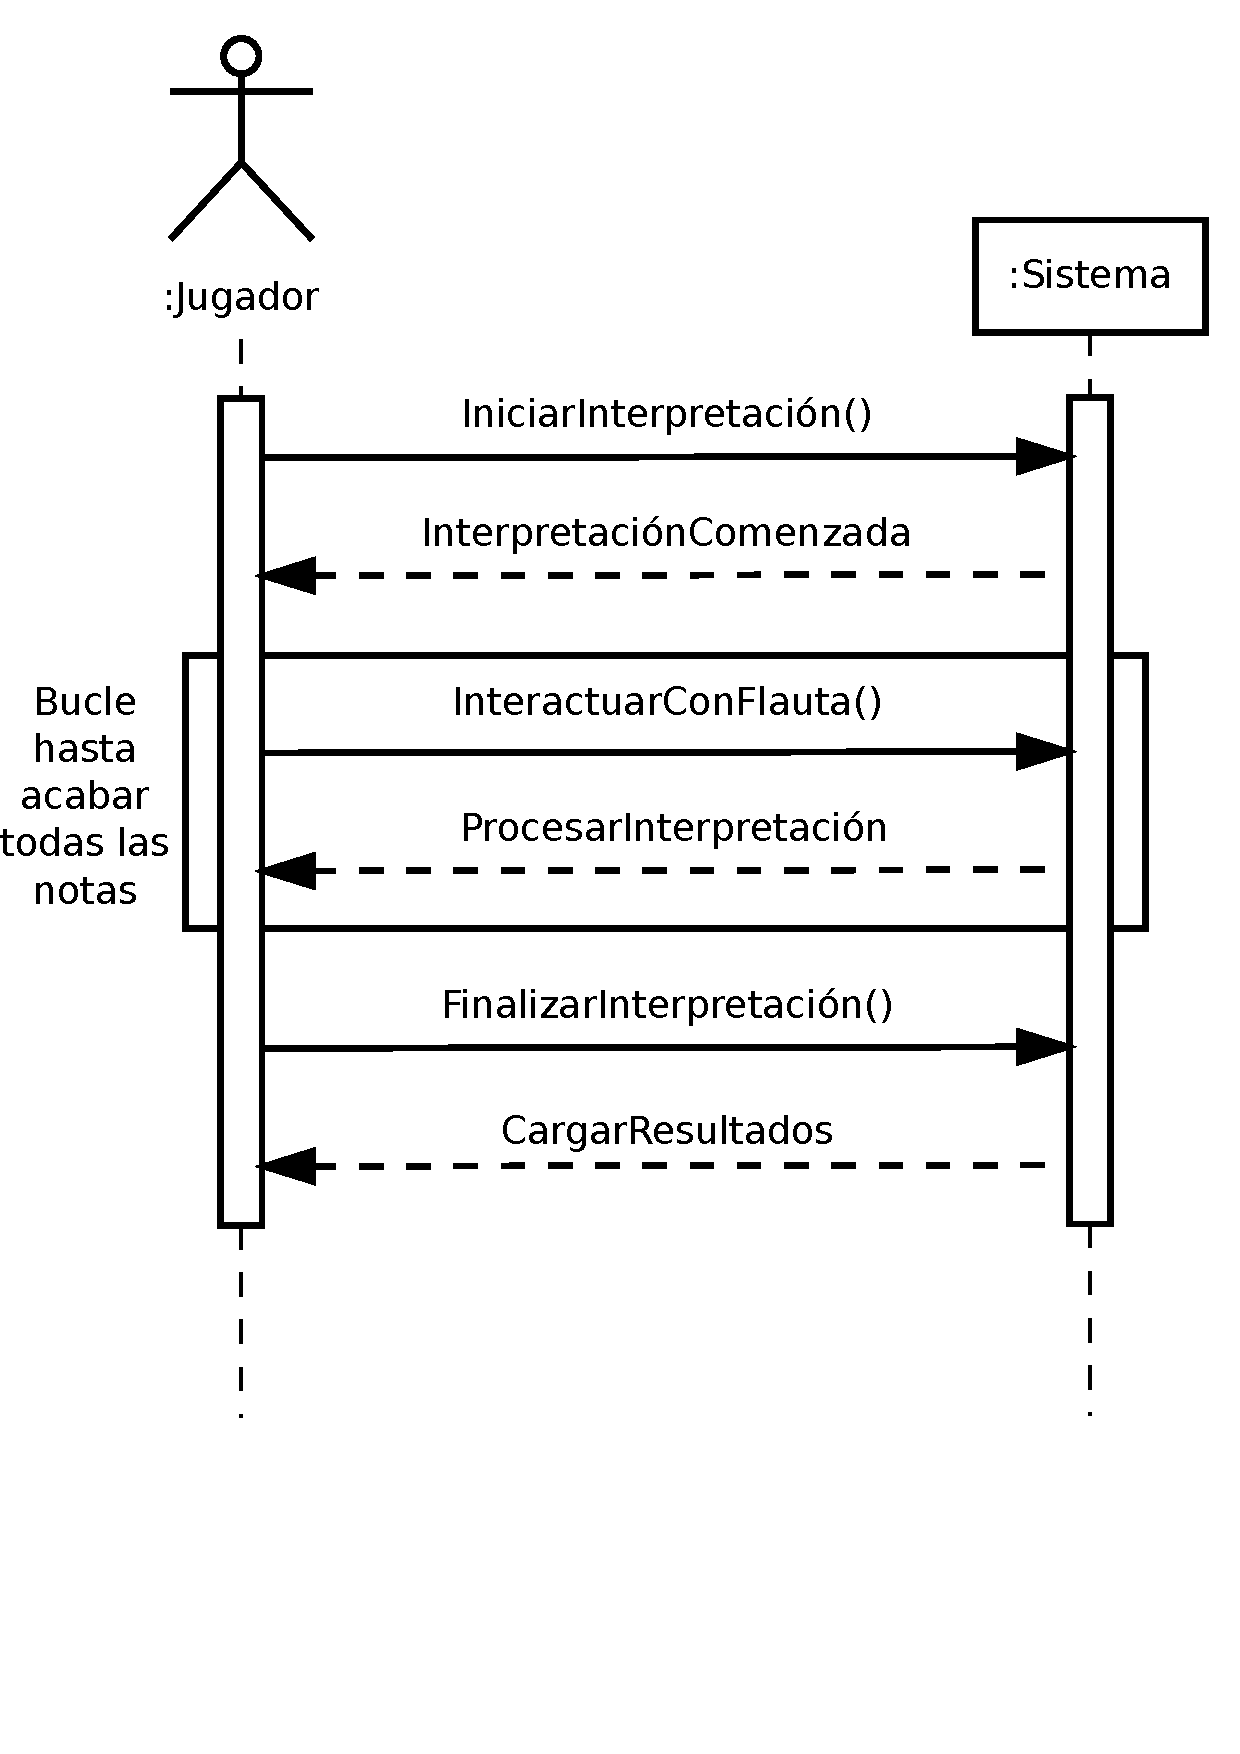
\includegraphics[trim=0cm 8cm 0cm 0cm, clip=true, width=0.5\textwidth]{4_analisis/diagsec_caso3}
  \caption{Diagrama de secuencia, interpretación de canción, escenario principal}
\end{figure}

\begin{description}
\item[Operación] IniciarInterpretación()
\item[Actores] \jugador\, \sistema\
\item[Responsabilidades] Parsear el fichero de canción, cargar la interfaz y
  comenzar la interpretación.
\item[Precondiciones] El usuario ha elegido una canción en el estado anterior.
\item[Postcondiciones] $\quad$
  \begin{itemize}
  \item Se muestra la interfaz de interpretación de canción.
  \item El fichero de canción queda cargado e interpretado, instanciando los
    elementos de la clase \textit{Nota} que sean necesarios.
  \item Comienza la interpretación
  \end{itemize}
\end{description}

\begin{description}
\item[Operación] InteractuarConFlauta()
\item[Actores] \jugador\, \sistema\
\item[Responsabilidades] El \jugador\ interactúa con el sistema mediante la
  flauta a través del micrófono, y el \sistema\ analiza los datos y muestra una
  respuesta en pantalla.
\item[Precondiciones] $\quad$
  \begin{itemize}
  \item La interpretación ha comenzado.
  \item El micrófono está correctamente configurado.
  \end{itemize}
\item[Postcondiciones] $\quad$
  \begin{itemize}
  \item El sistema captura y analiza los datos de audio.
  \item Según el análisis, el sistema responde de una forma u otra (según los
    escenarios alternativos 3a, 4a y 5a del caso de uso \textit{interpretación
      de canción}).
  \end{itemize}
\end{description}

\begin{description}
\item[Operación] FinalizarInterpretación()
\item[Actores] \jugador\, \sistema\
\item[Responsabilidades] Descargar la pantalla de interpretación, descargar la
  canción y finalizar la interpretación.
\item[Precondiciones] Todas las notas se han interpretado.
\item[Postcondiciones] $\quad$
  \begin{itemize}
  \item Se descarga la \textit{Canción} actual.
  \item Se ocultan los elementos de la interfaz de interpretación.
  \item Se lanza la sección de puntuación.
  \end{itemize}
\end{description}


\subsection{Resultados de interpretación}

\subsubsection{Escenario principal}
\begin{figure}[h!]
  \centering
  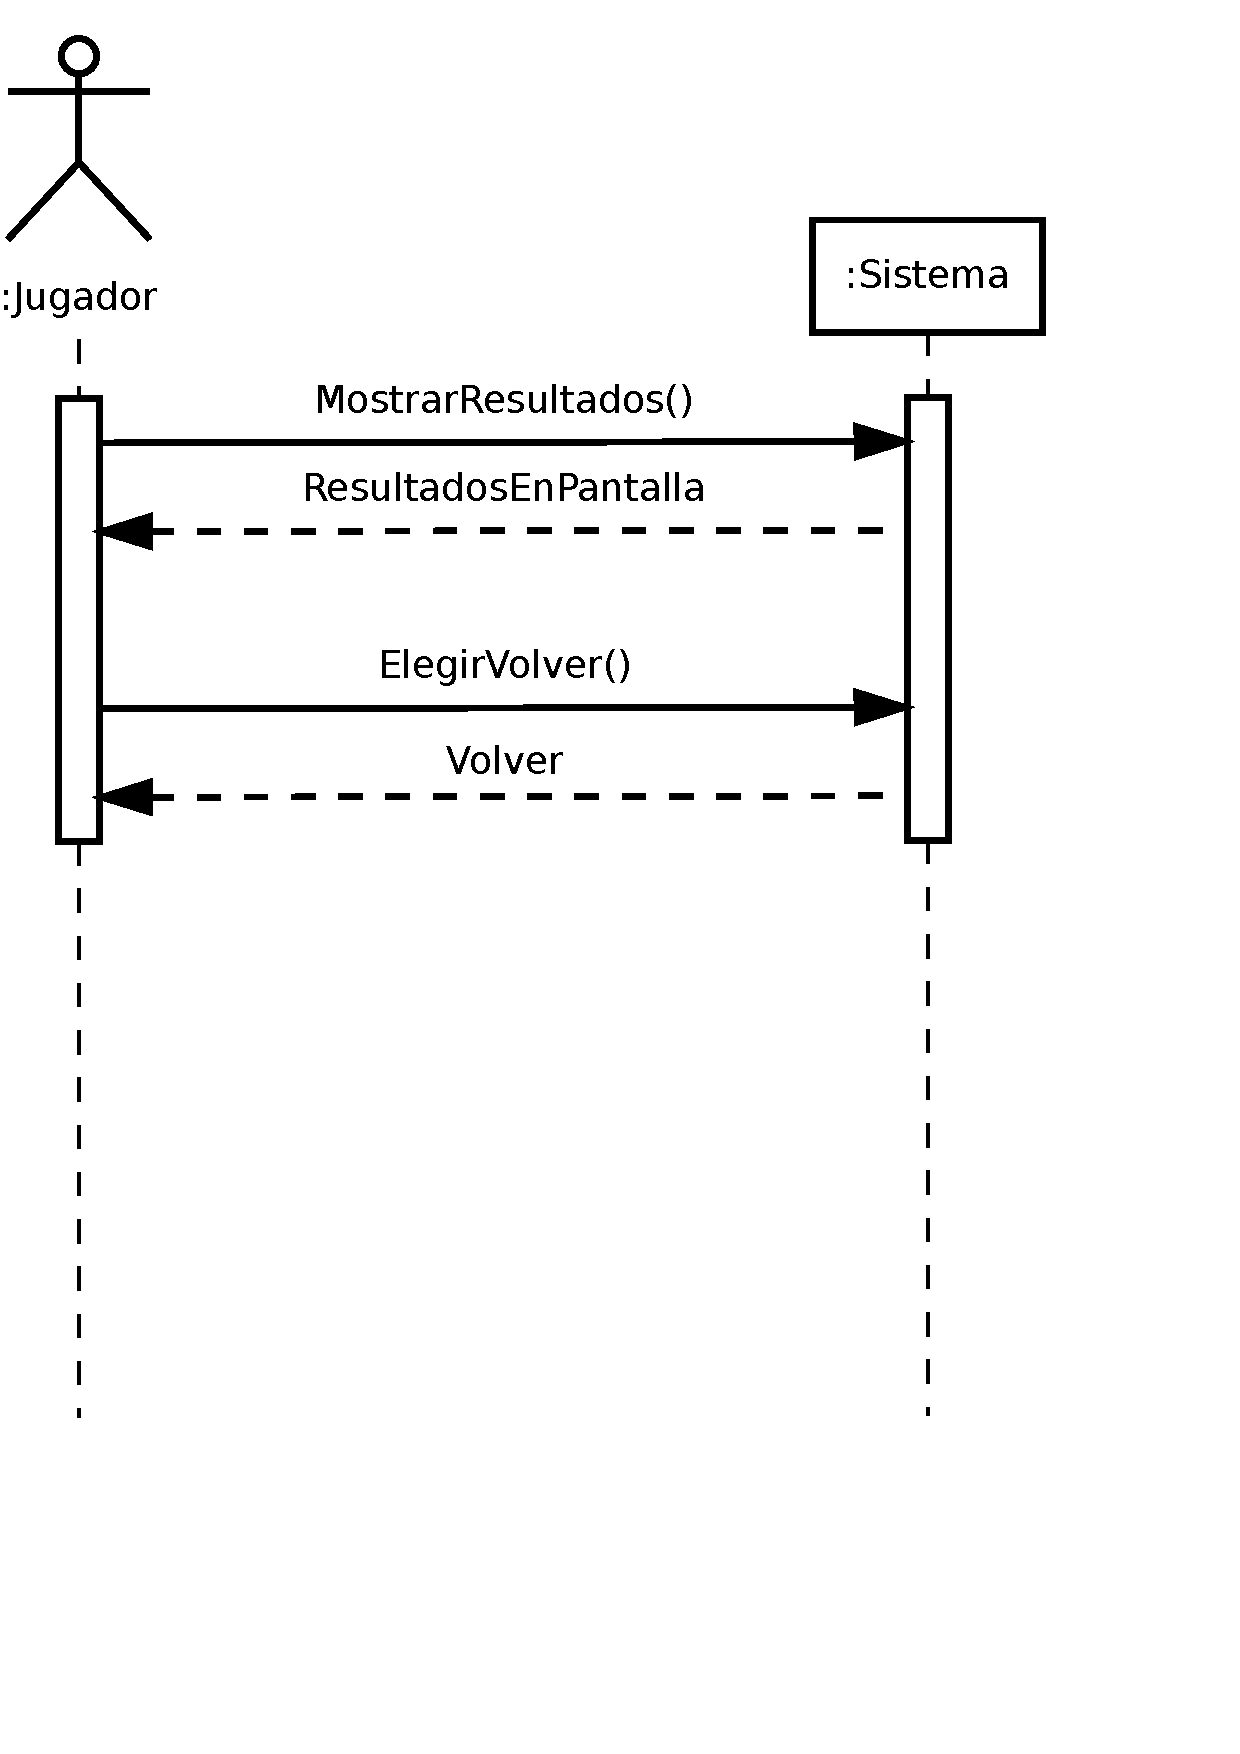
\includegraphics[trim=0cm 12cm 0cm 0cm, clip=true, width=0.5\textwidth]{4_analisis/diagsec_caso4}
  \caption{Diagrama de secuencia, resultados de interpretación, escenario principal}
\end{figure}

\begin{description}
\item[Operación] MostrarResultados()
\item[Actores] \jugador\, \sistema\
\item[Responsabilidades] Interpretar los resultados de la interpretación y
  mostrar los resultados en pantalla.
\item[Precondiciones] El \jugador\ ha concluído satisfactoriamente una
  interpretación completa de una canción, obteniendo una suma de puntos $X$.
\item[Postcondiciones] Mostrar en pantalla los resultados en forma de porcentaje
  de aciertos, y un mensaje según aquél.
\end{description}

\begin{description}
\item[Operación] ElegirVolver()
\item[Actores] \jugador\, \sistema\
\item[Responsabilidades] Descargar la sección actual y volver al menú anterior.
\item[Precondiciones] $\quad$
  \begin{itemize}
  \item La aplicación se encuentra en la pantalla de muestra de resultados.
  \item El usuario ha pulsado la tecla \texttt{escape} o el botón \textit{volver}.
  \end{itemize}
\item[Postcondiciones] $\quad$
  \begin{itemize}
  \item Se descargan todos los datos referentes a la canción actual.
  \item Se carga y se muestra \textit{EstadoMenúCanciones}.
  \end{itemize}
\end{description}

\subsection{Analizador de notas}

\begin{nota}
  No se reflejan los escenarios alternativos al estar englobados en la operación
  \textit{InteractuarConFlauta}.
\end{nota}

\subsubsection{Escenario principal}
\begin{figure}[h!]
  \centering
  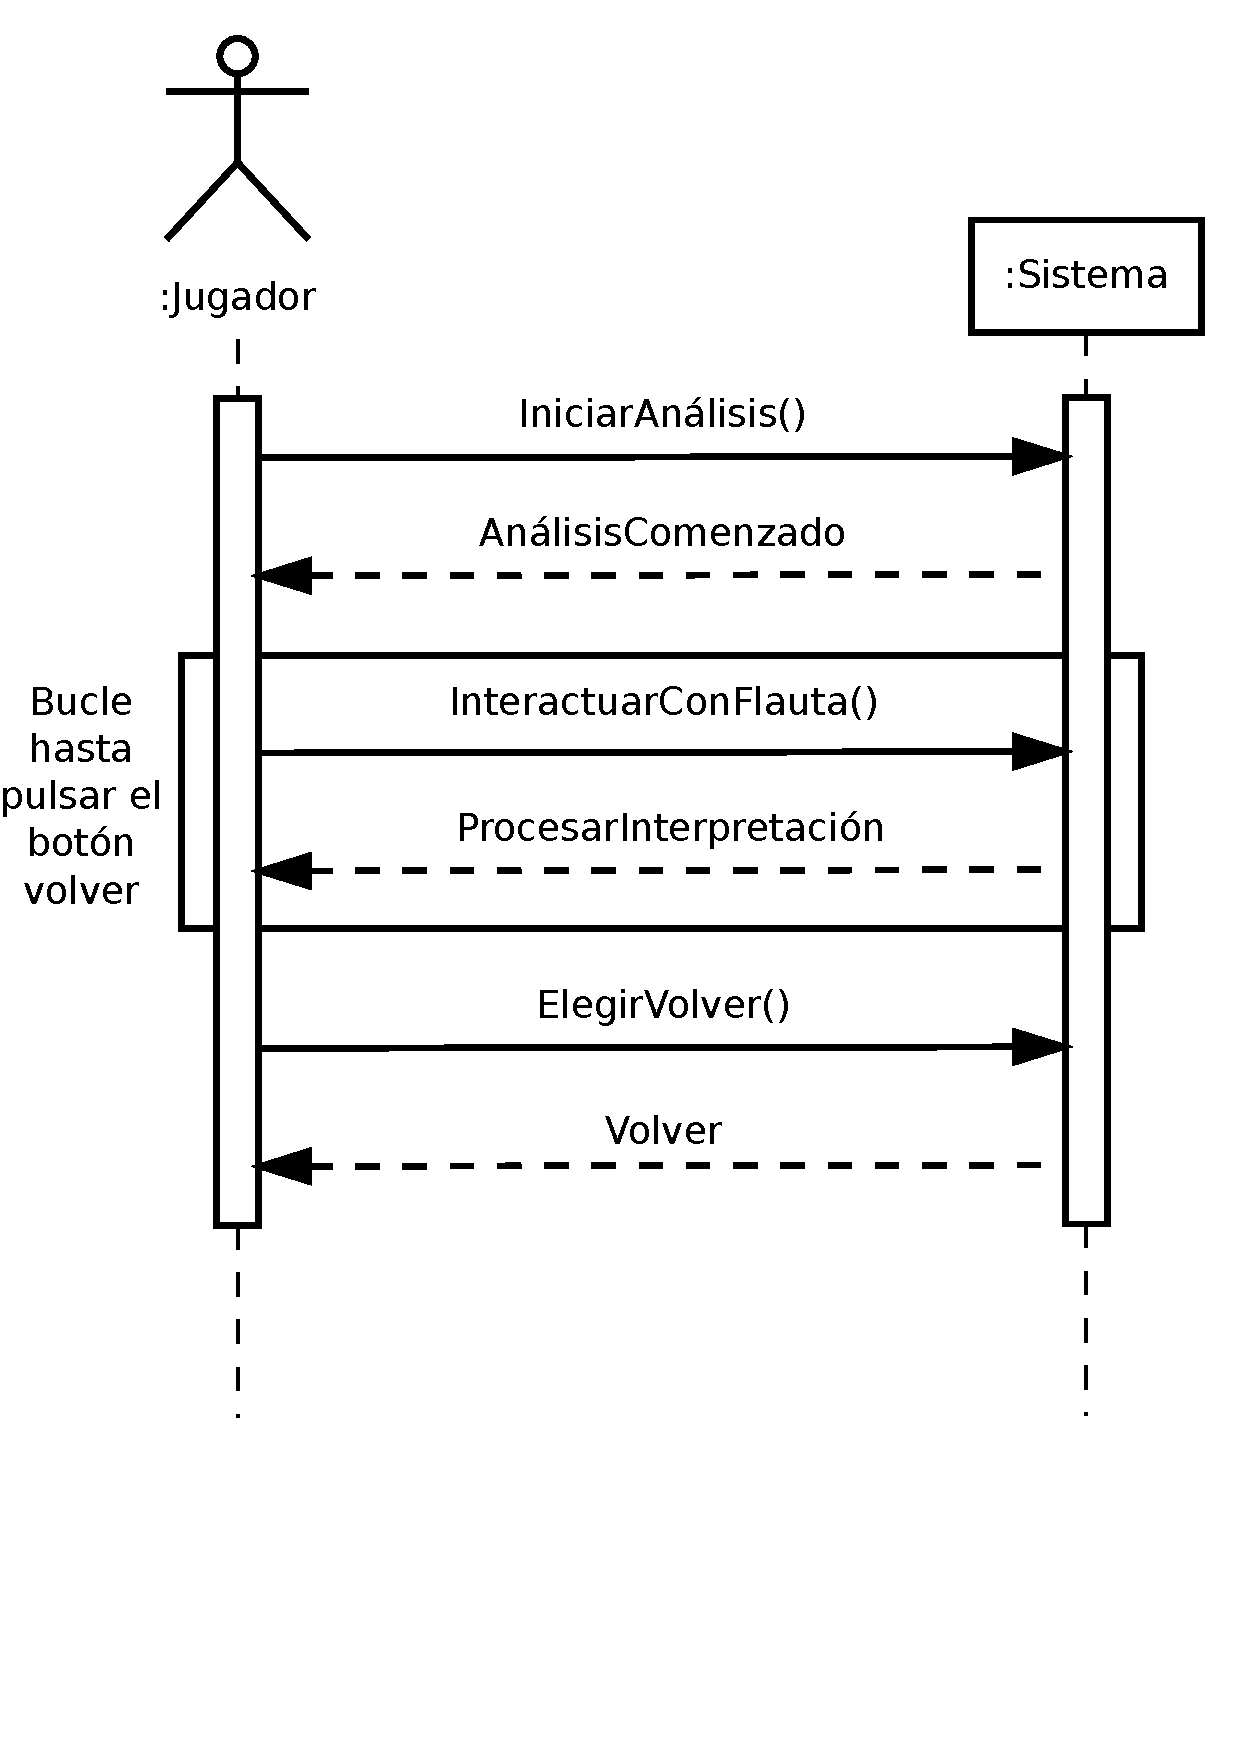
\includegraphics[trim=0cm 8cm 0cm 0cm, clip=true, width=0.5\textwidth]{4_analisis/diagsec_caso5}
  \caption{Diagrama de secuencia, interpretación de canción, escenario principal}
\end{figure}

\begin{description}
\item[Operación] IniciarAnálisis
\item[Actores] \jugador\, \sistema\
\item[Responsabilidades] Cargar la interfaz e iniciar el análisis de notas.
\item[Precondiciones] El usuario eligió la sección \textit{Analizador de notas}
  en el menú principal.
\item[Postcondiciones] $\quad$
  \begin{itemize}
  \item Aparece la interfaz del analizador de notas.
  \item Se inicia el análisis de notas
  \end{itemize}
\end{description}

\begin{description}
\item[Operación] InteractuarConFlauta
\item[Actores] \jugador\, \sistema\
\item[Responsabilidades] El \jugador\ toca notas en la flauta y el \sistema\
  captura y reconoce el audio, indicando la nota tocada en pantalla.

\item[Precondiciones] Se ha iniciado el análisis.

\item[Postcondiciones] $\quad$
  \begin{itemize}
  \item El \sistema\ recoge y analiza el sonido que emite la flauta del \jugador.
  \item El \sistema\ representa en pantalla la nota identificada, o no muestra
    nada en caso de identificación defectuosa.
  \end{itemize}
\end{description}

% \begin{description}
% \item[Operación] ElegirVolver()
% \item[Actores] \jugador\, \sistema\
% \item[Responsabilidades] Descargar la sección actual y volver al menú anterior.
% \item[Precondiciones] $\quad$
%   \begin{itemize}
%   \item El estado actual es una instancia de \textit{EstadoAnalizador}.
%   \item Hay un análisis en curso.  
%   \end{itemize}
  
% \item[Postcondiciones] $\quad$
%   \begin{itemize}
%   \item Concluye el análisis actual.
%   \item Se destruye el estado.
%   \item Se carga y se muestra \textit{EstadoMenú}.
%   \end{itemize}
% \end{description}

\subsection{Calibración de micrófono}

\subsubsection{Escenario principal}
\begin{figure}[h!]
  \centering
  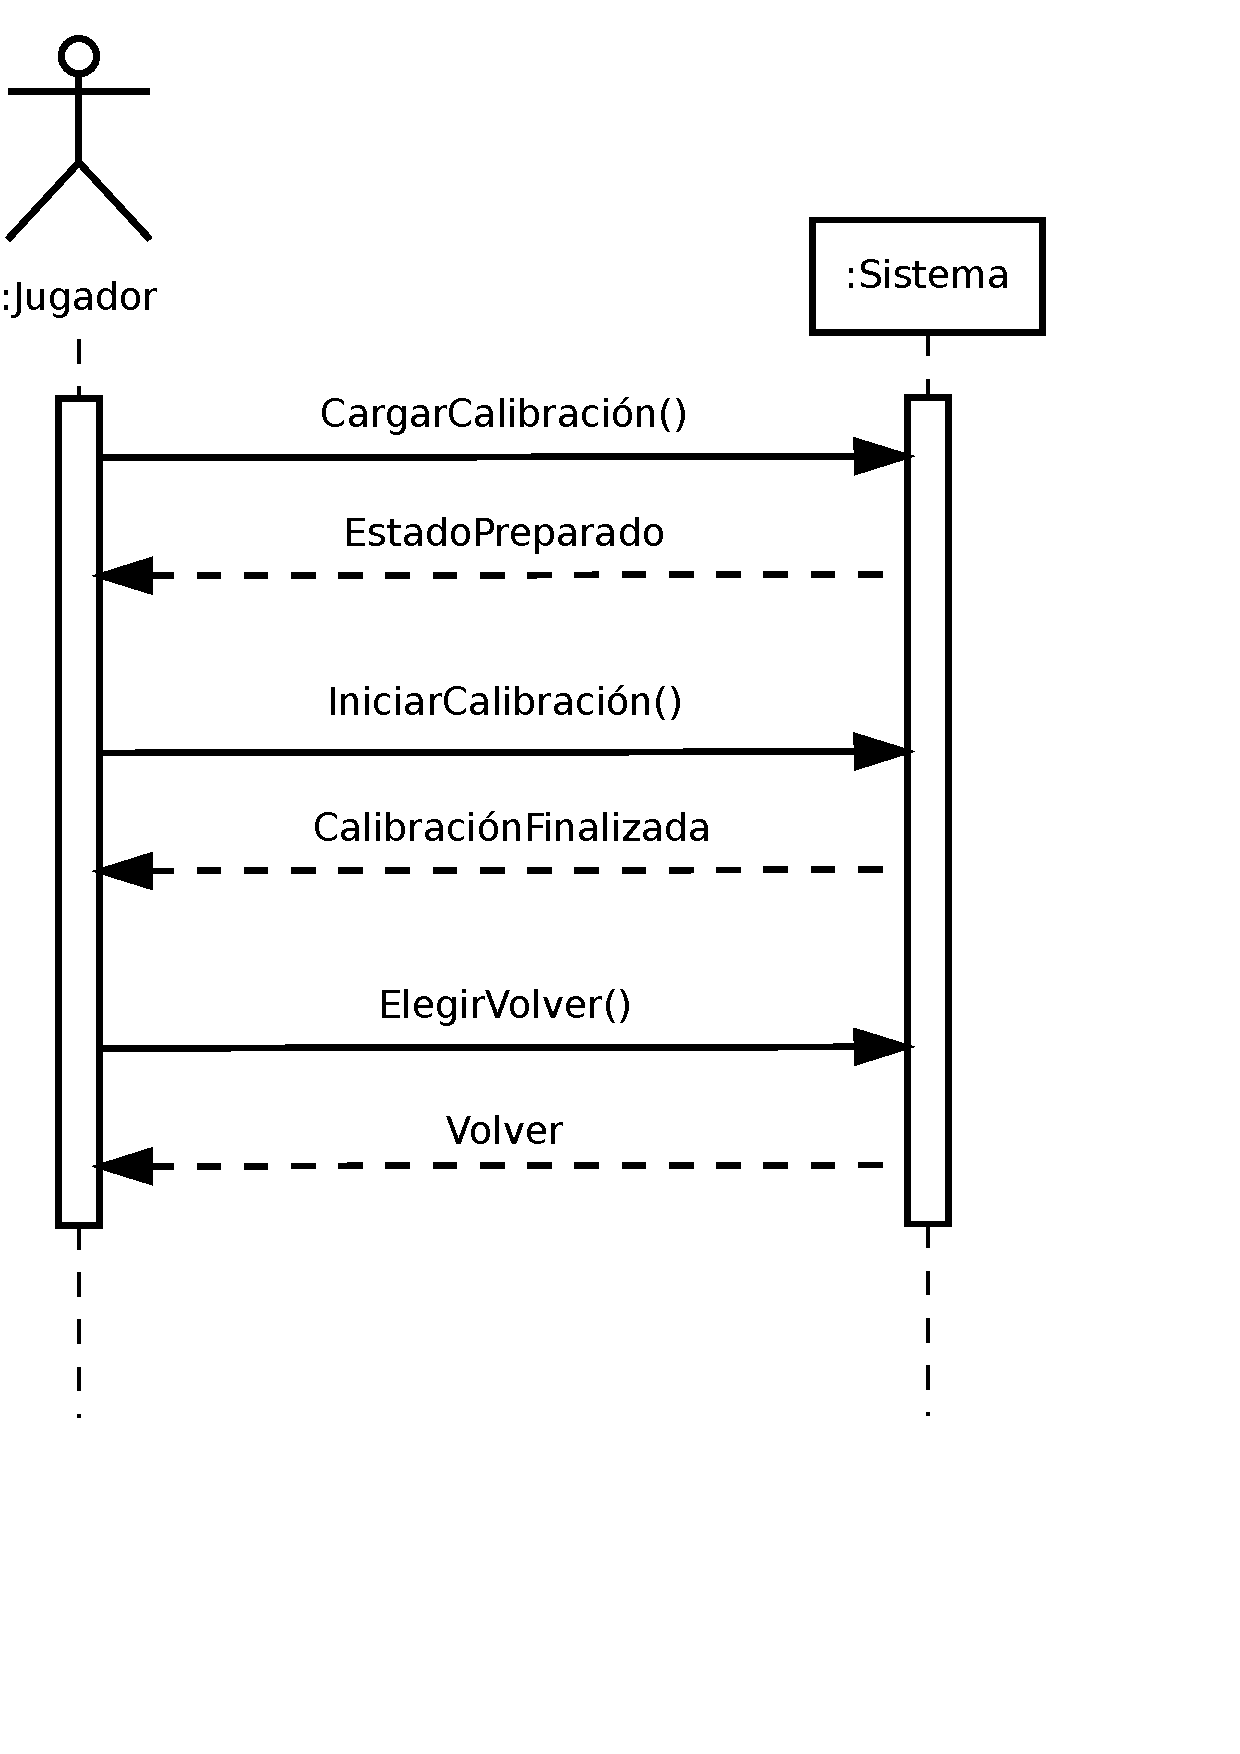
\includegraphics[trim=0cm 8cm 0cm 0cm, clip=true, width=0.5\textwidth]{4_analisis/diagsec_caso6_esc1}
  \caption{Diagrama de secuencia, calibración de micrófono, escenario principal}
\end{figure}

\begin{description}
\item[Operación] CargarCalibración()
\item[Actores] \jugador\, \sistema\
\item[Responsabilidades] Cargar la sección y preparar el sistema para comenzar
  la calibración del micrófono.
\item[Precondiciones] El usuario ha elegido en el menú principal la opción
  \textit{Calibrar micrófono}.
\item[Postcondiciones] La sección está cargada y la calibración lista para
  iniciarse.
\end{description}

\begin{description}
\item[Operación] CalibrarMicrófono()
\item[Actores] \jugador\, \sistema\
\item[Responsabilidades] Llevar a cabo la calibración correcta del micrófono.
\item[Precondiciones] El usuario ha lanzado la calibración del micrófono.
\item[Postcondiciones] $\quad$
  \begin{itemize}
  \item Se cierra el sistema de sonido.
  \item Se obtiene un valor umbral de ruido ambiente, fruto de una calibración
    exitosa.
  \end{itemize}
\end{description}

\begin{description}
\item[Operación] ElegirVolver()
\item[Actores] \jugador\, \sistema\
\item[Responsabilidades] Descargar la sección actual y volver al menú anterior.
\item[Precondiciones] $\quad$
  \begin{itemize}
  \item La calibración ha concluído exitosamente.
  \item El usuario ha pulsado la tecla \texttt{escape} o el botón \textit{volver}.
  \end{itemize}
\item[Postcondiciones] $\quad$
  \begin{itemize}
  \item Se descarga la sección actual.
  \item Se carga y se muestra \textit{EstadoMenúCanciones}.
  \end{itemize}
\end{description}

\subsubsection{Escenario alternativo 5a}
\begin{figure}[h!]
  \centering
  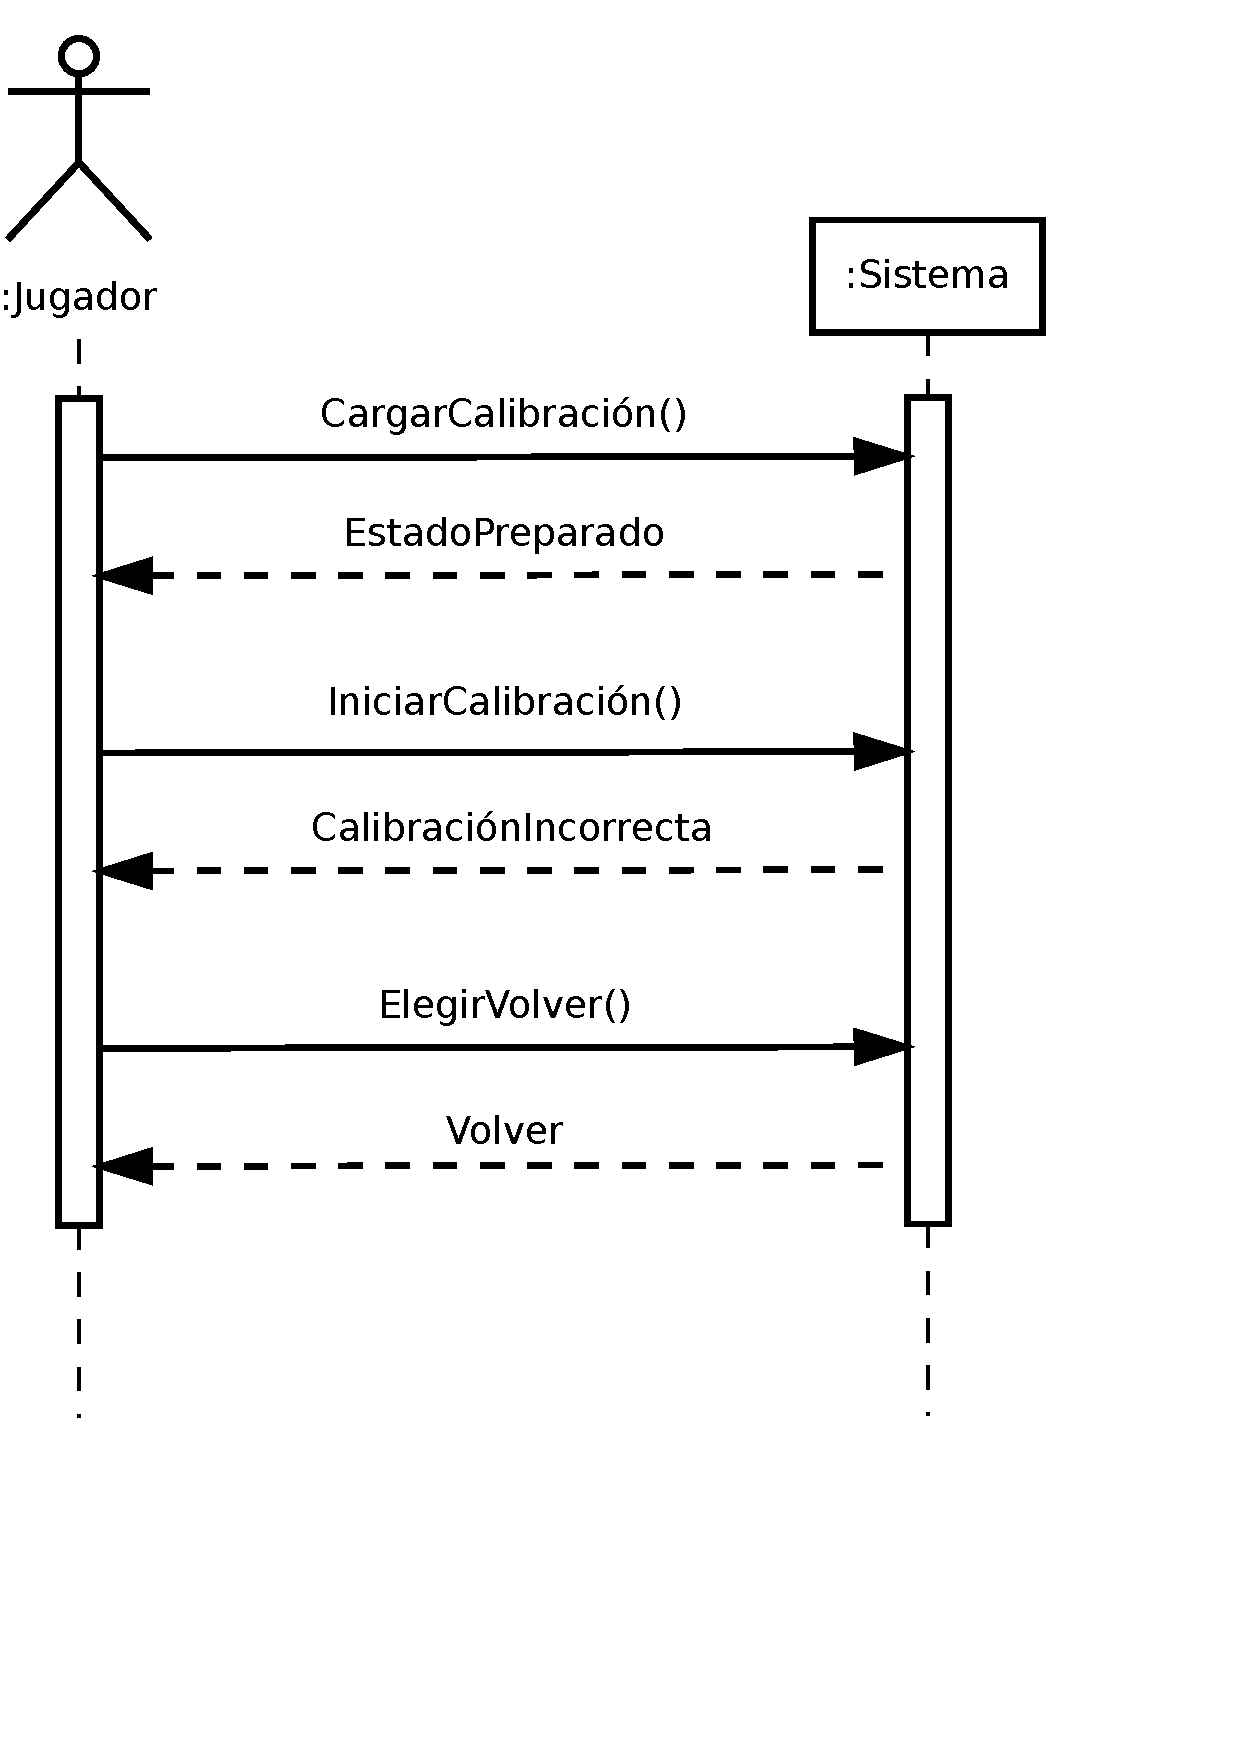
\includegraphics[trim=0cm 8cm 0cm 0cm, clip=true, width=0.5\textwidth]{4_analisis/diagsec_caso6_esc2}
  \caption{Diagrama de secuencia, calibración de micrófono, escenario principal}
\end{figure}
\begin{description}
\item[Operación] CalibrarMicrófono()
\item[Actores] \jugador\, \sistema\
\item[Responsabilidades] Llevar a cabo la calibración correcta del micrófono.
\item[Precondiciones] El usuario ha lanzado la calibración del micrófono.
\item[Postcondiciones] $\quad$
  \begin{itemize}
  \item Se cierra el sistema de sonido.
  \item La calibración ha fallado.
  \item No se obtiene valor umbral de ruido ambiental.
  \end{itemize}
\end{description}

\subsection{Selección de lecciones}

\subsubsection{Escenario principal}
\begin{figure}[h!]
  \centering
  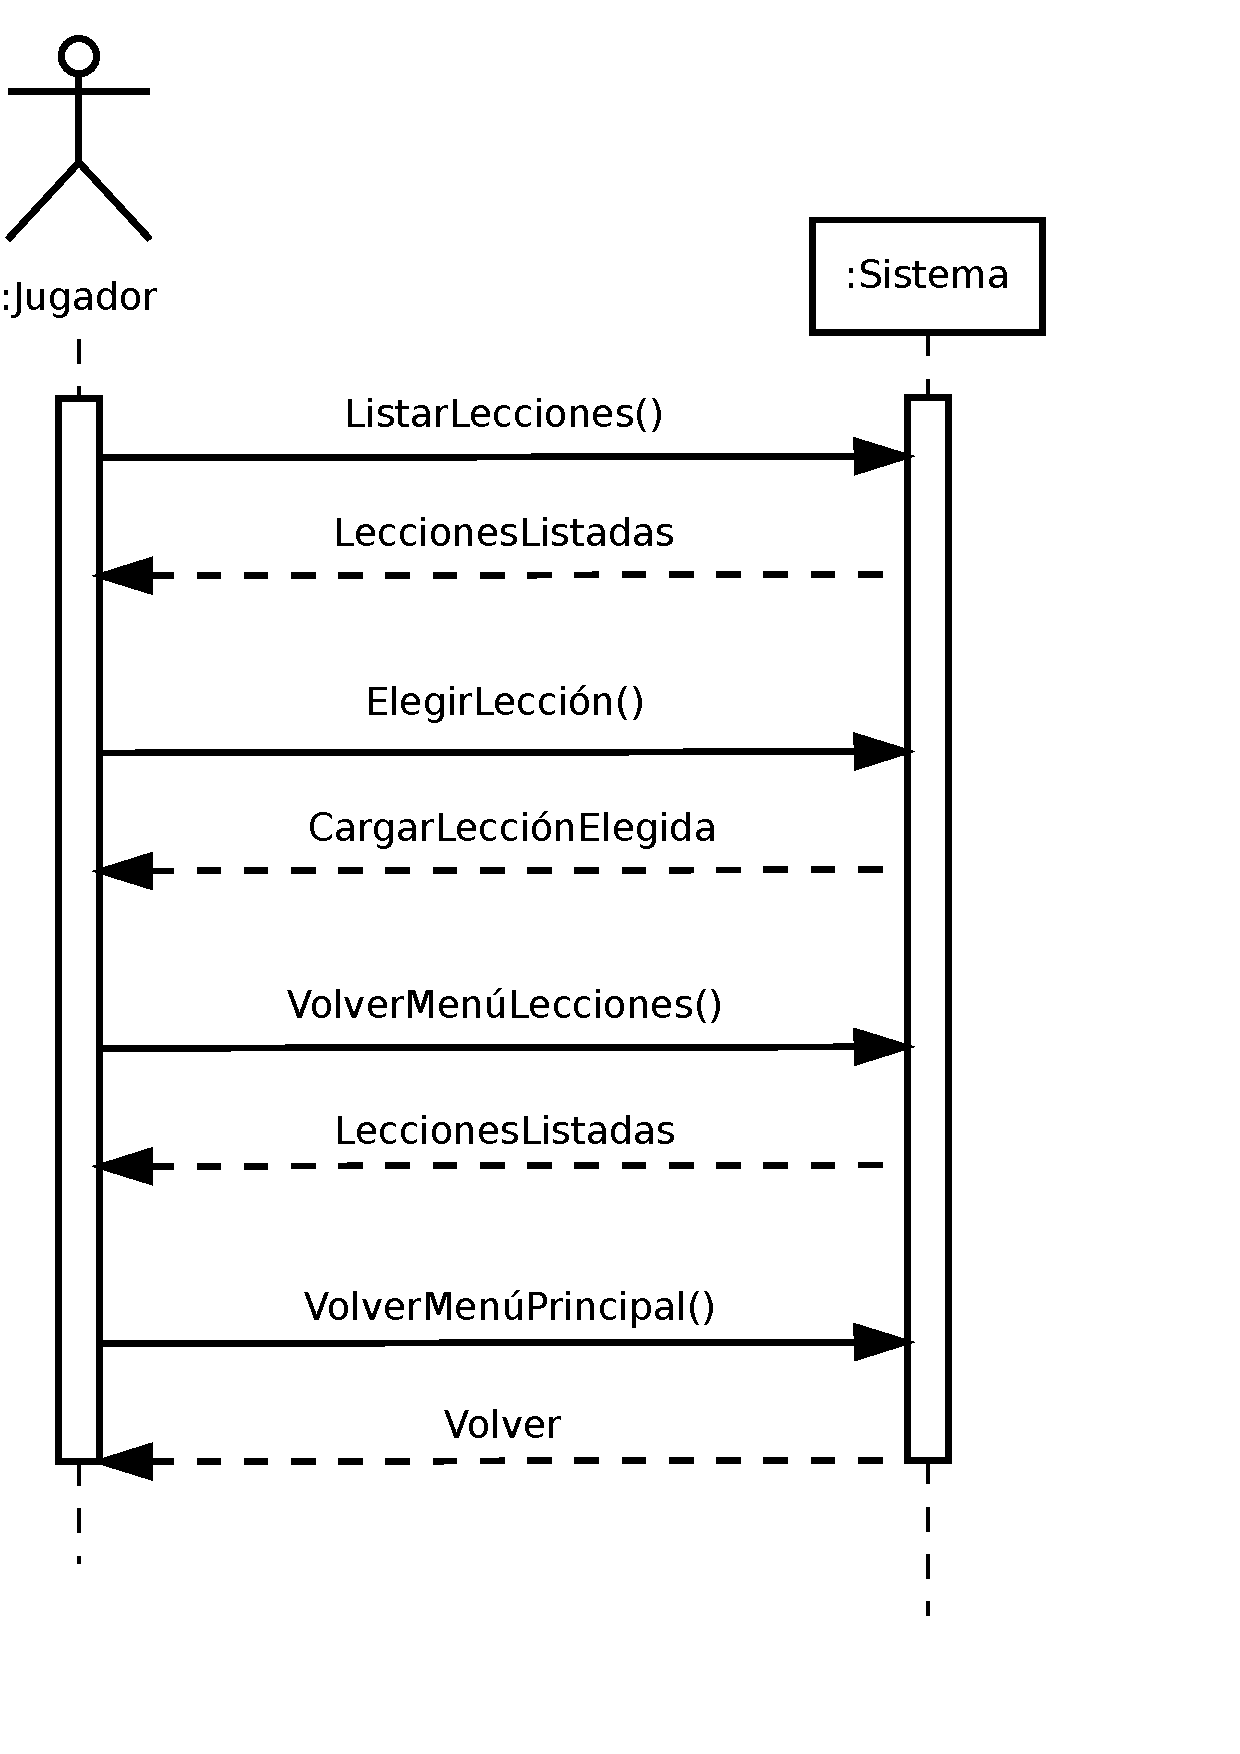
\includegraphics[trim=0cm 4cm 0cm 0cm, clip=true, width=0.5\textwidth]{4_analisis/diagsec_caso7_esc1}
  \caption{Diagrama de secuencia, selección delecciones, escenario principal}
\end{figure}


\begin{description}
\item[Operación] ListarLecciones()
\item[Actores] \jugador\, \sistema\
\item[Responsabilidades] Mostrar el menú de selección de lecciones y listar
  todas las lecciones disponibles.
\item[Precondiciones] El usuario eligió la opción \textit{Lecciones} en el menú
  principal.
\item[Postcondiciones] $\quad$
  \begin{itemize}
  \item Se muestra la interfaz del menú de selección de lecciones.
  \item Se listan las lecciones cargadas en el sistema
  \end{itemize}
\end{description}

\begin{description}
\item[Operación] ElegirLección()
\item[Actores] \jugador\, \sistema\
\item[Responsabilidades] Cargar y mostrar la lección elegida por el usuario.
\item[Precondiciones] El menú de selección de lecciones está cargado y el
  usuario ha elegido una de las lecciones.
\item[Postcondiciones]$\quad$
  \begin{itemize}
  \item Se oculta el menú de selección de lecciones.
  \item Se interpreta el fichero de lección elegido.
  \item Se muestran los elementos multimedia pertenecientes a la lección
    elegida.
  \end{itemize}
\end{description}

\begin{description}
\item[Operación] VolverMenuLecciones()
\item[Actores] \jugador\, \sistema\
\item[Responsabilidades] Descargar la lección actual y volver al menú anterior.
\item[Precondiciones] $\quad$
  \begin{itemize}
  \item El usuario ha terminado de ver la lección elegida.
  \item El usuario ha pulsado la tecla \texttt{escape} o el botón \textit{volver}.
  \end{itemize}
\item[Postcondiciones] $\quad$
  \begin{itemize}
  \item Se descarga la lección actual.
  \item Se muestra de nuevo el menú de selección de lecciones.
  \end{itemize}
\end{description}

\begin{description}
\item[Operación] VolverMenuPrincipal()
\item[Actores] \jugador\, \sistema\
\item[Responsabilidades] Descargar el menú de selección de lecciones y volver al
  menú principal.
\item[Precondiciones] El usuario ha pulsado la tecla \texttt{escape} o el botón \textit{volver}.
\item[Postcondiciones] $\quad$
  \begin{itemize}
  \item Se descarga el menú de selección de lecciones.
  \item Se carga y muestra el menú principal
  \end{itemize}
\end{description}

\subsubsection{Escenario alternativo}
\begin{figure}[h!]
  \centering
  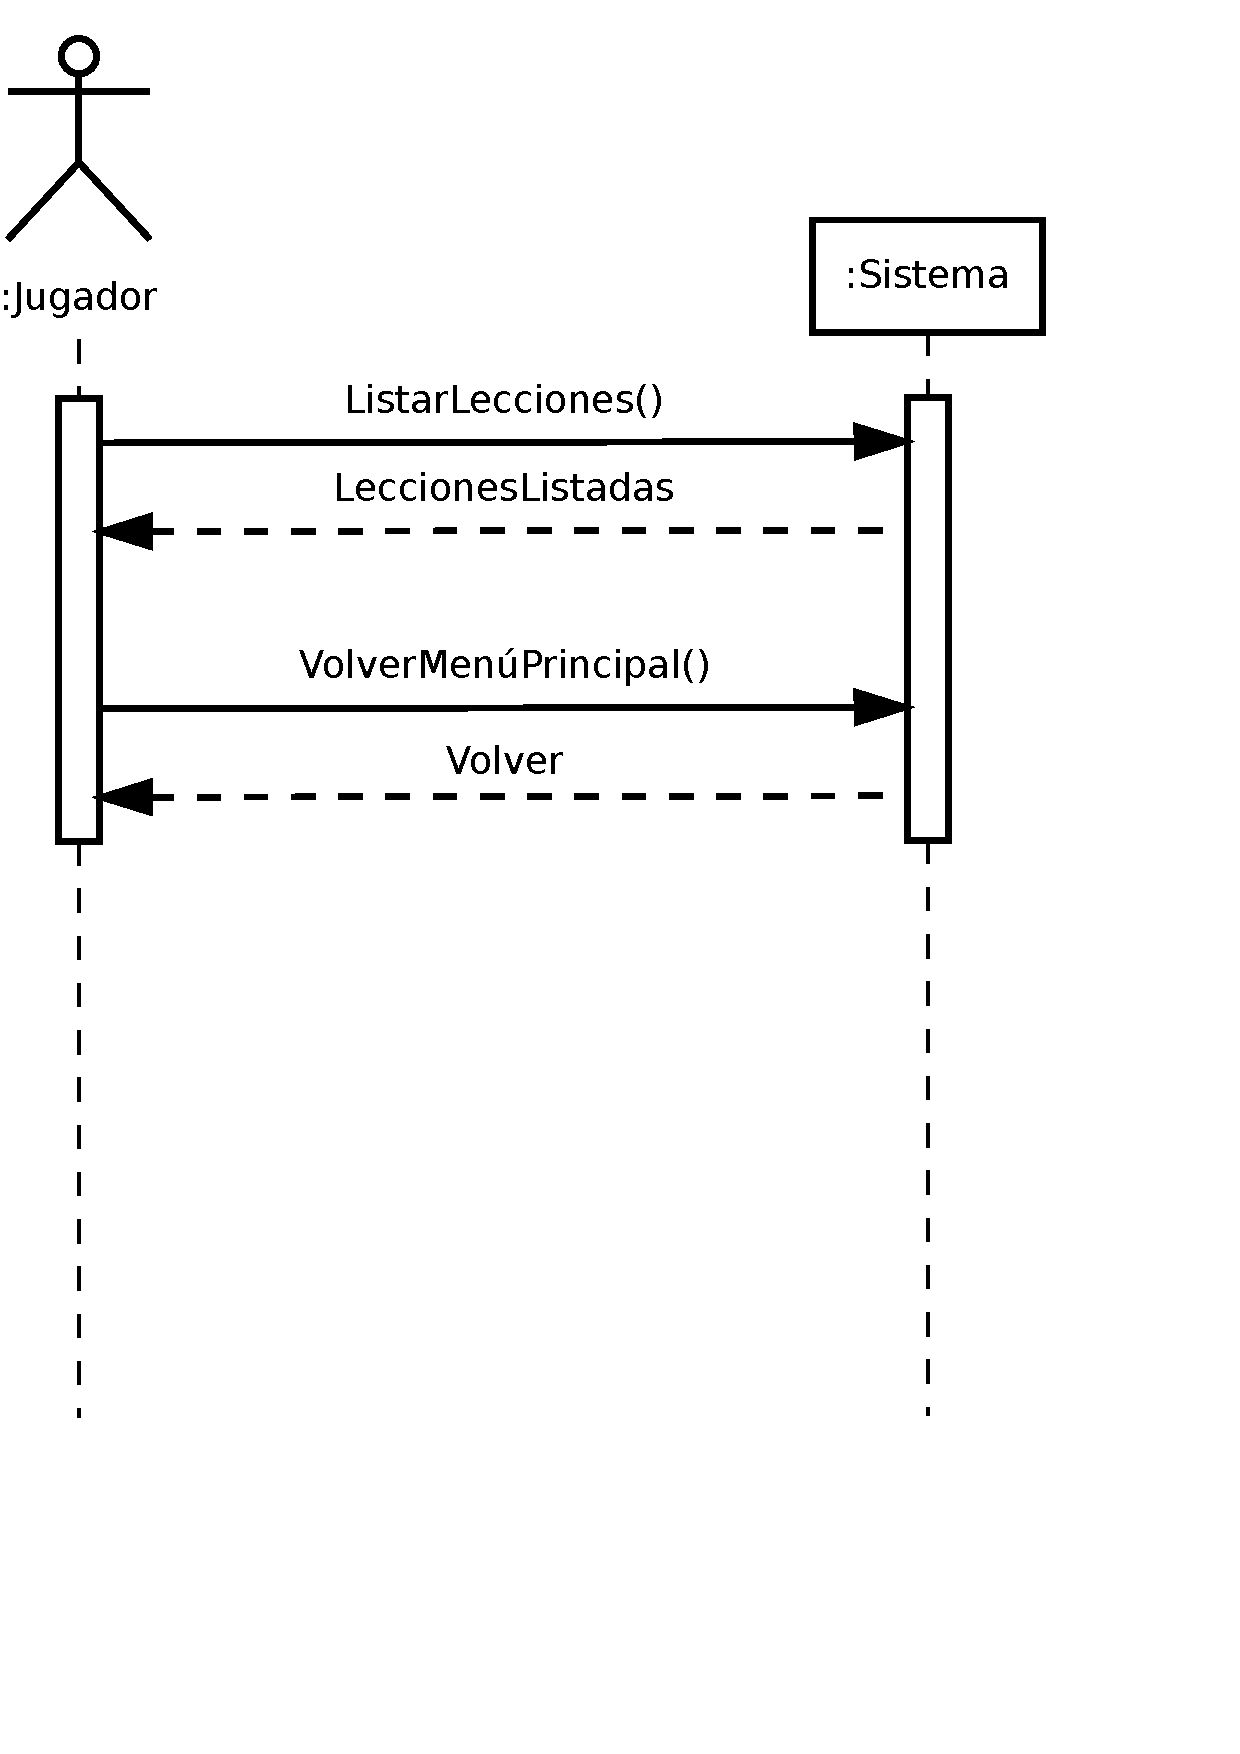
\includegraphics[trim=0cm 12cm 0cm 0cm, clip=true, width=0.5\textwidth]{4_analisis/diagsec_caso7_esc2}
  \caption{Diagrama de secuencia, selección de lecciones, escenario alternativo}
\end{figure}

\begin{description}
\item[Operación] ListarLecciones()
\item[Actores] \jugador\, \sistema\
\item[Responsabilidades] Mostrar el menú de selección de lecciones y listar
  todas las lecciones disponibles.
\item[Precondiciones] El usuario eligió la opción \textit{Lecciones} en el menú
  principal.
\item[Postcondiciones] $\quad$
  \begin{itemize}
  \item Se muestra la interfaz del menú de selección de lecciones.
  \item Se listan las lecciones cargadas en el sistema
  \end{itemize}
\end{description}

\begin{description}
\item[Operación] VolverMenuPrincipal()
\item[Actores] \jugador\, \sistema\
\item[Responsabilidades] Descargar el menú de selección de lecciones y volver al
  menú principal.
\item[Precondiciones] El usuario ha pulsado la tecla \texttt{escape} o el botón \textit{volver}.
\item[Postcondiciones] $\quad$
  \begin{itemize}
  \item Se descarga el menú de selección de lecciones.
  \item Se carga y muestra el menú principal
  \end{itemize}
\end{description}

%%% Local Variables: 
%%% mode: latex
%%% TeX-master: "../memoria"
%%% End: 

%%% Local Variables: 
%%% mode: latex
%%% TeX-master: "../memoria"
%%% End: 


\chapter{Diseño}
\label{chap:diseno}
%En este capítulo se presentarán los detalles de diseño del proyecto, basándonos
en el análisis mostrado en el capítulo anterior. El modelo de clases de diseño
representado aquí es más fiel a la implementación final que el diagrama de
clases conceptuales, pero aún así hay detalles que no se han contemplado por ser
demasiado cercanos a los detalles de implementación.

También en el presente capítulo se detallarán las decisiones de diseño en
relación al aspecto visual de la aplicación, extendiéndonos en el proceso de
creación del logotipo del juego así como de la interfaz gráfica de usuario.

\section{Diagrama de clases de diseño}

Tras la fase de diseño, componían el sistema más de 40 clases, por lo que hemos
tenido que dividir los diagramas en varias partes, intentando seguir cierto
criterio a la hora de elegir qué clases formarán parte de cada división.

En todos los diagramas aparecen, en aras de mantener el contexto, las clases
básicas de la aplicación: \textit{Juego} y \textit{Estado}. Además, hay algunas
otras clases que también se repetirán entre diagramas por conveniencia. Para
mantener la legibilidad, se han ocultado los miembros privados y protegidos.

\begin{itemize}
\item En el primer diagrama (figura~\ref{fig:diagrama_clases_1}) aparecen las clases
  relacionadas con el \textit{menú principal}, clases de utilidades (logging y
  animación), y clases para representar elementos gráficos.
\item En el segundo diagrama (figura~\ref{fig:diagrama_clases_2}) aparecen las
  clases relacionadas con el subsistema de análisis del audio, así como las
  secciones \textit{Analizador de Notas} y \textit{Calibrar micrófono}.
\item En el tercer diagrama (figura~\ref{fig:diagrama_clases_3}) aparecen todas las
  clases relacionadas con la sección de \textit{Canciones}.
\item En el cuarto y último diagrama (figura~\ref{fig:diagrama_clases_4}) aparecen
  las clases relacionadas con el motor de \textit{lecciones}.
\end{itemize}

\begin{figure}[htp!]
  \centering
  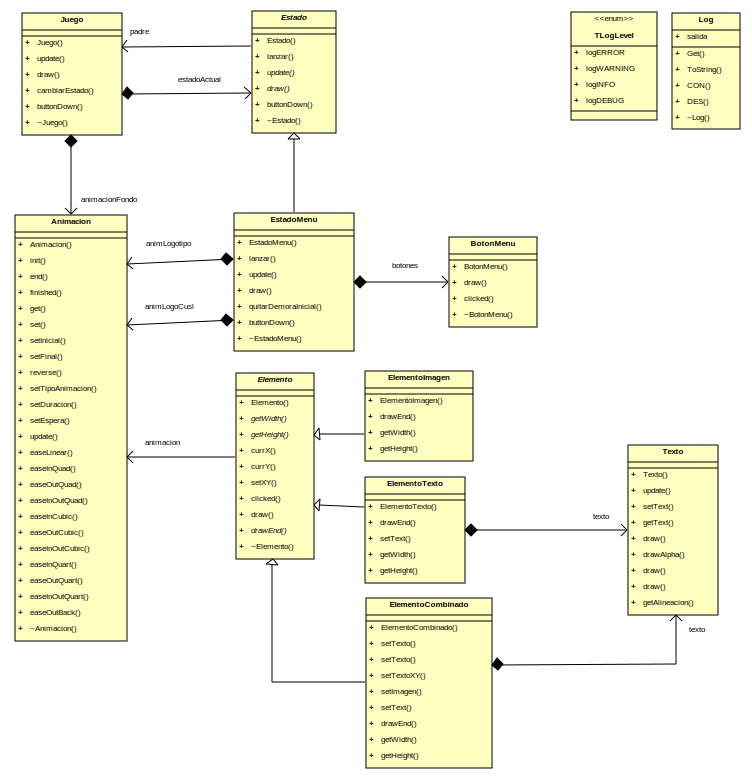
\includegraphics[width=\textwidth]{5_diseno/diagrama1}
  \caption{Diagrama de clases de diseño, parte I}
  \label{fig:diagrama_clases_1}
\end{figure}

\begin{figure}[htp!]
  \centering
  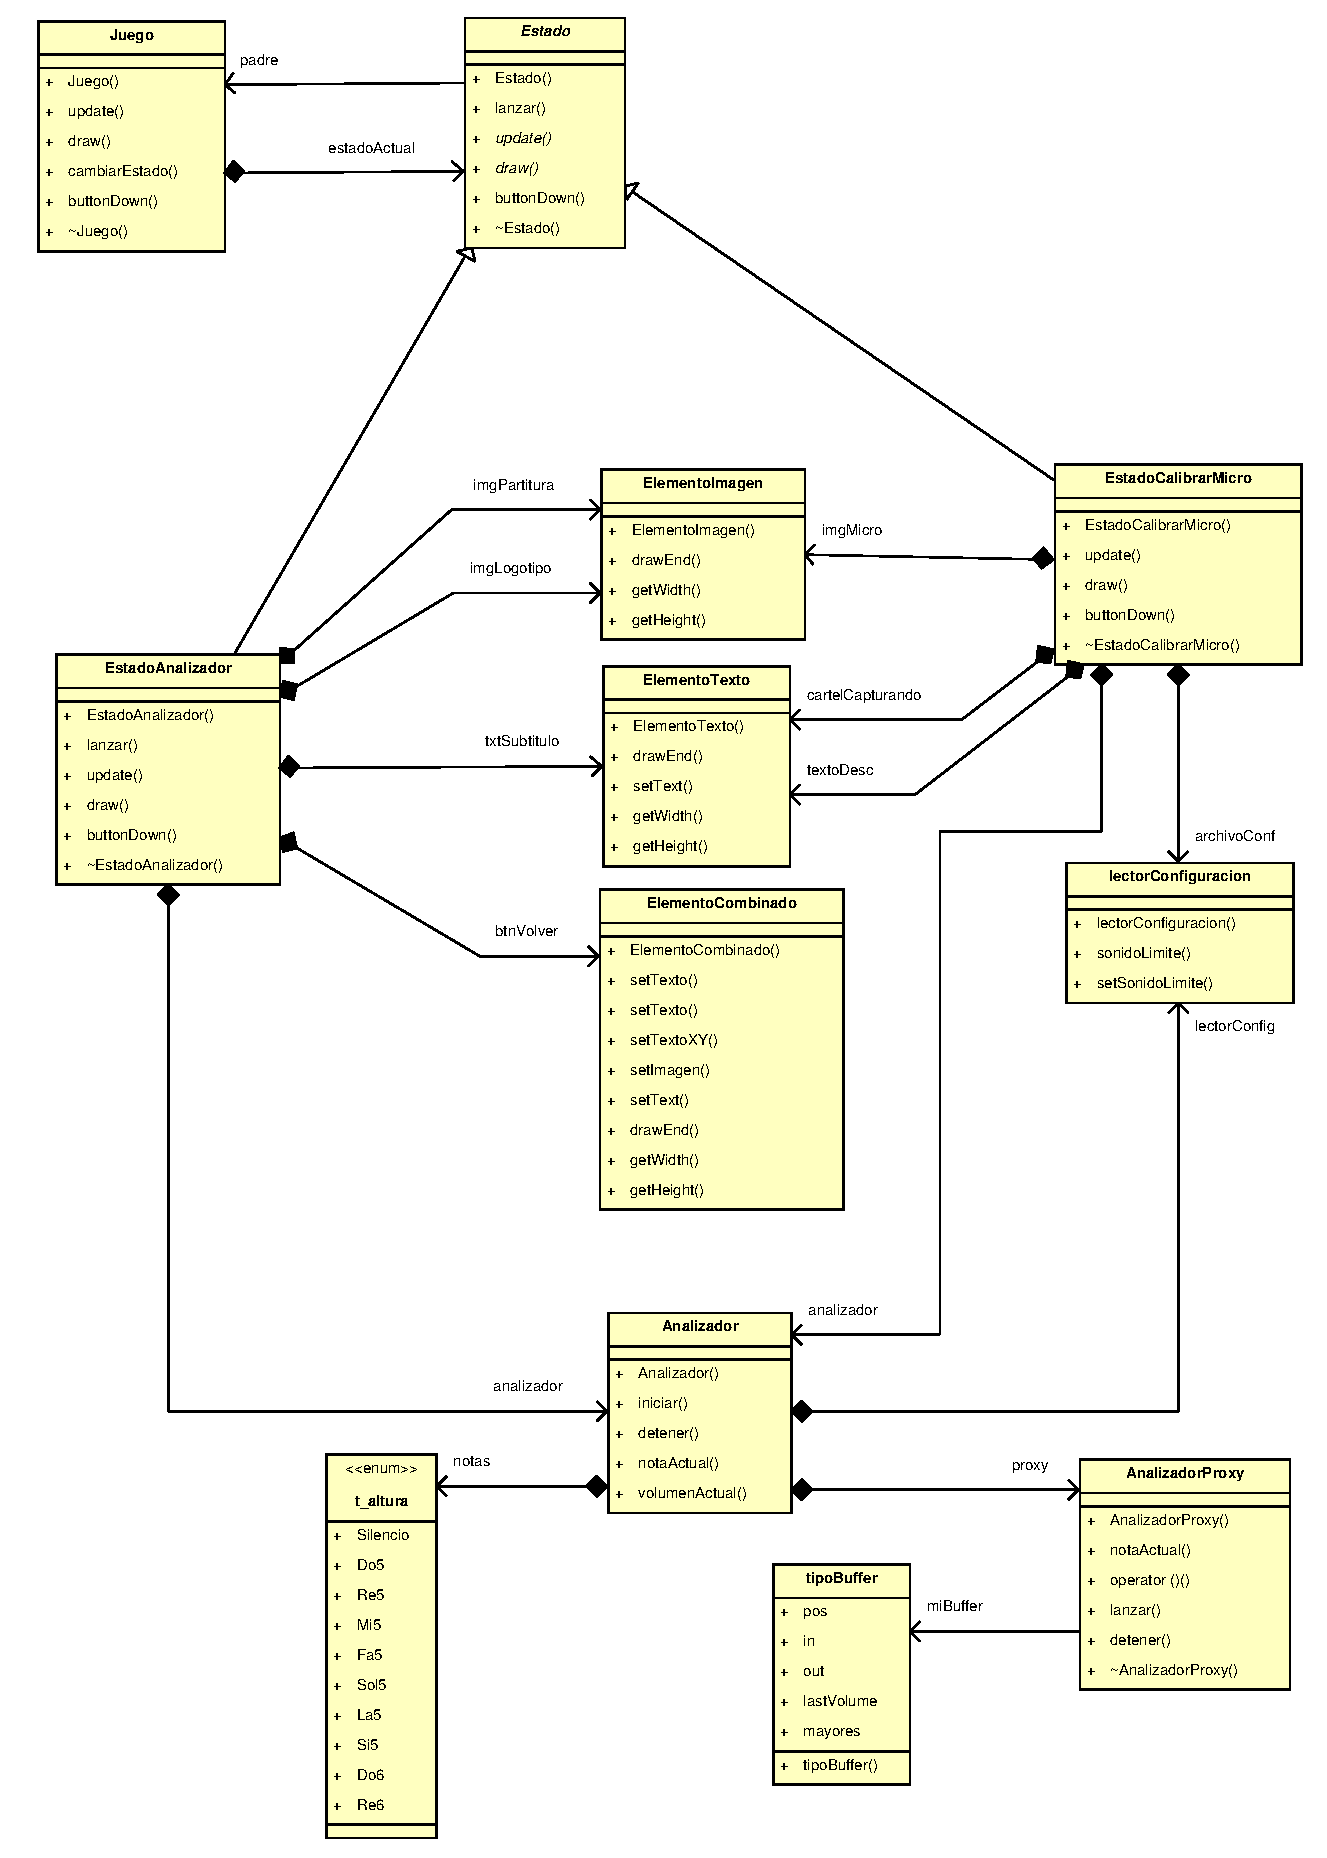
\includegraphics[width=\textwidth, clip=true, trim=0cm 0cm 0cm 0cm]{5_diseno/diagrama2}
  \caption{Diagrama de clases de diseño, parte II}
  \label{fig:diagrama_clases_2}
\end{figure}

\begin{figure}[htp!]
  \centering
  \includegraphics[width=\textwidth, clip=true, trim=0cm 0cm 0cm 0cm]{5_diseno/diagrama3}
  \caption{Diagrama de clases de diseño, parte III}
  \label{fig:diagrama_clases_3}
\end{figure}

\begin{figure}[htp!]
  \centering
  \includegraphics[width=\textwidth, clip=true, trim=0cm 0cm 0cm 0cm]{5_diseno/diagrama4}
  \caption{Diagrama de clases de diseño, parte IV}
  \label{fig:diagrama_clases_4}
\end{figure}

\section{Diseño visual}
Teniendo muy presente que el público objetivo de \textbf{oFlute} es joven y
dinámico, el diseño visual del proyecto intentó adaptarse a lo que la audiencia
podría considerar más atractivo. Desde el inicio se fijaron ciertas premisas o
\textit{guías de branding} para oFlute, que se siguieron a rajatabla a la hora
de diseñar cada uno de los elementos.

\textbf{Interfaces limpias y minimalistas}. Era imprescindible que las
interfaces gráficas de cada una de las secciones tuviera un diseño limpio y
cuidado, manteniendo en el mínimo la cantidad de elementos a mostrar en pantalla
sin descuidar el diseño.

Para conseguirlo, se optó por utilizar un fondo blanco con un sutil patrón gris
claro, que se mantiene a lo largo de todas las secciones. Un gran ejemplo de esto
es la imagen de los títulos de crédito del juego.

\begin{figure}[htp!]
  \centering
  \includegraphics[width=0.7\textwidth]{apendice_manual_usuario/imagen_estadoIntro}
  \caption{Imagen de títulos de crédito de oFlute}
\end{figure}

\textbf{Paleta de colores pastel}. Para acompañar al blanco limpio de los
fondos de la interfaz se ideó una paleta de colores amplia, basado en tonos
brillantes, cercanos a pastel. Esta paleta está presente tanto en el logotipo de
oFlute, como en el resto de secciones. En especial, el menú principal se
benefició enormemente del uso de esta paleta de colores en los botones de las
secciones.

\begin{figure}[htp!]
  \centering
  \includegraphics[width=0.8\textwidth]{5_diseno/imagen_escala_colores}
  \caption{Detalle de la paleta de colores de oFlute}
\end{figure}

\textbf{Logotipo}. A la hora de diseñar el logtipo, se hizo un
\textit{brainstorming} inicial en busca de conceptos relacionados con el
proyecto: notas musicales, flautas, pentagramas, claves de sol, etcétera.

Finalmente, decidimos utilizar el concepto de la flauta a través del espacio
negativo que genera dibujar solo los orificios de la misma, manteniendo el
tamaño original de los mismos.

\begin{figure}[htp!]
  \centering
  \includegraphics[width=\textwidth]{5_diseno/imagen_composite}
  \caption{Logotipo de oFlute original sobre blanco, sobre negro y en blanco y
    negro}
\end{figure}

\textbf{Tipografía}. Para adecuarse al diseño minimalista propuesto, se buscaron
tipografías simples y limpias. Para el logotipo se usó la fuente 232 MKSD
Round~\cite{fuentelogo}, y para los textos de la aplicación se usó la fuente
Miso~\cite{fuentetexto}.

%%% Local Variables: 
%%% mode: latex
%%% TeX-master: "../memoria"
%%% End: 


\chapter{Implementación}
\label{chap:implementacion}
%Un análisis claro y un diseño conciso no garantizan que, a la hora de
implementar el sistema planteado, no se encuentre ninguna dificultad o
imprevisto. Así pues, en este capítulo comentaremos los retos y detalles que más
relevancia o complejidad han presentado durante la fase de la implementación del
proyecto.

De igual modo, durante el desarrollo de la aplicación se mantuvo actualizada una
bitácora, accesible en línea~\cite{ofluteblog}, en la que se fueron detallando,
a medida que aparecían, muchas de estas dificultades.

Como complemento a la lectura de este capítulo se recomienda tener una copia
local del repositorio del proyecto, disponible para su libre descarga desde la
forja oficial~\cite{ofluteforja}. En él se encuentra todo el código fuente
original, así como la documentación en formato \textit{Doxygen}~\cite{doxygen}.

\section{Carga y uso de fuentes TrueType en Gosu}

Como se ha comentado previamente, \textbf{oFlute} hace uso de la biblioteca
\textit{Gosu}, que proporciona una API sencilla para el acceso al sistema
gráfico, entre otras características. Este framework funciona en sistemas
Windows, GNU/Linux y Mac OS, aunque dada la dificultad de conseguir la
compatibilidad con todos ellos, la calidad y el rendimiento es bastante
desigual de un sistema a otro.

Una de estas desigualdades se presentaba a la hora de \textbf{cargar fuentes}
para mostrar textos. En su versión para GNU/Linux, el módulo para el pintado de
textos de Gosu (que comprende la clase \texttt{Gosu::Font} y las funciones
\texttt{Gosu::drawText} y \texttt{Gosu::createText}) solo permitía
utilizar fuentes que estuvieran ya instaladas en el sistema de forma global, de
modo que era imposible adjuntar un fichero con una fuente en formato
\texttt{TrueType}~\cite{reftruetype} para su carga en el juego. 

La instalación de fuentes en sistemas GNU/Linux siempre ha sido una operación
engorrosa que ha requerido permisos de administrador. Esto, unido a que tanto en
Windows como en Mac OS la opción de cargar fuentes desde un fichero sí estaba
disponible, supuso un grave problema en el planteamiento del proyecto.

Inicialmente se investigaron las razones de esta limitación. Al ser un proyecto
libre y abierto, revisamos el código de Gosu, concretamente la implementación
de la clase \texttt{Gosu::Font} previamente citada, de la que dependían todas
las otras funciones relacionadas con fuentes.

Las conclusiones que se sacaron fueron que Gosu, bajo GNU/Linux, implementaba el
renderizado de fuentes mediante una biblioteca llamada Pango~\cite{Pango}, de
bastante bajo nivel, y que por diseño está limitada al uso de fuentes de
sistema, ya que se orienta a herramientas del sistema operativo, no a
aplicativos de terceros.

Así pues, era necesario buscar una alternativa. En numerosos proyectos
previos~\cite{robinson} se había utilizado la biblioteca
\textbf{SDL}~\cite{refsdl}, un framework multimedia muy utilizado en
aplicaciones de audio, vídeo y juegos. Uno de los subsistemas que proporciona
SDL es \textbf{SDL\_ttf}~\cite{refsdlttf}, una biblioteca para el renderizado de
fuentes basadas en ficheros \texttt{TrueType}. Esto, unido a que la propia SDL
ya era una dependencia de Gosu, propició que se iniciara la implementación de
una solución basada en este medio.

\subsection{Funcionamiento de \texttt{SDL\_ttf}}

Para comprender cómo se implementó la solución al problema citado, el primer
paso es entender cómo funciona la biblioteca \texttt{SDL\_ttf} para poder ver
cómo se corresponde luego con Gosu.

\subsubsection{Tipos de datos utilizados}

En común con el resto de módulos de SDL, SDL\_ttf se basa en un tipo de datos
conocido como \textit{superficies} (\texttt{SDL\_Surface}). Estas superficies
representan mapas de bits cargados en memoria, y se utilizan para guardar las
imágenes que se cargan de los ficheros, así como para representar otros destinos
gráficos intermedios, como la propia pantalla.

Para representar el color del texto que vamos a pintar, SDL\_ttf utiliza la
estructura \texttt{SDL\_Color}, que guardará los valores de color de 8 bits para
los tres canales de color primario (rojo, verde y azul).

Además, SDL\_ttf define un tipo de datos propio, de nombre \texttt{TTF\_Font}, que
representa una fuente cargada a partir de un fichero, con un tamaño determinado.

\subsubsection{Funciones utilizadas}

SDL\_ttf precisa de una \textbf{inicialización} previa, que se lleva a cabo mediante la
llamada a \texttt{TTF\_Init()}. Igualmente, liberaremos los recursos ocupados
mediante \texttt{TTF\_Quit()}.

Para \textbf{cargar la fuente} a partir de los ficheros TrueType (con extensión
\texttt{.ttf}), se utiliza la función \texttt{TTF\_OpenFont(const char * fichero,
  int tamaño)}. Esta función recibe una cadena con el nombre del fichero y el
tamaño de letra a utilizar, y devuelve un puntero al tipo \texttt{TTF\_Font}.

\begin{minted}{cpp}
  TTF_Font * fuente = TTF_OpenFont("fichero_fuente.ttf", 25);
\end{minted}

Una vez cargada la fuente de nuestro interés, tendremos que \textbf{generar una
  superficie} con el texto que queramos. Para ello, SDL\_ttf ofrece una gran
variedad de funciones, según el suavizado del texto y el tipo de caracteres que
estemos utilizando. En nuestro caso, queríamos que la superficie tuviera fondo
transparente, así como usar caracteres en UTF-8~\cite{refutf8}, por lo que la
función que se eligió fue 
\begin{minted}{cpp}
  SDL_Surface * TTF_RenderUTF8_Blended (TTF_Font * fuente,
                                        const char * texto,
                                        SDL_Color color);
\end{minted}

Esta función devolverá un puntero a una superficie que se integrará
(\textit{blends}) sobre cualquier imagen, al tener el fondo transparente.


\subsection{Representación de imágenes en Gosu}

Una vez conocidos los tipos de datos y funciones que ofrece SDL\_ttf, es
necesario conocer cuáles son los tipos de datos equivalentes en Gosu, de forma
que pueda haber una \textit{conversión} de un tipo a otro.

\subsubsection{Mapas de bits de bajo nivel: Gosu::Bitmap}
La clase \texttt{Gosu::Bitmap} representa, en Gosu, un mapa de bits de bajo
nivel. Éste no contará con aceleración por hardware ni podrá mostrarse en
pantalla, pero podremos acceder directamente a los datos de los píxeles y
trabajar con ellos.

\texttt{Gosu::Bitmap} nos servirá de paso intermedio entre la superficie de SDL y las
imágenes habituales de Gosu.

\subsubsection{Imágenes de uso común: Gosu::Image}
En Gosu las imágenes y assets gráficos se manejan habitualmente con la clase
\texttt{Gosu::Image}, que representa un contenedor de más alto nivel que
\texttt{Gosu::Bitmap}, además de estar optimizado y poder pintarse en pantalla.

Podremos crear un objeto de esta clase a partir de un \texttt{Gosu::Bitmap}, consiguiendo
finalmente un objeto \textit{pintable}.


\subsection{Implementación final}

Conocidas las representaciones internas de ambas bibliotecas, se implementó una
clase con una interfaz similar a \texttt{Gosu::Font}, de modo que la transición
pudiera ser lo más transparente posible, de nombre \texttt{CustomFont}.

En el constructor se inicializa (de forma única, mediante una variable estática)
el subsistema \texttt{SDL\_ttf} utilizando la llamada
\texttt{TTF\_Init()}. Después, se carga la fuente indicada por los parámetros
del constructor. En ambos casos, se comprueba que el procedimiento ha sido
correcto, lanzando una excepción en caso contrario.

\begin{minted}{cpp}
static int initResult = TTF_Init();
if (initResult < 0)
   throw std::runtime_error("Could not initialize SDL_TTF");

font = TTF_OpenFont(fontName, fontHeight);
if (!font)
   throw std::runtime_error("Could not open TTF file " + fontName);

\end{minted}

Seguidamente, en el método de pintado (\texttt{draw}) se genera la superficie
con el texto que se indique, pasando el contenido de los píxeles a un contenedor
\texttt{Gosu::Bitmap} y finalmente generando un objeto \texttt{Gosu::Image} a
partir del mismo.

\begin{minted}{cpp}
SDL_Surface * surf = TTF_RenderUTF8_Blended(font, text, color);
if (!surface)
   throw std::runtime_error("Could not generate the surface");

Gosu::Bitmap temp;
temp.resize(surf.width(), surf.height());
std::memcpy(temp.data(), surf.data(), temp.width() * temp.height() * 4);

Gosu::Image image (graphic_target, temp);
image.draw(x, y, z);
\end{minted}

\subsection{Mejora de rendimiento}
Con la implementación anterior, en cada fase de dibujado se tenía que repetir el
proceso completo, aún cuando el texto no cambiase. Esto suponía una pérdida de
rendimiento considerable, sobre todo a la hora de hacer el \textit{trasvase} de
píxeles de la superficie de \texttt{SDL} al mapa de bits de Gosu.

La solución que se utilizó se basó en las implementaciones previas de la clase
\texttt{Gosu::Font}. La idea principal es utilizar un búffer de imágenes para
cada uno de los glifos de la fuente, que se iría rellenando a medida que fuera
necesario pintar cada caracter. Posteriormente, se utilizarían las imágenes en
ese búffer para pintar el texto indicado.

Así, por ejemplo, si en primer lugar se pide pintar el texto \textit{``Score''},
se renderizarían los caracteres \textit{'S'}, \textit{'c'}, \textit{'o'},
\textit{'r'} y \textit{'e'}, y se añadirían al búffer mencionado. Si más tarde
se necesita pintar el texto \textit{``Scoreboard''}, solo sería necesario
renderizar los caracteres \textit{'b'}, \textit{'a'} y \textit{'d'}, ya que de
los otros ya tenemos la representación gráfica.

Con este proceso se reducen al mínimo las llamadas a las funciones de fuentes de
\texttt{SDL\_ttf}, que solo se ejecutarán una vez por caracter y tipografía.

\subsection{Recepción}

Una vez contamos con una implementación funcional de la clase, se presentó el
parche en el foro oficial de Gosu~\cite{foroGosu}. En poco tiempo, el
desarrollador principal verificó el código propuesto e hizo una adaptación al
propio código original de la clase \texttt{Gosu::Font} para añadir la
propuesta. 

Por ende, desde la versión 0.7.20, el \textit{parche} forma parte
oficial de Gosu, y así se hace indicar en el fichero \texttt{TextUnix.cpp} de la
distribución oficial:

\begin{minted}{cpp}
// [...]

// Used for custom TTF files
// Adapted from customFont class by Jose Tomas Tocino Garcia (TheOm3ga)
class SDLTTFRenderer : boost::noncopyable

// [...]
\end{minted}

Así pues, dado que la solución propuesta se integró en la distribución oficial,
nos deshicimos de la clase \texttt{customFont} a favor de la actualización de
\texttt{Gosu::Font}, dado que al fin y al cabo el funcionamiento interno es
el mismo.

\section{Animaciones dinámicas}
\label{sec:animaciones}

Una de las decisiones iniciales de diseño fue la de hacer la interfaz gráfica de
usuario lo más atractiva posible, intentando utilizar gráficos amigables y, en
la medida de lo posible, animaciones y efectos dinámicos.

Con esto, se tornaba necesario crear un sistema de animaciones lo más versátil
posible, de forma que dotar a los elementos de la interfaz de movimiento fuera
un proceso sencillo. 

\subsection{Antecedentes: animaciones en Flash}
Para evitar reinventar la rueda y tener una base estable con la que empezar, se
investigaron sistemas de animaciones ya existentes, evaluando diferentes
enfoques y aproximaciones, sobre todo en sistemas altamente relacionados con las
animaciones. En particular, nos centramos en Adobe Flash (\textit{anteriormente
  Macromedia Flash}) y la gran cantidad de código disponible relacionado con la
generación de animaciones dinámicas.

Especialmente interesante es el trabajo de Robert Penner, un programador
americano muy interesado en la programación matemática, que ideó un sistema de
animaciones dinámicas para ActionScript~\cite{actionscript} 1.0 y 2.0. Penner,
en su libro \textit{Programming Macromedia Flash MX}~\cite{libropenner} incluyó
un capítulo llamado \textit{Motion, Tweening and Easing} (que dada su
popularidad acabó ofreciendo de forma gratuita~\cite{capitulopenner}), en el que
por primera vez presentó y explicó con detalle su sistema de animaciones.

En el citado capítulo se desgranan las animaciones como ecuaciones dependientes
del tiempo y de las posiciones inicial y final, de forma que fuera fácil generar
una serie de funciones para determinar la posición de un objeto en cada
instante. Una vez presentados los conceptos iniciales, Penner desvela una serie
de ecuaciones de movimiento (que acabaron siendo bautizadas y mundialmente
conocidas como las \textit{Penner's Easing Equations}). Estas ecuaciones modelan
un gran número de movimientos, en función de cómo varía la posición respecto del
tiempo (y perceptualmente la aceleración/deceleración del objeto animado).

Además, por cada tipo de ecuación, Robert Penner generó tres tipos de
movimientos: de aceleración (\textit{ease in}), de deceleración o frenada
(\textit{ease out}), y de aceleración-deceleración (\textit{ease in-out}). Con
esto, quedaban cubiertas la práctica totalidad de los tipos de animaciones posibles.

Así, un ejemplo de ecuación podrían ser las cúbicas, que hacen que la posición
del movimiento se rija por una función cúbica del tiempo. Si graficamos la
relación del tiempo por la posición, ambos de 0 a 1, el resultado sería la
gráfica de la figura \ref{fig:ecuacion1}.

\begin{figure}[htp!]
  \centering
  \includegraphics[width=\textwidth]{6_implementacion/imagen_ecuacion1}
  \caption{Relación cúbica entre la posición y el tiempo}
  \label{fig:ecuacion1}
\end{figure}

Tras estudiar bien el código original, se decidió hacer una adaptación en C++,
de forma que se adaptara a las necesidades del proyecto.

\subsection{Adaptación en C++}
El primer paso fue portar las ecuaciones propiamente dichas -- esto es, las
funciones que generaban las posiciones intermedias. Dado que el lenguaje
original, ActionScript, es un derivado de EcmaScript~\cite{Ecmascript}, la
sintaxis es prácticamente idéntica a C++ en cuanto a asignaciones y operadores
se refiere, por lo que este paso fue prácticamente transparente.

Seguidamente, se ideó un \textit{wrapper} para estas ecuaciones, de forma que
fuera un objeto independiente el que se encargara de calcular las posiciones
intermedias de la animación, en lugar de tener que hacerlo los propios objetos
animados. Para ello, se creó la clase \texttt{Animación}, con las siguientes
características:
\begin{itemize}
\item Para cada instancia, permite animar un número arbitrario de valores, de
  forma que con un solo objeto \textit{Animacion} podamos animar la posición
  horizontal y vertical de un objeto, por ejemplo.
\item Permite elegir entre tres tipos de movimiento (\textit{ease in},
  \textit{ease out} y \textit{ease in-out}) para tres ecuaciones distintas
  (cuadrática, cúbica y cuártica), además de una ecuación especial con
  movimiento de ida y vuelta, y, lógicamente, movimiento uniforme. En total, 11
  posibles movimientos.
\item Capacidad para atrasar las animaciones, de forma que sea sencillo generar
  animaciones escalonadas de varios elementos sin tener que recurrir a
  \textit{callbacks}.
\end{itemize}

\subsection{Ejemplo de uso}

Supongamos que tenemos una pelota que queremos mover diagonalmente con un
movimiento de aceleración, desde la posición 0,0 hasta la posición 150, 300, en
30 pasos. Además, tenemos un cuadrado que habrá de moverse de la posición 0, 150
hasta la posición 150,150 cuando la pelota vaya por la mitad de su camino, y que
llegue a la vez que aquella.

Para cumplir este objetivo, crearemos dos objetos \texttt{Animación}, uno para
la pelota y otro para el cuadrado. En el caso de la pelota estaremos animando
dos parámetros, la posición horizontal y la vertical, y la duración será de 30
pasos. El tipo de movimiento será de aceleración, y la ecuación que elegiremos
será la cuadrática. Al no indicarse nada, no habrá espera inicial.

\begin{minted}{cpp}
// Creamos la instancia
Animacion animPelota (2, 30, Animacion::tEaseInQuad, 0);

// Asignamos la pos inicial y final de la coordenada horizontal
animPelota.set(0, 0, 150);  

// Coordenada vertical
animPelota.set(1, 0, 300);
\end{minted}

En el caso del cuadrado el movimiento sólo será horizontal, por lo que
animaremos un parámetro. Además, el movimiento comenzará cuando la anterior
animación vaya por la mitad (esto es, en el paso 15), y deberá llegar a la vez,
por lo que la duración será de 15 pasos.

\begin{minted}{cpp}
// Creamos la instancia de la clase
Animacion animCuadrado (1, 15, Animacion::tEaseInQuad, 15);

// Asignamos las posiciones inicial y final
animCuadrado.set(0, 0, 150);
\end{minted}

Una vez inicializados los objetos \texttt{Animación}, tendremos que hacer que,
en cada iteración del bucle de juego, las animaciones se actualicen. Para ello,
la clase \texttt{Animación} dispone de un método \texttt{update}. Además,
haremos uso del método \texttt{get} para obtener las posiciones intermedias y
así actualizar el objeto

\begin{minted}{cpp}
// ...
// En la fase update del bucle de juego
animPelota.update();
animCuadrado.update();

imagenPelota -> draw(animPelota.get(0), animPelota.get(1));
imagenCuadrado -> draw(animCuadrado.get(0), 150);
\end{minted}

Con esto, ya estará lista la animación de ambos objetos. De cualquier modo, la
clase \texttt{Animación} provee otros métodos que pueden resultar de interés,
como el método \texttt{finished}, que comprueba si las animaciones han
concluído. 

Además, las ecuaciones de los movimientos han sido implementadas en forma de
funciones estáticas, por lo que es posible acceder a las mismas para hacer
cálculos puntuales si fuera necesario. En tal caso, hay que tener en cuenta que
todas las ecuaciones reciben cuatro parámetros, estos son, en orden:

\begin{itemize}
\item Tiempo transcurrido.
\item Valor inicial del atributo a animar.
\item \textit{Delta} del atributo en la animación (final - inicial).
\item Duración de la animación en pasos.
\end{itemize}

Con esto, será posible controlar las animaciones de forma independiente, sin
necesidad de crear una instancia de la clase.


\section{Implementación del analizador básico}
\label{sec:implementacion_analizador}
Como se comentó en la planificación (ver \textit{\nameref{chap:calendario}}), la
viabilidad del proyecto dependía de conseguir una implementación temprana y
correcta del analizador de notas, pues es el núcleo de la aplicación y sin él,
ésta no tendría ningún sentido.

La implementación del analizador se dividió en dos partes. Por un lado, había
que iniciar la captura de audio, lanzando el subsistema de sonido y empezando a
capturar datos. Por otro lado, se tenía que hacer el análisis de los datos
leídos para determinar qué nota se estaba tocando.

\subsection{Lanzando el subsistema de audio}
A lo largo del proyecto se han utilizado distintas bibliotecas de sonido, aunque
en general la filosofía de todas era la misma, así que nos centraremos en los
detalles de la que finalmente se dio por definitiva, PulseAudio. Dentro de
PulseAudio, nos decantamos por la \textit{Simple API}~\cite{pulseaudiosimple},
que cubría todas las necesidades del proyecto sin añadir excesiva complejidad.

El principal concepto en una API de sonido de bajo o medio nivel es el
\textbf{flujo de sonido} o \textit{stream}. Los flujos pueden ser de entrada, de
salida o dúplex, y tienen una serie de características según las necesidades de
la aplicación. En PulseAudio, al tratarse de un servidor de sonido y no de una
simple biblioteca, exiten algunos parámetros necesarios más. Se utiliza la
función \texttt{pa\_simple\_new}, con bastantes parámetros, entre los que se
pueden encontrar:
\begin{description}
\item[Servidor] Normalmente será el servidor de sonido por defecto.
\item[Nombre del cliente y de flujo] Identifica la aplicación (\textit{oFlute})
  y el flujo (\textit{record}) frente al servidor de audio. Este nombre podrá
  verse, por ejemplo, en la aplicación de control de volumen
  (\texttt{pavucontrol}).
  \begin{figure}[ht!]
    \centering
    \includegraphics[width=0.7\textwidth]{6_implementacion/imagen_pavucontrol}
    \caption{Control de volumen, mostrando el cliente \textit{oFlute}}
  \end{figure}
\item[Tipo de flujo] En nuestro caso será de entrada, por lo que se utilizó la
  macro \texttt{\nohyphens{kPA\_STREAM\_RECORD}}.
\item[Tipo de \textit{sample}] Definirá el tipo de datos que se usará para
  representar los sonidos.
\item[Opciones de búffering] Según busquemos rendimiento, fiabilidad, poca
  latencia... tendremos que variar las opciones de búffering.
\end{description}

Una vez hayamos creado un flujo, que correrá en segundo plano, tendremos que
leer los datos que arroja. Para ello, la API simple de PulseAudio provee la
función \texttt{pa\_simple\_read}, que nos permitirá volcar en un búffer
temporal un fragmento de audio. La elección del \textbf{tamaño del búffer} es
otro de los valores que repercutirá enormemente en el rendimiento del sistema.

Finalmente, una vez hayamos terminado de leer datos, podremos liberar el flujo
utilizando \texttt{pa\_simple\_free}. Con esto, ya podremos abrir, leer y cerrar
el flujo de sonido del micrófono. 

La parte más compleja a la hora de tratar con flujos es la de elegir los
parámetros apropiados. Son muchísimos los valores que hay que configurar:
frecuencia de muestreo, tamaño del búffer, número de canales, longitud del
búffer intermedio, latencia deseada\ldots Si no sabemos exactamente en qué
influye cada uno, acabamos en un proceso de prueba y error que puede resultar
muy tedioso.

\subsection{Análisis del audio capturado}

La segunda parte del proceso consiste en procesar y analizar el audio capturado
en cada momento, de forma que podamos conocer qué nota se está tocando con la
flauta a través del micrófono.

Como se ha comentado previamente, el alma del procesamiento en este caso es la
aplicación de la \textbf{transformada rápida de Fourier}
(\ref{sec:fourier}). Esta herramienta será capaz de descomponer los fragmentos
de sonido en sus componentes de frecuencia. La biblioteca usada en este caso es
KissFFT~\cite{kissfft}, que da unos resultados muy buenos en cuanto a
rendimiento y precisión. 

En el caso que nos concierne, un procesamiento básico de la señal será
suficiente para poder discernir la nota, por lo que podremos trabajar con
transformadas de fourier reales (no complejas). Para ello, KissFFT ofrece
variantes de sus funciones, muy optimizadas.

El primer paso es inicializar la biblioteca. KissFFT es capaz de utilizar el
mismo búffer entre distintas iteraciones de un cálculo, por lo que ahorramos el
tiempo de guardar y liberar memoria. Esta inicialización se guarda en un objeto
de configuración.

\begin{minted}{cpp}
  kiss_fftr_cfg configFFT = kiss_fftr_alloc (BUFSIZE, 0, NULL, NULL);
\end{minted}

El siguiente paso será realizar el cálculo sobre el búffer de sonido.  La forma
en que el algoritmo FFT almacena sus resultados depende de dos parámetros
principalmente: la frecuencia de muestreo y el tamaño del búffer de entrada. En
el caso de la FFT real, KissFFT devuelve el espectro positivo, que contendrá
tantos valores (en forma de números complejos) como el búffer de entrada más
uno. Cada uno de estos elementos representará la intensidad (y fase) de una
componente de frecuencia en la muestra inicial.

Pero, ¿cómo asociamos cada componente a la frecuencia apropiada? Ahí es donde
entra la frecuencia de muestreo. En el vector que arroja el cálculo del FFT,
haremos una simple regla de tres: el primer elemento corresponderá a la menor
frecuencia (0Hz), y el mayor elemento a la mayor frecuencia audible (en nuestro
caso será 22050Hz, ya que la frecuencia de muestreo es de 44.1kHz, por el
teorema de Nyquist -- sección~\ref{sec:nyquist}).
$$
   \begin{array}{ccc}
       \textrm{Pos. final}  & \longrightarrow & 22050Hz\\
       \textrm{Pos. X} & \longrightarrow & \textrm{Frecuencia Y}
   \end{array}
$$

Una vez identificadas las frecuencias en el resultado de la operación, es
necesario computar la \textbf{magnitud} de cada una de ellas, hallando el módulo
del número complejo. Tras esto, la \textbf{frecuencia fundamental} (que
representará la nota que está tocando la flauta) \textit{debería} ser la que
mayor magnitud tenga.

\subsection{Acotando el resultado}
El siguiente paso fue analizar las frecuencias que proveía la flauta dulce para
las nueve notas que puede emitir utilizando técnicas básicas -- esto es, sin
contar las notas que se pueden emitir utilizando técnicas avanzadas, como tapar
a medias ciertos orificios. De este estudio se extrajeron los siguientes
resultados (tabla \ref{tab:frecuencias}).

\begin{table}[ht!]
  \centering
  \begin{tabular}[h]{|c|c|}
    \hline
    \textbf{Frecuencia aproximada} & \textbf{Nota} \\ \hline
    523.25 Hz & Do, octava 5\\ \hline
    592.163 Hz & Re, octava 5\\ \hline
    656.763 Hz & Mi, octava 5\\ \hline
    699.829 Hz & Fa, octava 5\\ \hline
    785.692 Hz & Sol, octava 5\\ \hline
    893.628 Hz & La, octava 5\\ \hline
    1001.29 Hz & Si, octava 5\\ \hline
    1076.66 Hz & Do, octava 6 \\ \hline
    1195.09 Hz & Re, octava 6 \\ \hline
  \end{tabular}
  \caption{Frecuencias aproximadas de las notas de la flauta dulce}
  \label{tab:frecuencias}
\end{table}

Redondeamos el rango de frecuencias a $[450, 1500]$, cualquier sonido fuera de
ese rango no se considera una nota válida. En el resto de casos, se compara la
frecuencia fundamental obtenida con los valores en la tabla, y se devuelve la
nota apropiada.

\subsection{Ejecución concurrente}

Uno de los problemas que se encontraron fue que, inicialmente, el proceso de
análisis se incluyó dentro de la fase de cálculo de la lógica dentro del
\textit{game loop}. El resultado fue bastante poco satisfactorio, ya que el
cálculo de la FFT ralentizaba mucho el hilo, que tenía que esperar a que
concluyera para seguir renderizando el siguiente fotograma.

Así, se decidió, como suele ser habitual en el desarrollo de videojuegos, mover
el control y análisis del audio a un hilo aparte. Para ello, se hizo uso de la
biblioteca de hilos de Boost, que resulta mucho más amigable y sencilla de usar
que otras alternativas como los \textit{POSIX Threads}. 

A nivel de implementación, el uso de hilos en Boost es muy sencillo. Es
necesario tener una clase con el operador de función -- esto es,
\texttt{operator()} -- sobrecargado. Creamos un objeto de esa clase y se lo
pasamos al constructor de \texttt{boost::thread}, que llamará al anteriormente
citado operador en una copia del objeto pasado.

\begin{minted}{cpp}
// Instancia de la clase
ClaseCallable objeto;

// Hilo, crea una copia de objeto y llama al operador ()
boost::thread hilo(objeto);

// [...]

// Esperamos a que termine el hilo
hilo.join();
\end{minted}

Uno de los problemas que rápidamente se encontraron fue que, al lanzar el hilo,
se hace una copia del objeto referenciado. Esto resultaba un problema, ya que el
analizador hace cierta inicialización previa, y al duplicarse el objeto ocurrían
problemas. El resultado fue utilizar \texttt{boost::ref}, que permite pasar
referencias por copia.

\begin{minted}{cpp}
// Hilo sobre el propio objeto, no se hace copia
boost::thread hilo(boost::ref(objeto));
\end{minted}

\section{Gestión de estados}
\label{sec:implementacion_estados}

La gestión de estados es uno de los retos principales a la hora de desarrollar
un videojuego. Es necesario contar un sistema de gestión de estados robusto, que
permita pasar de un estado a otro de forma sencilla, sin errores, y manteniendo
información entre transiciones si fuera necesario.

En el caso de \textbf{oFlute}, el gestor de estados no necesitaba funciones
avanzadas; las secciones son consecutivas, por lo que no hay necesidad de
incluir concurrencia. Así pues, se editó el gestor de estados en base a la clase
\texttt{Gosu::Window}. Esta clase modela, mediante métodos, las diferentes fases
del \textit{game loop}, a saber:
\begin{enumerate}
\item Gestión de la entrada del usuario, mediante los métodos
  \texttt{buttonDown} y \texttt{buttonUp}.
\item Procesamiento de la lógica, en el método \texttt{update}.
\item Dibujado de los gráficos, en el método \texttt{draw}.
\end{enumerate}

Así, se creó una clase \texttt{Estado} con los mismos métodos, y una clase
\texttt{Juego} (heredera de \texttt{Gosu::Window}), que sirviese de controlador
de estados. Inicialmente, el gestor tenía un método \texttt{cambiarEstado}, que
descargaba de memoria el estado actual y cargaba el siguiente. Durante un tiempo
funcionó bien, pero llegó un momento en que empezaron a aparecer fallos de
memoria difíciles de acotar.

Tras bastantes días de depuración, finalmente el problema se encontró en el
\textit{momento} en el que se hacía la carga y descarga de estados. El conflicto
surgía porque se hacían llamadas para cambiar de estado \textit{en cualquier
  momento}, ya fuera en la etapa de lógica, de dibujado, o de gestión de la
entrada. En el instante de la llamada, se descargaba el estado actual y se
cargaba el siguiente. Esto originaba que las tareas que se habían lanzado, como
por ejemplo las imágenes pendientes de dibujar, se ejecutasen sobre objetos que
habían sido reemplazados en memoria. A menudo las imágenes se encontraban en
búferes de Gosu y no había problema, pero una vez se integró el analizador de
notas, el sistema empezó a fallar.

\label{sec:resolucion_problema_estados}

La solución fue bastante trivial. Se creó un sistema con una pequeña cola de un
elemento en el gestor de estados (la clase \texttt{Juego}). En el momento en que
alguien quisiese cambiar de estado, se añadía a la cola el nuevo estado a
cargar, y se activaba una bandera. Tras completar esa iteración del \textit{game
  loop}, al principio de la siguiente se hacía la carga y descarga de estados.

Este sistema de gestión de estados se extendió para incluir estados concurrentes
(por ejemplo, para mostrar menús de pausa), y aunque no se incluyó en oFlute,
está prevista su integración en la próxima versión de Freegemas~\cite{freegemas}.

\section{Representación de canciones y lecciones}
El sistema de lecciones y el de canciones son los elementos que más dinamicidad
aportan a oFlute. El diseño e implementación de ambos dieron lugar a variadas
cuestiones de diseño. Una de las más importantes fue la forma de representar
lecciones y canciones en el sistema de ficheros.

Desde un principio se decidió que la representación de los ficheros de lecciones
y canciones debería ser sencilla y tener un formato cercano al usuario, para que
se pudiesen crear y modificar mediante el uso de un editor de texto plano.

El primer paso fue descartar por completo el uso de una estructura o notación
propia, ya que dificultaría el proceso de parseo, imposibilitando usar
bibliotecas de terceros para procesar los ficheros de entrada.

El siguiente paso fue comprobar las tecnología de representación más habituales
y utilizadas en el mercado. Se barajaron bastantes posibilidades, y finalmente
redujimos las posibilidades a dos opciones.

\subsubsection{JSON}
JSON (\textit{Javascript Object Notation}~\cite{JSON}) es un formato de
intercambio de datos muy sencillo y liviano, basado en un subconjunto de la
sintaxis de JavaScript. Hoy en día es el formato más utilizado en las
aplicaciones web, ya que el texto que representa la estructura es mínimo.

Se estructura en torno a dos elementos principales:
\begin{description}
\item[Pares] Formados por una clave o nombre, y un valor. Es la forma principal
  de representar un objeto o registro:
  \begin{minted}{javascript}
objeto = { nombre : "Pedro" };    
  \end{minted}
\item[Conjuntos] Que representan arreglos o vectores tradicionales. Lo habitual
  es que formen parte de un \textit{objeto}.
  \begin{minted}{javascript}
objeto = {coordenadas : ["norte", "sur", "este", "oeste"]};
  \end{minted}
\end{description}

Las ventajas de usar JSON son varias. Por un lado, el marcado necesario es
mínimo, por lo que el tamaño de los ficheros es muy reducido. Por otro, la
sintaxis es sencilla y se limita a las dos reglas anteriormente citadas.

\subsubsection{XML}
\label{sec:diseno_xml}
\acs{XML}~\cite{XMLSpec} son las siglas, en inglés, de \textit{eXtensible Markup
  Language} -- lenguaje de marcado extensible, un especificación para la
creación de documentos con marcas definidas por el usuario.

Utiliza una serie de \textit{etiquetas}, organizadas de forma jerárquica, que
siguen la forma \texttt{<nombre>}, donde \textit{nombre} es la identificación
del elemento que se está representando. Las etiquetas deben cerrarse utilizando
la sintaxis \texttt{</nombre>}. Entre las etiquetas de apertura y cierre pueden
anidarse otras etiquetas, así como información en formato texto.

\begin{minted}{xml}
<?xml version="1.0" ?>
<Documento>
  <Nombre>Nombre del documento</Nombre>
  <Autor>Autor del documento</Nombre>
  <Secciones>
    <Seccion>Lorem ipsum dillum</Seccion>
    <Seccion color_texto = "rojo">Sit amet, consectetuer</Seccion>
  </Secciones>
</Documento>  
\end{minted}

XML ofrece varias ventajas, desde el punto de vista de este proyecto, sobre JSON:
\begin{itemize}
\item Aunque la cantidad de texto necesario para marcar un documento es mayor
  que en el caso de JSON, las etiquetas de cierre aportan mayor legibilidad al
  documento, siendo más sencillo saber dónde termina cada bloque.
\item JSON solo permite introducir contenido como propiedades de objetos, usando
  el segundo elemento de los pares \textit{clave/valor}. En XML, es posible
  introducir contenido tanto dentro de las etiquetas como en forma de atributos
  de las mismas, de forma que con un mismo elemento podamos tener varias
  unidades de información.
\item XML es un lenguaje con más tiempo y uso que JSON, y las herramientas y el
  soporte existente es mucho más amplio. La inmensa mayoría de editores ofrecen
  resaltado de sintaxis para esta clase de ficheros, existen herramientas de
  validación XML, etcétera.
\end{itemize}

Por estas y otras razones, finalmente, se acabó eligiendo XML como medio de
representación de las lecciones y las canciones en oFlute.


%%% Local Variables: 
%%% mode: latex
%%% TeX-master: "../memoria"
%%% End: 


\chapter{Pruebas}
\label{chap:pruebas}
%En este capítulo se detallan las pruebas a las que se ha sometido
\textbf{oFlute}. Habitualmente, probar un videojuego o aplicación con gran
interactividad suele ser un proceso complejo. Dada la gran cantidad de
situaciones distintas que pueden tener lugar, es difícil recrear y probar todos
los escenarios posibles. Tanto es así que, en los grandes equipos de desarrollo,
hay empleados que se dedican al completo a probar los productos.

En oFlute, las pruebas se han organizado al final de cada iteración, comprobando
el correcto funcionamiento de cada nueva funcionalidad, por separado, y luego
integrando el conjunto. Además, ciertos módulos no asociados a iteraciones (como
el sistema de animaciones, sección \ref{sec:animaciones}) también fueron
probados de manera independiente.

\section{Pruebas unitarias}
Las \textbf{pruebas unitarias} se encargan de comprobar el correcto
funcionamiento de módulos y fragmentos por separado. En nuestro caso, todos los
módulos fueron probados de forma independiente, utilizando a tal efecto ramas de
desarrollo alternativas (\textit{branches}), antes de integrarlos en la rama de
desarrollo principal.

Mención especial merecen las pruebas unitarias relacionadas con el analizador
básico de notas, en la segunda iteración del proyecto. Tal y como se comentó en
la sección \ref{sec:implementacion_analizador}, al no tener experiencia previa
se tuvieron que hacer bastantes pruebas con el código relacionado con el control
del sonido para que el rendimiento fuera correcto y no apareciesen
problemas. Las pruebas unitarias en este módulo dieron lugar a decisiones de
cambios de bibliotecas en este módulo. Además, al ejecutarse en un hilo
separado, el código del analizador era propenso a generar fugas de memoria si no
se controlaban bien la vida y visibilidad de las variables utilizadas. 

\section{Pruebas de integración}
Según se comprobaban los módulos de manera individual, se iban integrando en la
rama de desarrollo principal, pasando a formar parte de la aplicación. Esta
integración también ha estado sujeta a pruebas, por un lado comprobando que los
módulos no cambiaban su comportamiento al ser integrados con el resto, y por
otro verificando que el funcionamiento general del sistema siguiera siendo
correcto.

Como se comentó en la sección \ref{sec:implementacion_estados}, uno de los
errores que más dificultad mostró, asociado a la gestión de estados, fue también
el más difícil de encontrar y reproducir. Gracias a las pruebas de integración y
al uso de herramientas de depuración, su resolución fue un éxito y sentó las
bases para un nuevo gestor de estados (sección
\ref{sec:resolucion_problema_estados}).

\section{Pruebas de jugabilidad}
Las \textbf{pruebas de jugabilidad} permitieron encontrar y rellenar lagunas en
el proyecto, haciendo que su uso fuera más sencillo para el usuario. En esta
etapa del proyecto se contó con la ayuda de usuarios reales inicialmente ajenos
al proyecto.

Entre las mejoras que surgieron a raíz de las pruebas de jugabilidad se
encuentra la implementación de la \textbf{barra de resaltado} (ver
\textit{\nameref{chap:manual_usuario}}), que aparece durante la interpretación
de las canciones para ayudar al usuario a conocer qué notas está tocando en cada
momento. Esto mejoró en gran medida las puntuaciones de los jugadores en las
partidas.

\section{Pruebas de interfaz}
Por último, una vez ajustada la jugabilidad y verificado que los módulos
funcionan bien de forma independiente y en integración, se dedicó un tiempo a
comprobar que la interfaz gráfica de usuario cumplía los requisitios mínimos que
se esperaban.

En particular, se hizo mucho hincapié en la duración de cada una de las
animaciones de cada sección. Animaciones largas podían llegar a ser tediosas,
mientras que unas animaciones cortas darían una desagradable sensación de
premura que no interesaba. Una vez ajustadas, se implementó la opción de poder
omitir las animaciones en pantalla, en cualquier sección y momento, mediante la
pulsación de la tecla \texttt{escape}. Esto permitiría que jugadores avanzados
pudieran llegar rápidamente a la sección de su interés de forma rápida.

Otra de las adiciones que surgieron tras las pruebas de interfaz fueron los
atajos de teclado. Se añadieron atajos para las opciones del menú principal, así
como el menú de selección de canciones y el de selección de lecciones. También
se habilitó la tecla \texttt{escape} para volver atrás en cualquier momento.

%%% Local Variables: 
%%% mode: latex
%%% TeX-master: "../memoria"
%%% End: 


\chapter{Conclusiones}
\label{chap:conclusiones}
%Durante el transcurso del desarrollo de oFlute, y sobre todo al término del
mismo, se han obtenido unas conclusiones y unos resultados, tanto de forma
personal como para con la comunidad, que intentaremos reflejar en este capítulo.


\section{Objetivos cumplidos}
Al término del desarrollo del proyecto, el proyecto ha completado todos los
objetivos a cumplir, presentes en el planteamiento inicial y detallados en la
sección \textit{\ref{sec:objetivos}}. En particular:

\begin{itemize}
\item Se llevó a cabo la creación del módulo de análisis de sonido, consiguiendo
  una efectividad en la detección de las notas muy alta.
\item Se hizo uso del módulo en una sección de análisis de notas y en el propio
  juego de interpretación de canciones, con resultados muy satisfactorios y
  funcionamiento correcto.
\item Además, el sistema de lecciones planteado se llevó a cabo correctamente,
  consiguiendo un motor dinámico bastante potente y fácilmente ampliable, con
  opción a añadir nuevas lecciones al sistema (apéndice
  \ref{chap:manual_lecciones}).
\item Finalmente, todos los objetivos se llevaron a cabo respetando la premisa
  de mantener una interfaz de usuario amigable y fluida, agradable a la vista y
  sencilla de usar.
\end{itemize}

\section{Conclusiones personales}

oFlute ha sido el proyecto más longevo al que me he enfrentado hasta ahora. A
pesar de tener conciencia de la envergadura del mismo desde el principio, el
tiempo para completarlo ha superado todas mis expectativas, sobre todo en lo que
a documentación se refiere. 

La causa de esto ha sido, en primer lugar, una planificación inicial algo
ineficiente y, por otro lado, mi recelo sobre los procedimientos actuales sobre
ingeniería del software. De cualquier modo, estoy bastante satisfecho con lo
obtenido, y esto me ha servido para aprender a regirme por una planificación de
forma más estricta.

\subsection{Conocimiento adquirido}

Gracias a oFlute he aprendido las técnicas básicas de la programación de audio,
sobre todo en la parte técnica más que teórica. Es esta parte teórica, sobre
todo la de análisis, la que me gustaría reforzar en un futuro, ahora que cuento
con las bases para conseguirlo. Como se comentó en el capítulo
\textit{\nameref{chap:fundamentos}}, los videojuegos relacionados con el audio
son un nicho aún poco explorado y que puede dar muchas satisfacciones, sobre
todo cuando el producto se orienta a un público joven.

Por otro lado, oFlute también me ha ayudado a aprender a usar bastantes
tecnologías auxiliares, en algunos casos meras herramientas que han facilitado
el trabajo y, en otros casos, elementos que resultaron ser de inestimable ayuda
e imprescindible uso al término del proyecto.

Una de estas tecnologías es \textbf{Boost}~\cite{boost}, un conjunto de
bibliotecas para C++ que amplían en gran medida la biblioteca estándar del
lenguaje. Un amplio número de componentes de Boost formarán parte del nuevo
estándar C++0x, por lo que me ha servido para ponerme al día en las
novedades que están por llegar.

\begin{figure}[htp!]
  \centering
  \includegraphics[width=0.4\textwidth]{8_conclusiones/imagen_logoboost}
  \caption{Logotipo de Boost}
\end{figure}

Utilizando como material de apoyo el libro \textit{``Beyond the C++ Standard
  Library''}~\cite{libroboost}, pude conocer una gran parte de las bibliotecas
de Boost, incluyendo punteros inteligentes, programación funcional, bibliotecas
para hilos, y utilizarlas en el proyecto.

Al tratarse de la principal biblioteca utilizada durante el desarrollo, oFlute
me ha provisto de un profundo conocimiento de \textbf{Gosu}~\cite{gosu},
permitiéndome implementar videojuegos con mucha más fluidez y labrándome un
pequeño \textit{framework} personal que utilizar de base en próximos
proyectos. 

\begin{figure}[htp!]
  \centering
  \includegraphics[width=0.4\textwidth]{8_conclusiones/imagen_logogosu}
  \caption{Logotipo de Gosu}
\end{figure}

Otra de las tecnologías que he aprendido ha sido \textbf{GNU Gettext}, que ha
servido para internacionalizar el proyecto. Aunque inicialmente se pensó en
utilizar una solución propia para la internacionalización el proyecto,
posteriormente se decidió usar esta tecnología, ampliamente conocida y
utilizada.

\section{Difusión y derivados}

A raíz del desarrollo de oFlute se abrieron varias vías de trabajo, en forma de
actividades de difusión de conocimiento, proyectos informáticos y participación
en comunidad.

\subsection{Conocimiento generado}

Además de servir como recurso para el correcto transcurso del proyecto, los
conocimientos adquiridos me permitieron, en numerosos casos, generar
documentación adicional e impartir talleres relacionados las tecnologías
previamente mencionadas.

En cuanto a Boost, se llevó a cabo un taller durante los \textit{Cursos de
  Verano de la OSLUCA}~\cite{cursosverano}, en el que se explicaron las partes
más importantes de esta colección de bibliotecas, con numerosos ejemplos de
muchas de ellas. Toda la documentación es libre~\cite{materialesCursoBoost}.

Por otro lado, impartí un taller~\cite{tallergosu} sobre la biblioteca Gosu en
colaboración con la ADVUCA~\cite{advuca}, cuya afluencia superó las 50
personas. Los materiales pueden descargarse
libremente~\cite{tallergosumateriales}.

Por último, tras la aplicación de GNU Gettext en oFlute, escribí una guía
concisa sobre traducción de proyectos con esta herramienta, que se puede
encontrar en el apéndice~\textit{\nameref{chap:tutorial_gettext}}.


\subsection{Freegemas}

Uno de estos proyectos \textit{``hijos''} de oFlute ha sido
\textbf{Freegemas}~\cite{freegemas}, un clon libre del popular juego tipo puzzle
\textit{Bejeweled}. Freegemas es multiplataforma, funciona tanto en GNU/Linux
como en Windows, y además forma parte oficial de Guadalinex~\cite{guadalinex},
por lo que es posible encontrarlo en los repositorios oficiales.

\begin{figure}[h!]
  \centering
  \includegraphics[width=0.55\textwidth]{8_conclusiones/imagen_freegemas}
  \caption{Logotipo de Freegemas}
\end{figure}

Además, Freegemas sirvió como base para una serie de tres artículos que
publiqué, junto al director del presente PFC, en la revista Linux
Magazine~\cite{linuxmagazine} sobre desarrollo de videojuegos en C++. Es posible
encontrar estos artículos en el archivo de la
revista~\cite{refarticulo1}~\cite{refarticulo2}~\cite{refarticulo3} bajo una
licencia Creative Commons.

\subsection{IV Concurso Universitario de Software Libre}

Por otro lado, gracias a oFlute tuve la oportunidad de participar en el IV
Concurso Universitario de Software Libre~\cite{cusl}. En el transcurso del
concurso formé parte de una comunidad muy unida, en la que reinó el apoyo y la
ayuda entre los concursantes. La final del concurso se celebró en la Escuela
Superior de Ingeniería de Cádiz, en la que oFlute obtuvo una mención
especial~\cite{cusl2}.

\begin{figure}[h!]
  \centering
  \includegraphics[width=0.65\textwidth]{8_conclusiones/imagen_logocusl}
  \caption{IV Concurso Universitario de Software Libre}
\end{figure}

Previa a la final nacional tuvo lugar la fase local del concurso, en el que el
proyecto también recibió un accésit al mejor proyecto de
innovación~\cite{cusllocal}.

%%% Local Variables: 
%%% mode: latex
%%% TeX-master: "../memoria"
%%% End: 


\appendix

\chapter{Herramientas utilizadas}
\label{chap:herramientas}
%En este primer apéndice se hará un repaso por las herramientas que han hecho
posible el desarrollo de oFlute, indicando qué tareas se han llevado a cabo con
cada una de ellas.

Dado que en la actualidad, la tendencia es la de mover la potencia de cálculo a
la \textit{nube}, también se mencionarán las herramientas \textit{online} que
han aportado al proyecto.

\section{Lenguajes y bibliotecas de programación}

\subsection{C++}
El lenguaje elegido para elaborar el proyecto fue \textbf{C++}. C++ es un
lenguaje de programación que extendió el lenguaje original C hacia el paradigma
de la orientación a objetos, mediante el uso de clases, y el paradigma de la
programación genérica, mediante plantillas, además de incluir muchas otras
novedades y facilidades.

Se decidió utilizar C++ por la familiaridad que teníamos con el mismo, así como
por la velocidad y optimización que se obtienen en comparación con otros
lenguajes, como Java.

\subsection{Gosu}
\textbf{Gosu}~\cite{gosu} es una biblioteca libre para el desarrollo de
videojuegos 2D para Ruby y C++. Entre sus características más atractivas se
encuentran la aceleración gráfica por hardware, la sencillez de su API,
completamente orientada a objetos, y su compatibilidad con sistemas GNU/Linux,
Windows y Mac OS.

Esta biblioteca, que está cerca de lanzar su versión 0.8, cuenta con una base de
usuarios cada vez mayor, en parte gracias a su relativa popularidad entre los
desarrolladores indie y en los eventos de programación rápida de videojuegos.

\subsection{PulseAudio}
\textbf{PulseAudio}~\cite{pulseaudio} (mencionado previamente en la sección
\ref{sec:pulseaudio1}) es un servidor de sonido multiplataforma, muy popular en
distribuciones GNU/Linux actuales. Se decidió su uso por lo intuitiva y sencilla
de utilizar que resultaba su API, así como su estabilidad, en comparaciones con
otras opciones previamente probadas.

\subsection{GNU Gettext}

\textbf{GNU Gettext}~\cite{refgettext} es un conjunto de herramientas de internacionalización de
proyectos muy sencilla y popular. Se utilizó porque es la solución más eficaz y
aceptada a la hora de traducir un proyecto. Se puede encontrar un manual
introductorio en el apéndice \textit{\nameref{chap:tutorial_gettext}}.

\subsection{KissFFT}
\textbf{KissFFT}~\cite{kissfft} es una biblioteca que implementa el algoritmo
FFT para el cálculo de transformadas rápidas de Fourier. Es una biblioteca
pequeña, razonablemente eficiente y portable, con capacidad para realizar
operaciones en distintos formatos.

Dado que el módulo de análisis de sonidos se basa en la transformada de Fourier,
era necesario encontrar una biblioteca que pudiera realizar el cálculo de forma
rápida y precisa. KissFFT resultó ser una candidata ideal para esta tarea.

\subsection{PugiXML}
\textbf{PugiXML}~\cite{pugixml} es una ligera biblioteca para el parseo y
procesamiento de ficheros XML. Tiene soporte completo Unicode, un parseador muy
veloz y capacidad para usar consultas XPath. Además, su implementación apenas
ocupa cuatro ficheros de trivial compilación, por lo que resulta muy sencillo
incluirla en cualquier proyecto.

Esta biblioteca se utilizó para el procesamiento de los ficheros de canciones y
lecciones, que utilizan XML para representar los distintos elementos.

\subsection{Boost}
\textbf{Boost}~\cite{boost} es un conjunto de bibliotecas para C++ para un gran
cantidad de situaciones distintas. Entre sus componentes se incluyen bibliotecas
para el procesamiento de textos, herramientas de gestión de memoria, expresiones
regulares, parseo de opciones de línea de comandos, adaptadores para
programación funcional y un largo etcétera.

Entre sus desarrolladores se encuentran muchos de los mejores programadores de
C++, y tal es su calidad y popularidad, que 10 de las bibliotecas que componen
Boost formarán parte del nuevo estándar de C++.

En oFlute se han utilizado bastantes partes de Boost: punteros inteligentes,
soporte para expresiones regulares, acceso al sistema de ficheros, y operaciones
con cadenas. Esto ha simplificado mucho el código, consiguiendo un estilo más
limpio y elegante, sin sacrificar funcionalidad alguna.

\section{Gestión de código}

\subsection{Subversion}
\textbf{Subversion}~\cite{refsubversion}, popularmente conocido como
\textbf{SVN}, es un sistema de control de versiones muy popular y
utilizado. Hasta hace unos años era el indiscutible ganador entre los sistemas
de control de versiones de código, y en la actualidad sigue siendo la opción
principal en muchas de las forjas de código más importantes de internet.

Se basa en un repositorio central, al que se envían los cambios de
los ficheros versionados. Además, a diferencia de otros sistemas como CVS, lleva
un control de revisiones a nivel global, no a nivel de fichero.

Subversion ha servido, en oFlute, sobre todo como backup online, además de
historial de cambios. En más de una ocasión ha sido necesario revertir los
cambios, y Subversion ha facilitado mucho el proceso, que en otras
circunstancias podría no haber sido posible.

\subsection{Forjas: RedIris y Google Code}
Para llevar un control del código del proyecto y servir como punto de encuentro
con otros usuarios y desarrolladores se abrió una forja para oFlute,
inicialmente dentro de la \textbf{Forja de Conocimiento Libre de la Comunidad
  RedIRIS}\footnote{\url{http://forja.rediris.es}}, gestionada por la Junta de
Andalucía. Esta forja ofrecía, además de un sistema de control de versiones del
código, una serie de herramientas para la gestión de bugs, emisión de noticias,
listas de correos, etcétera.

Desafortunadamente la forja de RedIris carecía de un mantenimiento adecuado, lo
que llevó al traspaso del proyecto a \textbf{Google Code}~\cite{ofluteforja}, un
repositorio de código ofrecido por Google mucho más actualizado y con un
mantenimiento adecuado. Una de los atractivos de Google Code es su sistema de
páginas wiki, que permite gestionar documentación online utilizando una sintaxis
sencilla y potente.

\subsection{Doxygen}
\textbf{Doxygen}~\cite{doxygen} es una herramienta de generación automática de
documentación de código fuente. Basándose en unos comentarios con una sintaxis
especial, Doxygen genera documentación en un gran número de formatos: HTML, PDF,
RTF, \LaTeX...

Esta herramienta se utilizó para generar toda la documentación del código del
proyecto en formato \ac{HTML}.


\section{Herramientas de diseño y diagramas}

\subsection{Adobe Photoshop}
\textbf{Adobe Photoshop}~\cite{photoshop} es la herramienta de edición gráfica de mapa de bits
más popular y utilizada en el mundo. Su longeva historia y profuso desarrollo ha
hecho que se convierta en la herramienta estándar a la hora de trabajar con
imágenes no vectoriales.

Aunque no se trata de una herramienta libre, se utilizó esta aplicación para la
creación de todo el apartado visual de oFlute. Todas las secciones fueron
diseñadas con esta herramienta, obteniendo un apartado gráfico atractivo y
minimalista.

\subsection{Inkscape}
\textbf{Inkscape}~\cite{inkscape} es una herramienta libre de edición de gráficos vectoriales. A
diferencia de Adobe Photoshop, Inkscape trabaja con formas definidas
matemáticamente, que es posible escalar y distorsionar sin causar pérdida de
datos. Esto hace que sea la herramienta perfecta para trabajar con logotipos y
diagramas.

Esta aplicación ayudó al diseño del logotipo oficial de oFlute, así como al
ajuste de ciertos diagramas pertenecientes a la documentación.

\subsection{Dia}
\textbf{Dia}~\cite{dia} es un editor de diagramas libre, parte de la suite ofimática de
GNOME. Tiene un diseño modular que le permite abordar una gran variedad de
diagramas distintos, desde diagramas de flujo hasta modelos entidad-relación,
UML, etcétera.

Este software se empleó para la generación de la mayor parte de los diagramas
presentes en esta memoria.

\subsection{BoUML}

\textbf{BOUML}~\cite{bouml} es una herramienta libre para diseñar diagramas siguiendo la
notación UML. Cuenta con utilidades de generación automática de código a partir
de diagramas en lenguajes C++, Java, PHP, Python e IDL. Es multiplataforma y
permite la generación de varios tipos de diagramas: diagramas de clases, de
interacción, de secuencia, de casos de uso, etc

\subsection{ImageMagick}

\textbf{ImageMagick}~\cite{imagemagick} es un conjunto de utilidades de línea de comandos para
mostrar, editar y convertir ficheros de imagen. Resultan especialmente útil a la
hora de procesar un gran número de imágenes de forma automática, como por
ejemplo cuando es necesario convertir varias imágenes de un formato a otro, o
cambiar el tamaño de numerosos ficheros.

\section{Edición de textos}

\subsection{GNU Emacs}
\textbf{GNU Emacs}~\cite{refemacs} es un potente editor multiplataforma. Su propio manual lo
describe como \textit{``un editor extensible, personalizable, auto-documentado y
  de tiempo real''}. Emacs es tan potente que a menudo los usuarios
experimentados no tienen que salir de su interfaz para realizar cualquier
operación, ya que desde el propio editor se puede, desde navegar por la red,
hasta revisar el correo electrónico.

Emacs ha sido el editor utilizado para escribir todo el código fuente del
proyecto, así como toda la documentación en \LaTeX. Sus diversos \textit{modos}
se ajustan a cada tipo de documento, proporcionando funciones que faciliten y
aceleren la edición de los textos.

\subsection{\LaTeX}
\textbf{\LaTeX}~\cite{latex} es un sistema de composición de textos, orientado especialmente
a la creación de libros, documentos científicos y técnicos que contengan
fórmulas matemáticas. Es muy utilizado para la composición de artículos
académicos, tesis y libros técnicos, dado que la calidad tipográfica de los
documentos realizados con LaTeX es comparable a la de una editorial científica
de primera línea.

La presente memoria ha sido escrita y maquetada con \LaTeX.

%%% Local Variables: 
%%% mode: latex
%%% TeX-master: "../memoria"
%%% End: 


\chapter{Manual de instalación}
\label{chap:manual_instalacion}
%A continuación se presentan las instrucciones de instalación de \textbf{oFlute}
en sistemas GNU/Linux basados en paquetería Debian~\cite{refdebian}, por
ser los que más auge están teniendo en la actualidad. Tomaremos como referencia
la distribución Ubuntu 10.10 Maverick~\cite{refubuntu}.

\section{Instalación de dependencias}

El primer paso a la hora de instalar oFlute es hacernos con las dependencias del
proyecto. Para ello, utilizaremos el gestor \texttt{apt-get}, pero para otros
sistemas el procedimiento será similar.

Primero, instalaremos las dependencias de la biblioteca Gosu:

\begin{minted}{bash}
  sudo apt-get install g++ libgl1-mesa-dev libpango1.0-dev \
  libopenal-dev libsndfile-dev libxdamage-dev libsdl-ttf2.0-dev \
  libboost-dev libfreeimage3 libfreeimage-dev
\end{minted}

Seguidamente, instalaremos el resto de dependencias:

\begin{minted}{bash}
  sudo apt-get install libboost-regex-dev libboost-filesystem-dev \ 
  libboost-thread-dev libpulse-dev
\end{minted}

\section{Descarga del código fuente}

El siguiente paso será hacernos con una copia local del repositorio, que
contiene el código fuente. Al tratarse de un proyecto libre, el repositorio es
de acceso público~\cite{ofluteforja}.

Haciendo uso del comando \texttt{svn}, haremos una copia local del repositorio
Subversion~\cite{refsubversion} en nuestro sistema con la siguiente orden:

\begin{minted}{bash}
  svn checkout http://oflute.googlecode.com/svn/trunk oflute
\end{minted}

Con ello, se creará una carpeta llamada \texttt{oflute} en la que se encontrarán
los ficheros de la rama principal (\texttt{trunk}) del proyecto.

\section{Compilación}

Como se ha comentado previamente, será necesario compilar la biblioteca Gosu
previamente. Para ello, se ha facilitado un objetivo en el script de compilación
\texttt{Makefile}~\cite{refmakefile} que automatiza el proceso.

Así, el primer paso será, estando en la carpeta recién creada, utilizar el
siguiente comando:

\begin{minted}{bash}
  make libgosu
\end{minted}

Una vez concluida la compilación de Gosu, pasaremos a compilar el propio
proyecto mediante la siguiente orden:

\begin{minted}{bash}
  make
\end{minted}

\section{Configuración del micrófono}
Antes de poder lanzar el juego, será necesario configurar las opciones de audio
del sistema operativo. Por defecto, la entrada de audio suele estar mutada, por
lo que será imposible que la aplicación tenga acceso al sonido proveniente del
micrófono.

Siguiendo con la referencia de Ubuntu, iremos al menú \textit{Sistema}, luego a
\textit{Preferencias} y, finalmente, elegiremos \textit{Sonido}. Una vez ahí,
pasaremos a la pestaña \textit{Entrada} y, en caso de que estuviera marcada,
desmarcaremos la opción \textit{Silenciar}, tal y como muestra la imagen.

\begin{figure}[h!]
  \centering
  \includegraphics[width=0.75\textwidth]{apendice_manual_instalacion/imagen_captura_1}
  \caption{Panel de configuración del micrófono}
\end{figure}

\vspace{-1cm}

\section{Ejecución}

Al término de las anteriores etapas, se habrá generado un ejecutable de nombre
\texttt{oflute}, por lo que será posible lanzar la aplicación a través del
siguiente comando:

\begin{minted}{bash}
  ./oflute
\end{minted}

%%% Local Variables: 
%%% mode: latex
%%% TeX-master: "../memoria"
%%% End: 


\chapter{Manual de usuario}
\label{chap:manual_usuario}
%En este capítulo se explicará el funcionamiento de la aplicación desde el punto
de vista del usuario final, detallando las opciones de cada una de las secciones.

Para poder acceder a la aplicación, tal y como se explicó en el apéndice 
\textit{\nameref{chap:manual_instalacion}}, será necesario utilizar el comando:

\begin{minted}{bash}
  ./oflute
\end{minted}

\section{Ejecución inicial}
Al lanzar la aplicación, se abrirá una ventana y aparecerán, consecutivamente,
la pantalla de créditos del autor y la pantalla de presentación del
juego. Pasados unos momentos éstas desaparecerán, aunque tiene la opción de
omitir cada una de las pantallas pulsando la tecla \texttt{escape}.

\begin{figure}[h!]
  \centering
  \includegraphics[width=0.8\textwidth]{apendice_manual_usuario/imagen_estadoAutor}
  \caption{Pantalla de créditos del autor}
  \vspace{-1cm}
\end{figure}

\begin{figure}[h!]
  \centering
  \includegraphics[width=0.8\textwidth]{apendice_manual_usuario/imagen_estadoIntro}
  \caption{Pantalla de presentación del juego}
  \vspace{-0.3cm}
\end{figure}

Una vez desaparezcan ambas pantallas, se iniciará una animación para mostrar el
menú principal. Puede cancelar la animación y mostrar rápidamente el menú
principal pulsando la tecla \texttt{escape}.

\begin{figure}[h!]
  \vspace{-0.1cm}
  \centering
  \includegraphics[width=0.8\textwidth]{apendice_manual_usuario/imagen_menuPrincipal}
  \caption{Pantalla del menú principal}
  \vspace{-1cm}
\end{figure}

Cuando las animaciones concluyan, el menú principal ya será completamente
funcional. Podremos acceder a las diferentes opciones, ya sea haciendo click con
el ratón en los botones de pantalla, o pulsando alguna de las teclas de acceso
directo. Las secciones y teclas asignadas son las siguientes:

\begin{itemize}
\item \textbf{Analizador de notas} (\textit{tecla 1}) Abre el analizador de
  notas.
\item \textbf{Canciones} (\textit{tecla 2}) Pasa al menú de selección de
  canciones.
\item \textbf{Lecciones} (\textit{tecla 3}) Abre el menú de elección de
  lecciones.
\item \textbf{Calibrar micrófono} (\textit{tecla 4}) Lanza el sistema de
  calibración del micrófono.
\item \textbf{Salir} (\textit{tecla 5}) Cierra la aplicación
\end{itemize}

Lo recomendado, en la primera ejecución de \textbf{oFlute}, es lanzar la sección
\textit{Calibrar micrófono}, ya sea pulsando el botón con el ratón o mediante la
tecla 4. Con esto nos cercioramos de que el programa es capaz de distinguir el
sonido del micrófono del ruido de fondo. Una vez hecho, ya estará todo listo
para acceder al resto de secciones.

\section{Sección -- calibrar micrófono}
Pulsando el botón correspondiente, o mediante la tecla 4, pasaremos a la sección
de calibración del micrófono. En primer lugar, aparecerá el siguiente mensaje:

\begin{figure}[h!]
  \vspace{-0.1cm}
  \centering
  \includegraphics[width=0.8\textwidth]{apendice_manual_usuario/imagen_seccionCalibrar1}
  \caption{Pantalla inicial de calibración del micrófono}
  \vspace{-1cm}
\end{figure}

Como se indica en el mensaje, para comenzar la calilbración el usuario deberá
pulsar la tecla \texttt{espacio} y guardar silencio en el micrófono durante dos
segundos. En ese momento, aparecerá el siguiente mensaje:

\begin{figure}[h!]
  \vspace{-0.1cm}
  \centering
  \includegraphics[width=0.8\textwidth]{apendice_manual_usuario/imagen_seccionCalibrar_mensaje1}
  \caption{Mensaje al inicio del calibrado}
\end{figure}

Una vez pasen los dos segundos y concluya la calibración, se mostrará el
siguiente mensaje:

\begin{figure}[h!]
  \vspace{-0.1cm}
  \centering
  \includegraphics[width=0.8\textwidth]{apendice_manual_usuario/imagen_seccionCalibrar_mensaje2}
  \caption{Mensaje al final del calibrado}
\end{figure}

Cuando concluya el proceso, la aplicación habrá guardado el valor umbral de
ruido del micrófono, lo que facilitará el análisis del sonido de la flauta.

Hay casos en los que la calibración será defectuosa, y un mensaje informará de
ello. En tal caso, no habrá más que comprobar la configuración del micrófono y
repetir el proceso de calibrado.

\section{Sección -- analizador de notas}

Al pulsar el botón correspondiente a la sección del analizador de notas,
mediante una animación aparecerán los elementos de esta parte de la aplicación
(figura \ref{fig:pantalla_analizador_notas} en página
\pageref{fig:pantalla_analizador_notas}).

\begin{figure}[h!]
  \vspace{-0.1cm}
  \centering
  \includegraphics[width=0.75\textwidth]{apendice_manual_usuario/imagen_seccionAnalizador}
  \caption{Pantalla del analizador de notas}
  \label{fig:pantalla_analizador_notas}
\end{figure}

Una vez terminen de mostrarse todos los elementos, el usuario podrá empezar a
utilizar la funcionalidad de la sección. En concreto, el analizador de notas nos
permite ver reflejada en el pentagrama la nota que toquemos con la flauta.

Su uso, pues, es muy sencillo. Simplemente tendremos que tocar nuestra flauta de
forma que el micrófono sea capaz de captar su sonido. Si lo hacemos
correctamente, el analizador mostrará en cada momento la nota que está tocando
sobre el pentagrama.

Una vez hayamos acabado de utilizar esta sección de la aplicación, podremos
pulsar en el botón \textit{Volver}, o en la tecla \texttt{escape} del teclado,
lo que nos llevará de vuelta al menú principal.

\section{Sección -- lecciones}
\vspace{-0.5cm}
Si seleccionamos la opción \textit{Lecciones} en el menú principal, o
alternativamente presionamos la tecla 3 del teclado, la aplicación mostrará una
animación para ocultar el menú principal y nos mostrará el menú de selección de
lecciones. 

\begin{figure}[h!]
  \vspace{-0.2cm}
  \centering
  \includegraphics[width=0.75\textwidth]{apendice_manual_usuario/imagen_seccionLecciones1}
  \caption{Pantalla del menú de selección de lecciones}
  \vspace{-1cm}
\end{figure}

\pagebreak

En cualquier momento podemos hacer click en el botón \textit{Volver al menú}, o
pulsar la tecla \texttt{escape} del teclado, para ir a la sección anterior.

En el menú de selección de lecciones podremos encontrar los siguientes
elementos:

\begin{itemize}
\item \textbf{Título} de la lección
\item \textbf{Descripción} de la lección
\item Botón \textbf{Comenzar lección}.
\item Botón \textbf{Anterior lección}.
\item Botón \textbf{Siguiente lección}.
\item Botón \textbf{Volver al menú}.
\end{itemize}

Mediante los botones de \textit{anterior} y \textit{siguiente lección} podremos
navegar entre las diferentes lecciones cargadas en el sistema. Haciendo uso de
los paneles de \textit{título} y \textit{descripción} nos informaremos sobre la
lección elegida. Una vez que tengamos claro la lección que queremos tomar,
pulsaremos en el botón \textit{comenzar lección.}

Una vez que decidamos comenzar la lección, el sistema ocultará los elementos del
menú de selección de lecciones mediante animaciones y, posteriormente, cargará y
mostrará los elementos de la lección elegida.

\begin{figure}[h!]
  \centering
  \includegraphics[width=0.8\textwidth]{apendice_manual_usuario/imagen_seccionLecciones2}
  \caption{Pantalla de lección de ejemplo}
\end{figure}

Las lecciones se muestran en forma de conjunto de elementos multimedia --
imágenes y texto -- de fácil comprensión, que el usuario podrá leer y estudiar
de forma independiente. En futuras versiones de la aplicación se podrán utilizar
lecciones de varias etapas, así como integrar sonidos y otro tipo de multimedia.

\section{Sección -- canciones}

El usuario podrá acceder a esta sección desde el menú principal, pulsando en la
botón \textit{Canciones}, o con la tecla 2 del teclado.

Al acceder, desaparecerá el menú principal y se mostrará el menú de selección de
canciones.

\begin{figure}[h!]
  \centering
  \includegraphics[width=0.8\textwidth]{apendice_manual_usuario/imagen_seccionCanciones1}
  \caption{Pantalla del menú de selección de canciones}
\end{figure}

Esta pantalla consta de los siguientes botones:
\begin{itemize}
\item \textbf{Anterior canción}, representado con una flecha hacia arriba.
\item \textbf{Siguiente canción}, representado con una flecha hacia abajo.
\item \textbf{Comenzar canción}, simbolizado con la palabra \textit{OK}.
\item \textbf{Volver}.
\end{itemize}

Mediante los botones \textit{anterior} y \textit{siguiente canción}, el usuario
podrá elegir el tema a interpretar con la flauta. Una vez esté resaltada la
canción correcta, el usuario deberá pulsar el botón \textit{Comenzar canción --
  OK} para que dé comienzo la interpretación.

También es posible pulsar el botón \textit{volver} para ir de nuevo al menú
principal.

\subsection{Interpretación de la canción}

Al lanzar la canción, aparecerá la pantalla de interpretación de canción, que
contiene numerosos elementos importantes para el jugador.

\begin{figure}[h!]
  \centering
  \includegraphics[width=0.8\textwidth]{apendice_manual_usuario/imagen_seccionCanciones2}
  \caption{Pantalla de interpretación de canción}
\end{figure}

\begin{enumerate}
\item \textbf{Marcador} de la puntuación del usuario.
\item \textbf{Pentagrama}. Sobre él aparecerán las notas.
\item \textbf{Notas}. Éstas irán apareciendo por el lado derecho del pentagrama,
  y moviéndose hacia la izquierda de forma ordenada y rítmica.
\item \textbf{Resaltado de nota}\label{barra_resaltado}. Resalta la posición en
  el pentagrama de la nota que está tocando el usuario con la flauta en cada
  momento. Esto ayuda visualmente a saber si estamos interpretando la nota
  correcta o no.
\item \textbf{Barra de interpretación}. Esta barra indica cuándo debe el usuario
  empezar a tocar la nota. 
\item \textbf{Barra de progreso}. Indica el progreso de la interpretación de la
  canción. Cuando la barra esté completa, la canción concluirá.
\end{enumerate}

La forma de juego es sencilla. Como se ha indicado, las notas aparecerán sobre
el pentagrama por el lado derecho, e irán desplazándose hacia la izquierda. Una
vez que una nota llegue a la \textit{barra de interpretación}, el jugador deberá
tocar con la flauta la nota correcta, de forma constante hasta que llegue el
turno de la siguiente nota.

Para ayudar al jugador, la barra de \textit{resaltado de nota} indicará en cada
momento qué nota se está tocandoo. Así, si en un instante es necesario tocar un
\textit{Sol} pero la barra de resaltado está por encima, el usuario sabrá que
debe cerrar más orificios de la flauta.

Las posibles \textbf{notas} que pueden aparecer son \textit{Do}, \textit{Re},
\textit{Mi}, \textit{Fa}, \textit{Sol}, \textit{La}, \textit{Si}, \textit{Do
  grave} y \textit{Re grave}. Las posibles figuras que podrán aparecer son las
siguientes:

\begin{description}
\item[Redonda] -- Dura cuatro tiempos.
\vspace{-0.1cm}
\begin{figure}[h!]
  \centering
  \includegraphics[width=0.05\textwidth]{apendice_manual_usuario/imagen_figRedonda}
  \caption{Figura musical -- Redonda}
\end{figure}

\vspace{-0.35cm}

\item[Blanca] -- Dura dos tiempos.
\vspace{-0.1cm}
\begin{figure}[h!]
  \centering
  \subfloat[Posición normal]{\parbox{0.5\textwidth}{\centering\includegraphics[width=1cm]{apendice_manual_usuario/imagen_figBlanca}}}
  \subfloat[Posición invertida]{\parbox{0.5\textwidth}{\centering\includegraphics[width=1cm]{apendice_manual_usuario/imagen_figBlancaInv}}}
  \caption{Figura musical -- Blanca}
\end{figure}

\vspace{-0.35cm}

\item[Negra] -- Dura un tiempo.
\vspace{-0.1cm}
\begin{figure}[h!]
  \centering
  \subfloat[Posición normal]{\parbox{0.5\textwidth}{\centering\includegraphics[width=1cm]{apendice_manual_usuario/imagen_figNegra}}}
  \subfloat[Posición invertida]{\parbox{0.5\textwidth}{\centering\includegraphics[width=1cm]{apendice_manual_usuario/imagen_figNegraInv}}}
  \caption{Figura musical -- Negra}
\end{figure}

\vspace{-0.35cm}

\item[Corchea] -- Dura la mitad que una negra.
\vspace{-0.1cm}
\begin{figure}[h!]
  \centering
  \subfloat[Posición normal]{\parbox{0.5\textwidth}{\centering\includegraphics[width=1cm]{apendice_manual_usuario/imagen_figCorchea}}}
  \subfloat[Posición invertida]{\parbox{0.5\textwidth}{\centering\includegraphics[width=1cm]{apendice_manual_usuario/imagen_figCorcheaInv}}}
  \caption{Figura musical -- Corchea}
\end{figure}
\end{description}

\vspace{-0.35cm}

De manera excepcional, es posible alargar el tiempo de una figura mediante el
uso del \textbf{puntillo}, que hará que su duración aumente la mitad de su
tiempo original. El puntillo se representa mediante un pequeño círculo a la
derecha de la base de la nota.

Por otro lado, las siguientes son las figuras que representan los
\textbf{silencios}. Funcionan igual que las notas normales, solo que el jugador,
en lugar de tocar una nota, deberá mantenerse en silencio desde que el silencio
toque la barra de interpretación hasta que llegue la siguiente figura.

\begin{description}
\item[Silencio de redonda] -- Dura cuatro tiempos, y se coloca unido, por
  debajo, a la cuarta línea del pentagrama.

\begin{figure}[h!]
  \centering
  \includegraphics[width=0.05\textwidth]{apendice_manual_usuario/imagen_silBlanca}
  \caption{Silencio de redonda}
\end{figure}


\item[Silencio de blanca] -- Dura dos tiempos, y se coloca posado sobre la
  tercera línea del pentagrama.

\begin{figure}[h!]
  \centering
  \includegraphics[width=0.05\textwidth]{apendice_manual_usuario/imagen_silBlanca}
  \caption{Silencio de blanca}
\end{figure}


\item[Silencio de negra] -- Dura lo mismo que una negra.
\begin{figure}[h!]
  \centering
  \includegraphics[width=0.05\textwidth]{apendice_manual_usuario/imagen_silNegra}
  \caption{Silencio de negra}
\end{figure}

\item[Silencio de corchea] -- Dura la mitad que una negra.
\begin{figure}[h!]
  \centering
  \includegraphics[width=0.05\textwidth]{apendice_manual_usuario/imagen_silCorchea}
  \caption{Silencio de corchea}
\end{figure}
\end{description}

El final de la interpretación vendrá indicado por la doble barra final. Una vez
que ésta llegue a la zona de interpretación, se dará por concluida la canción.

\begin{figure}[h!]
  \centering
  \includegraphics[width=0.02\textwidth]{apendice_manual_usuario/imagen_figFinal}
  \caption{Doble barra de final de pentagrama}
\end{figure}

\subsection{Resultados de la interpretación}
Tras la interpretación de la pieza, aparecerá la zona de puntuaciones.

\begin{figure}[h!]
  \centering
  \includegraphics[width=0.8\textwidth]{apendice_manual_usuario/imagen_seccionCanciones3}
  \caption{Pantalla de resultados tras la interpretación}
\end{figure}

En esta pantalla, además del \textbf{título} y \textbf{subtítulo} de la canción,
se mostrará el \textbf{porcentaje de aciertos} que ha tenido el jugador en su
interpretación. Además, aparecerá una frase de apoyo que variará según el éxito
de la partida.

Una vez llegados a este punto, el jugador puede volver a la pantalla anterior
pulsando la tecla \texttt{escape}.

%%% Local Variables: 
%%% mode: latex
%%% TeX-master: "../memoria"
%%% End: 


\chapter{GNU Free Documentation License}
\label{sec:fdl}
%\phantomsection  % so hyperref creates bookmarks

 \begin{center}

       Version 1.3, 3 November 2008


 Copyright \copyright{} 2000, 2001, 2002, 2007, 2008  Free Software Foundation, Inc.
 
 \bigskip
 
     \url{http://fsf.org/}
  
 \bigskip
 
 Everyone is permitted to copy and distribute verbatim copies
 of this license document, but changing it is not allowed.
\end{center}


\begin{center}
{\bf\large Preamble}
\end{center}

The purpose of this License is to make a manual, textbook, or other
functional and useful document ``free'' in the sense of freedom: to
assure everyone the effective freedom to copy and redistribute it,
with or without modifying it, either commercially or noncommercially.
Secondarily, this License preserves for the author and publisher a way
to get credit for their work, while not being considered responsible
for modifications made by others.

This License is a kind of ``copyleft'', which means that derivative
works of the document must themselves be free in the same sense.  It
complements the GNU General Public License, which is a copyleft
license designed for free software.

We have designed this License in order to use it for manuals for free
software, because free software needs free documentation: a free
program should come with manuals providing the same freedoms that the
software does.  But this License is not limited to software manuals;
it can be used for any textual work, regardless of subject matter or
whether it is published as a printed book.  We recommend this License
principally for works whose purpose is instruction or reference.


\begin{center}
{\Large\bf 1. APPLICABILITY AND DEFINITIONS\par}
\phantomsection
\addcontentsline{toc}{section}{1. APPLICABILITY AND DEFINITIONS}
\end{center}

This License applies to any manual or other work, in any medium, that
contains a notice placed by the copyright holder saying it can be
distributed under the terms of this License.  Such a notice grants a
world-wide, royalty-free license, unlimited in duration, to use that
work under the conditions stated herein.  The ``\textbf{Document}'', below,
refers to any such manual or work.  Any member of the public is a
licensee, and is addressed as ``\textbf{you}''.  You accept the license if you
copy, modify or distribute the work in a way requiring permission
under copyright law.

A ``\textbf{Modified Version}'' of the Document means any work containing the
Document or a portion of it, either copied verbatim, or with
modifications and/or translated into another language.

A ``\textbf{Secondary Section}'' is a named appendix or a front-matter section of
the Document that deals exclusively with the relationship of the
publishers or authors of the Document to the Document's overall subject
(or to related matters) and contains nothing that could fall directly
within that overall subject.  (Thus, if the Document is in part a
textbook of mathematics, a Secondary Section may not explain any
mathematics.)  The relationship could be a matter of historical
connection with the subject or with related matters, or of legal,
commercial, philosophical, ethical or political position regarding
them.

The ``\textbf{Invariant Sections}'' are certain Secondary Sections whose titles
are designated, as being those of Invariant Sections, in the notice
that says that the Document is released under this License.  If a
section does not fit the above definition of Secondary then it is not
allowed to be designated as Invariant.  The Document may contain zero
Invariant Sections.  If the Document does not identify any Invariant
Sections then there are none.

The ``\textbf{Cover Texts}'' are certain short passages of text that are listed,
as Front-Cover Texts or Back-Cover Texts, in the notice that says that
the Document is released under this License.  A Front-Cover Text may
be at most 5 words, and a Back-Cover Text may be at most 25 words.

A ``\textbf{Transparent}'' copy of the Document means a machine-readable copy,
represented in a format whose specification is available to the
general public, that is suitable for revising the document
straightforwardly with generic text editors or (for images composed of
pixels) generic paint programs or (for drawings) some widely available
drawing editor, and that is suitable for input to text formatters or
for automatic translation to a variety of formats suitable for input
to text formatters.  A copy made in an otherwise Transparent file
format whose markup, or absence of markup, has been arranged to thwart
or discourage subsequent modification by readers is not Transparent.
An image format is not Transparent if used for any substantial amount
of text.  A copy that is not ``Transparent'' is called ``\textbf{Opaque}''.

Examples of suitable formats for Transparent copies include plain
ASCII without markup, Texinfo input format, LaTeX input format, SGML
or XML using a publicly available DTD, and standard-conforming simple
HTML, PostScript or PDF designed for human modification.  Examples of
transparent image formats include PNG, XCF and JPG.  Opaque formats
include proprietary formats that can be read and edited only by
proprietary word processors, SGML or XML for which the DTD and/or
processing tools are not generally available, and the
machine-generated HTML, PostScript or PDF produced by some word
processors for output purposes only.

The ``\textbf{Title Page}'' means, for a printed book, the title page itself,
plus such following pages as are needed to hold, legibly, the material
this License requires to appear in the title page.  For works in
formats which do not have any title page as such, ``Title Page'' means
the text near the most prominent appearance of the work's title,
preceding the beginning of the body of the text.

The ``\textbf{publisher}'' means any person or entity that distributes
copies of the Document to the public.

A section ``\textbf{Entitled XYZ}'' means a named subunit of the Document whose
title either is precisely XYZ or contains XYZ in parentheses following
text that translates XYZ in another language.  (Here XYZ stands for a
specific section name mentioned below, such as ``\textbf{Acknowledgements}'',
``\textbf{Dedications}'', ``\textbf{Endorsements}'', or ``\textbf{History}''.)  
To ``\textbf{Preserve the Title}''
of such a section when you modify the Document means that it remains a
section ``Entitled XYZ'' according to this definition.

The Document may include Warranty Disclaimers next to the notice which
states that this License applies to the Document.  These Warranty
Disclaimers are considered to be included by reference in this
License, but only as regards disclaiming warranties: any other
implication that these Warranty Disclaimers may have is void and has
no effect on the meaning of this License.


\begin{center}
{\Large\bf 2. VERBATIM COPYING\par}
\phantomsection
\addcontentsline{toc}{section}{2. VERBATIM COPYING}
\end{center}

You may copy and distribute the Document in any medium, either
commercially or noncommercially, provided that this License, the
copyright notices, and the license notice saying this License applies
to the Document are reproduced in all copies, and that you add no other
conditions whatsoever to those of this License.  You may not use
technical measures to obstruct or control the reading or further
copying of the copies you make or distribute.  However, you may accept
compensation in exchange for copies.  If you distribute a large enough
number of copies you must also follow the conditions in section~3.

You may also lend copies, under the same conditions stated above, and
you may publicly display copies.


\begin{center}
{\Large\bf 3. COPYING IN QUANTITY\par}
\phantomsection
\addcontentsline{toc}{section}{3. COPYING IN QUANTITY}
\end{center}


If you publish printed copies (or copies in media that commonly have
printed covers) of the Document, numbering more than 100, and the
Document's license notice requires Cover Texts, you must enclose the
copies in covers that carry, clearly and legibly, all these Cover
Texts: Front-Cover Texts on the front cover, and Back-Cover Texts on
the back cover.  Both covers must also clearly and legibly identify
you as the publisher of these copies.  The front cover must present
the full title with all words of the title equally prominent and
visible.  You may add other material on the covers in addition.
Copying with changes limited to the covers, as long as they preserve
the title of the Document and satisfy these conditions, can be treated
as verbatim copying in other respects.

If the required texts for either cover are too voluminous to fit
legibly, you should put the first ones listed (as many as fit
reasonably) on the actual cover, and continue the rest onto adjacent
pages.

If you publish or distribute Opaque copies of the Document numbering
more than 100, you must either include a machine-readable Transparent
copy along with each Opaque copy, or state in or with each Opaque copy
a computer-network location from which the general network-using
public has access to download using public-standard network protocols
a complete Transparent copy of the Document, free of added material.
If you use the latter option, you must take reasonably prudent steps,
when you begin distribution of Opaque copies in quantity, to ensure
that this Transparent copy will remain thus accessible at the stated
location until at least one year after the last time you distribute an
Opaque copy (directly or through your agents or retailers) of that
edition to the public.

It is requested, but not required, that you contact the authors of the
Document well before redistributing any large number of copies, to give
them a chance to provide you with an updated version of the Document.


\begin{center}
{\Large\bf 4. MODIFICATIONS\par}
\phantomsection
\addcontentsline{toc}{section}{4. MODIFICATIONS}
\end{center}

You may copy and distribute a Modified Version of the Document under
the conditions of sections 2 and 3 above, provided that you release
the Modified Version under precisely this License, with the Modified
Version filling the role of the Document, thus licensing distribution
and modification of the Modified Version to whoever possesses a copy
of it.  In addition, you must do these things in the Modified Version:

\begin{itemize}
\item[A.] 
   Use in the Title Page (and on the covers, if any) a title distinct
   from that of the Document, and from those of previous versions
   (which should, if there were any, be listed in the History section
   of the Document).  You may use the same title as a previous version
   if the original publisher of that version gives permission.
   
\item[B.]
   List on the Title Page, as authors, one or more persons or entities
   responsible for authorship of the modifications in the Modified
   Version, together with at least five of the principal authors of the
   Document (all of its principal authors, if it has fewer than five),
   unless they release you from this requirement.
   
\item[C.]
   State on the Title page the name of the publisher of the
   Modified Version, as the publisher.
   
\item[D.]
   Preserve all the copyright notices of the Document.
   
\item[E.]
   Add an appropriate copyright notice for your modifications
   adjacent to the other copyright notices.
   
\item[F.]
   Include, immediately after the copyright notices, a license notice
   giving the public permission to use the Modified Version under the
   terms of this License, in the form shown in the Addendum below.
   
\item[G.]
   Preserve in that license notice the full lists of Invariant Sections
   and required Cover Texts given in the Document's license notice.
   
\item[H.]
   Include an unaltered copy of this License.
   
\item[I.]
   Preserve the section Entitled ``History'', Preserve its Title, and add
   to it an item stating at least the title, year, new authors, and
   publisher of the Modified Version as given on the Title Page.  If
   there is no section Entitled ``History'' in the Document, create one
   stating the title, year, authors, and publisher of the Document as
   given on its Title Page, then add an item describing the Modified
   Version as stated in the previous sentence.
   
\item[J.]
   Preserve the network location, if any, given in the Document for
   public access to a Transparent copy of the Document, and likewise
   the network locations given in the Document for previous versions
   it was based on.  These may be placed in the ``History'' section.
   You may omit a network location for a work that was published at
   least four years before the Document itself, or if the original
   publisher of the version it refers to gives permission.
   
\item[K.]
   For any section Entitled ``Acknowledgements'' or ``Dedications'',
   Preserve the Title of the section, and preserve in the section all
   the substance and tone of each of the contributor acknowledgements
   and/or dedications given therein.
   
\item[L.]
   Preserve all the Invariant Sections of the Document,
   unaltered in their text and in their titles.  Section numbers
   or the equivalent are not considered part of the section titles.
   
\item[M.]
   Delete any section Entitled ``Endorsements''.  Such a section
   may not be included in the Modified Version.
   
\item[N.]
   Do not retitle any existing section to be Entitled ``Endorsements''
   or to conflict in title with any Invariant Section.
   
\item[O.]
   Preserve any Warranty Disclaimers.
\end{itemize}

If the Modified Version includes new front-matter sections or
appendices that qualify as Secondary Sections and contain no material
copied from the Document, you may at your option designate some or all
of these sections as invariant.  To do this, add their titles to the
list of Invariant Sections in the Modified Version's license notice.
These titles must be distinct from any other section titles.

You may add a section Entitled ``Endorsements'', provided it contains
nothing but endorsements of your Modified Version by various
parties---for example, statements of peer review or that the text has
been approved by an organization as the authoritative definition of a
standard.

You may add a passage of up to five words as a Front-Cover Text, and a
passage of up to 25 words as a Back-Cover Text, to the end of the list
of Cover Texts in the Modified Version.  Only one passage of
Front-Cover Text and one of Back-Cover Text may be added by (or
through arrangements made by) any one entity.  If the Document already
includes a cover text for the same cover, previously added by you or
by arrangement made by the same entity you are acting on behalf of,
you may not add another; but you may replace the old one, on explicit
permission from the previous publisher that added the old one.

The author(s) and publisher(s) of the Document do not by this License
give permission to use their names for publicity for or to assert or
imply endorsement of any Modified Version.


\begin{center}
{\Large\bf 5. COMBINING DOCUMENTS\par}
\phantomsection
\addcontentsline{toc}{section}{5. COMBINING DOCUMENTS}
\end{center}


You may combine the Document with other documents released under this
License, under the terms defined in section~4 above for modified
versions, provided that you include in the combination all of the
Invariant Sections of all of the original documents, unmodified, and
list them all as Invariant Sections of your combined work in its
license notice, and that you preserve all their Warranty Disclaimers.

The combined work need only contain one copy of this License, and
multiple identical Invariant Sections may be replaced with a single
copy.  If there are multiple Invariant Sections with the same name but
different contents, make the title of each such section unique by
adding at the end of it, in parentheses, the name of the original
author or publisher of that section if known, or else a unique number.
Make the same adjustment to the section titles in the list of
Invariant Sections in the license notice of the combined work.

In the combination, you must combine any sections Entitled ``History''
in the various original documents, forming one section Entitled
``History''; likewise combine any sections Entitled ``Acknowledgements'',
and any sections Entitled ``Dedications''.  You must delete all sections
Entitled ``Endorsements''.

\begin{center}
{\Large\bf 6. COLLECTIONS OF DOCUMENTS\par}
\phantomsection
\addcontentsline{toc}{section}{6. COLLECTIONS OF DOCUMENTS}
\end{center}

You may make a collection consisting of the Document and other documents
released under this License, and replace the individual copies of this
License in the various documents with a single copy that is included in
the collection, provided that you follow the rules of this License for
verbatim copying of each of the documents in all other respects.

You may extract a single document from such a collection, and distribute
it individually under this License, provided you insert a copy of this
License into the extracted document, and follow this License in all
other respects regarding verbatim copying of that document.


\begin{center}
{\Large\bf 7. AGGREGATION WITH INDEPENDENT WORKS\par}
\phantomsection
\addcontentsline{toc}{section}{7. AGGREGATION WITH INDEPENDENT WORKS}
\end{center}


A compilation of the Document or its derivatives with other separate
and independent documents or works, in or on a volume of a storage or
distribution medium, is called an ``aggregate'' if the copyright
resulting from the compilation is not used to limit the legal rights
of the compilation's users beyond what the individual works permit.
When the Document is included in an aggregate, this License does not
apply to the other works in the aggregate which are not themselves
derivative works of the Document.

If the Cover Text requirement of section~3 is applicable to these
copies of the Document, then if the Document is less than one half of
the entire aggregate, the Document's Cover Texts may be placed on
covers that bracket the Document within the aggregate, or the
electronic equivalent of covers if the Document is in electronic form.
Otherwise they must appear on printed covers that bracket the whole
aggregate.


\begin{center}
{\Large\bf 8. TRANSLATION\par}
\phantomsection
\addcontentsline{toc}{section}{8. TRANSLATION}
\end{center}


Translation is considered a kind of modification, so you may
distribute translations of the Document under the terms of section~4.
Replacing Invariant Sections with translations requires special
permission from their copyright holders, but you may include
translations of some or all Invariant Sections in addition to the
original versions of these Invariant Sections.  You may include a
translation of this License, and all the license notices in the
Document, and any Warranty Disclaimers, provided that you also include
the original English version of this License and the original versions
of those notices and disclaimers.  In case of a disagreement between
the translation and the original version of this License or a notice
or disclaimer, the original version will prevail.

If a section in the Document is Entitled ``Acknowledgements'',
``Dedications'', or ``History'', the requirement (section~4) to Preserve
its Title (section~1) will typically require changing the actual
title.


\begin{center}
{\Large\bf 9. TERMINATION\par}
\phantomsection
\addcontentsline{toc}{section}{9. TERMINATION}
\end{center}


You may not copy, modify, sublicense, or distribute the Document
except as expressly provided under this License.  Any attempt
otherwise to copy, modify, sublicense, or distribute it is void, and
will automatically terminate your rights under this License.

However, if you cease all violation of this License, then your license
from a particular copyright holder is reinstated (a) provisionally,
unless and until the copyright holder explicitly and finally
terminates your license, and (b) permanently, if the copyright holder
fails to notify you of the violation by some reasonable means prior to
60 days after the cessation.

Moreover, your license from a particular copyright holder is
reinstated permanently if the copyright holder notifies you of the
violation by some reasonable means, this is the first time you have
received notice of violation of this License (for any work) from that
copyright holder, and you cure the violation prior to 30 days after
your receipt of the notice.

Termination of your rights under this section does not terminate the
licenses of parties who have received copies or rights from you under
this License.  If your rights have been terminated and not permanently
reinstated, receipt of a copy of some or all of the same material does
not give you any rights to use it.


\begin{center}
{\Large\bf 10. FUTURE REVISIONS OF THIS LICENSE\par}
\phantomsection
\addcontentsline{toc}{section}{10. FUTURE REVISIONS OF THIS LICENSE}
\end{center}


The Free Software Foundation may publish new, revised versions
of the GNU Free Documentation License from time to time.  Such new
versions will be similar in spirit to the present version, but may
differ in detail to address new problems or concerns.  See
http://www.gnu.org/copyleft/.

Each version of the License is given a distinguishing version number.
If the Document specifies that a particular numbered version of this
License ``or any later version'' applies to it, you have the option of
following the terms and conditions either of that specified version or
of any later version that has been published (not as a draft) by the
Free Software Foundation.  If the Document does not specify a version
number of this License, you may choose any version ever published (not
as a draft) by the Free Software Foundation.  If the Document
specifies that a proxy can decide which future versions of this
License can be used, that proxy's public statement of acceptance of a
version permanently authorizes you to choose that version for the
Document.


\begin{center}
{\Large\bf 11. RELICENSING\par}
\phantomsection
\addcontentsline{toc}{section}{11. RELICENSING}
\end{center}


``Massive Multiauthor Collaboration Site'' (or ``MMC Site'') means any
World Wide Web server that publishes copyrightable works and also
provides prominent facilities for anybody to edit those works.  A
public wiki that anybody can edit is an example of such a server.  A
``Massive Multiauthor Collaboration'' (or ``MMC'') contained in the
site means any set of copyrightable works thus published on the MMC
site.

``CC-BY-SA'' means the Creative Commons Attribution-Share Alike 3.0
license published by Creative Commons Corporation, a not-for-profit
corporation with a principal place of business in San Francisco,
California, as well as future copyleft versions of that license
published by that same organization.

``Incorporate'' means to publish or republish a Document, in whole or
in part, as part of another Document.

An MMC is ``eligible for relicensing'' if it is licensed under this
License, and if all works that were first published under this License
somewhere other than this MMC, and subsequently incorporated in whole
or in part into the MMC, (1) had no cover texts or invariant sections,
and (2) were thus incorporated prior to November 1, 2008.

The operator of an MMC Site may republish an MMC contained in the site
under CC-BY-SA on the same site at any time before August 1, 2009,
provided the MMC is eligible for relicensing.


\begin{center}
{\Large\bf ADDENDUM: How to use this License for your documents\par}
\phantomsection
\addcontentsline{toc}{section}{ADDENDUM: How to use this License for your documents}
\end{center}

To use this License in a document you have written, include a copy of
the License in the document and put the following copyright and
license notices just after the title page:

\bigskip
\begin{quote}
    Copyright \copyright{}  YEAR  YOUR NAME.
    Permission is granted to copy, distribute and/or modify this document
    under the terms of the GNU Free Documentation License, Version 1.3
    or any later version published by the Free Software Foundation;
    with no Invariant Sections, no Front-Cover Texts, and no Back-Cover Texts.
    A copy of the license is included in the section entitled ``GNU
    Free Documentation License''.
\end{quote}
\bigskip
    
If you have Invariant Sections, Front-Cover Texts and Back-Cover Texts,
replace the ``with \dots\ Texts.'' line with this:

\bigskip
\begin{quote}
    with the Invariant Sections being LIST THEIR TITLES, with the
    Front-Cover Texts being LIST, and with the Back-Cover Texts being LIST.
\end{quote}
\bigskip
    
If you have Invariant Sections without Cover Texts, or some other
combination of the three, merge those two alternatives to suit the
situation.

If your document contains nontrivial examples of program code, we
recommend releasing these examples in parallel under your choice of
free software license, such as the GNU General Public License,
to permit their use in free software.

%---------------------------------------------------------------------

\bibliographystyle{paquetes/hispa-annote}
\bibliography{0_misc/bibliografia}

\end{document}

%%% Local Variables:
%%% mode: latex
%%% TeX-master: t
%%% End:
